% Capítulo: La gloria de Dios (generado desde 21_Gloria/21_Gloria_capitulo.tex)
% Texto ancla: Éxodo 33:18–34:8. Conclusión de la obra: la gloria como comunión perfecta de todos los atributos, plenitud que habita en Cristo (Col 1:19; 2:9).

\section{Solo a Dios la gloria}

\subsection{El lado oscuro del éxito}

El material que da origen a este capítulo empieza con cuatro nombres. Elvis Presley, de quien la RIAA tenía certificados en Estados Unidos más de 146,5 millones de álbumes en 2018. Michael Jackson, cuyo \emph{Thriller} es para Guinness el álbum más vendido de la historia, con más de 67 millones de copias. Whitney Houston, con más de 220 millones de unidades en su carrera, según Sony Music, y con la banda sonora de \emph{The Bodyguard} entre los discos más vendidos de su tiempo. Robin Williams, cuyas películas recaudaron unos 5.200 millones de dólares en el mundo. Los cuatro alcanzaron lo que nuestra cultura llama gloria: fama, fortuna y reconocimiento. Y los cuatro terminaron sus vidas en medio de crisis profundas, adicciones o suicidio.

\precision{las cifras de ventas varían mucho según la fuente. Se dan aquí las verificables: RIAA para Elvis (Sony Music Entertainment, 2018), Guinness World Records para \emph{Thriller}, Sony Music para Houston y Box Office Mojo para Williams (NBC News, 2014). Las cifras más altas que suelen circular (unos 600 millones para Elvis, más de 300 millones para Jackson, 50 millones para \emph{The Bodyguard}) son estimaciones sin auditoría. El material cita como fuente general ``El lado oscuro del éxito'', una compilación de varios autores.}

No se trata de juzgar a nadie. Se trata de notar algo que la Escritura dijo hace veintiséis siglos: la sabiduría, la fuerza y la riqueza no tienen peso suficiente para sostener una vida. El profeta Jeremías lo escribió en el verso que une toda esta obra:

\hebverso{אַל־יִתְהַלֵּל חָכָם בְּחָכְמָתוֹ \foreignlanguage{spanish}{[\ldots]} כִּי אִם־בְּזֹאת יִתְהַלֵּל הַמִּתְהַלֵּל הַשְׂכֵּל וְיָדֹעַ אוֹתִי}
\begin{verso}{Jeremías 9:23–24 [9:22–23]}
Así dijo \SENOR: No se alabe el sabio en su sabiduría, ni en su valentía se alabe el valiente, ni el rico se alabe en sus riquezas. Mas alábese en esto el que se hubiere de alabar: en entenderme y conocerme, que yo soy \SENOR, que hago misericordia, juicio y justicia en la tierra; porque estas cosas quiero, dice \SENOR.
\end{verso}

\begin{filologia}{Jer 9:23--24}
\heb{יִתְהַלֵּל} \emph{yithalel} & \heb{הלל} & ``que se alabe, que se gloríe'': forma reflexiva (\emph{hitpael}) de la raíz de \emph{haleluyá}. Es alabarse a sí mismo, poner el propio peso en algo. La Septuaginta traduce \grc{καυχάσθω}, ``que se gloríe''. \\
\heb{הַשְׂכֵּל} \emph{haskel} & \heb{שׂכל} & ``entender'': comprender con inteligencia práctica. \\
\heb{וְיָדֹעַ אוֹתִי} \emph{veyadoa' otí} & \heb{ידע} & ``y conocerme'': conocimiento de relación, no solo de información. \\
\heb{חֶסֶד מִשְׁפָּט וּצְדָקָה} & & ``misericordia, juicio y justicia'': tres atributos de Dios nombrados como lo que Él ``hace'' y ``quiere''. \\
\end{filologia}

Jeremías nombra tres glorias humanas, la del sabio, la del valiente y la del rico, y las pone frente a la única que vale: entender y conocer a Dios. Y lo que hay que conocer de Dios son sus atributos: misericordia, juicio y justicia. Pablo citará este verso dos veces: ``El que se gloría, gloríese en el Señor'' (1 Co 1:31; 2 Co 10:17). La conclusión de toda la serie está ya aquí: la gloria del ser humano consiste en conocer la gloria de Dios.

\subsection{No a nosotros}

El material de estudio pone un lema al comienzo, el Salmo 115:1. Es el verso del que la Reforma tomó su divisa \emph{Soli Deo gloria}, ``solo a Dios la gloria'':

\hebverso{לֹא לָנוּ יְהוָה לֹא לָנוּ כִּי־לְשִׁמְךָ תֵּן כָּבוֹד עַל־חַסְדְּךָ עַל־אֲמִתֶּךָ}
\begin{verso}{Salmo 115:1}
No a nosotros, oh \SENOR, no a nosotros,\\ Sino a tu nombre da gloria,\\ Por tu misericordia, por tu verdad.
\end{verso}

\begin{filologia}{Sal 115:1}
\heb{לֹא לָנוּ} \emph{lo lanu} & & ``no a nosotros'', repetido: la repetición es el énfasis. \\
\heb{תֵּן כָּבוֹד} \emph{ten kavod} & \heb{כבד} & ``da gloria'': dar peso, reconocer lo que el otro vale. \\
\heb{עַל־חַסְדְּךָ עַל־אֲמִתֶּךָ} & \heb{חסד}, \heb{אמן} & ``por tu \emph{jésed}, por tu \emph{emet}'': la gloria se da \emph{por} dos atributos, la misericordia y la verdad, el mismo par de Éx 34:6. \\
\end{filologia}

El salmo no pide gloria para Dios en abstracto. Pide que se le dé gloria a su nombre a causa de su misericordia y de su verdad. La gloria se reconoce mirando los atributos. Ese es el hilo de este capítulo.

\subsection{La gloria no es un atributo más}

Los capítulos anteriores estudiaron atributos: la santidad, la sabiduría, la verdad, la misericordia, el celo, la ira santa. La gloria no se suma a la lista como uno más. Es lo que se ve cuando todos aparecen juntos. Por eso el plan de la obra la reservó para la conclusión, con esta tesis: \destacar{la gloria de Dios es la comunión perfecta de todos sus atributos, y esa plenitud habita en Cristo} (Col 1:19; 2:9).

El material de estudio lo dice así: la gloria de Dios es ensanchar el conocimiento de Dios, y es también apreciarlo en la magnitud de sus atributos; en Él convergen todos, y eso lo hace glorioso. Este capítulo examina esa afirmación en la Torá, en la historia de Israel, en los Salmos y los profetas, en la tradición judía, en los Evangelios y en Pablo.

\precision{clasificación propuesta: la gloria no pertenece a una de las tres categorías de la serie (Ser, Identidad, Relación), porque las abarca. Es \emph{incomunicable} en su plenitud (``a otro no daré mi gloria'', Is 42:8) y, sin embargo, Dios la \emph{comunica} por participación en el Hijo: ``La gloria que me diste, yo les he dado'' (Jn 17:22; Ro 8:30). La tensión se estudia en la sección sobre Pablo.}

\begin{center}\small\renewcommand{\arraystretch}{1.18}
\begin{tabular}{@{}L{4.6cm}L{6.6cm}L{3.4cm}@{}}
\toprule
\textbf{Paso} & \textbf{Pregunta} & \textbf{Textos centrales} \\ \midrule
Texto ancla & ¿Qué vio Moisés cuando pidió ver la gloria? & Éx 33:18--34:8 \\
La palabra & ¿Qué significan \emph{kavod} y \emph{doxa}? & 1 S 4:18--21; Éx 34:29 \\
El Nombre & ¿Qué nombre revela la gloria? & Dt 28:58; Sal 24; 1 Co 2:8 \\
Torá & ¿Dónde y cómo se mostró la gloria? & Éx 16; 24; 33; 40; Lv 9; Nm 9; 14 \\
Historia de Israel & ¿Qué pasa cuando la gloria se va? & 1 S 4; 2 S 6; Ez 10--11; 43 \\
Salmos y profetas & ¿Cómo canta Israel la gloria? & Sal 19; 24; 29; 115; Is 6; Hab 2:14 \\
Judaísmo & ¿Cómo la entiende la tradición judía? & Ónkelos; \emph{Yomá} 21b; Maimónides \\
Evangelios & ¿Dónde se vio la gloria en Jesús? & Jn 1:14; Lc 9:28--36; Jn 12; 17 \\
Pablo & ¿Cómo lee Pablo la gloria en Cristo? & Ro 1; 3; 1 Co 1; 2 Co 3--4; Col 1--2 \\
Aplicación & ¿Qué hacemos con la gloria? & Sal 115:1; 1 Co 10:31 \\
\bottomrule
\end{tabular}\end{center}

%===================================================================
\section{Texto ancla: “Muéstrame tu gloria”}

\subsection{La petición}

El contexto es el peor momento de Israel en el desierto. El pueblo ha hecho el becerro de oro al pie del Sinaí (Éx 32). Dios ha dicho que enviará un ángel delante de ellos, pero que Él no subirá en medio del pueblo (Éx 33:3). Moisés intercede en la tienda de reunión, donde ``hablaba \SENOR{} a Moisés cara a cara, como habla cualquiera a su compañero'' (Éx 33:11). Primero pide conocer los caminos de Dios: ``te ruego que me muestres ahora tu camino, para que te conozca'' (Éx 33:13). Obtiene la promesa de la presencia: ``Mi presencia irá contigo, y te daré descanso'' (Éx 33:14). Entonces se atreve a más:

\hebverso{וַיֹּאמַר הַרְאֵנִי נָא אֶת־כְּבֹדֶךָ}
\begin{verso}{Éxodo 33:18–20}
El entonces dijo: Te ruego que me muestres tu gloria. Y le respondió: Yo haré pasar todo mi bien delante de tu rostro, y proclamaré el nombre de \SENOR{} delante de ti; y tendré misericordia del que tendré misericordia, y seré clemente para con el que seré clemente. Dijo más: No podrás ver mi rostro; porque no me verá hombre, y vivirá.
\end{verso}

\begin{filologia}{Éx 33:18--19}
\heb{הַרְאֵנִי נָא} \emph{har'eni na} & \heb{ראה} & ``hazme ver, te ruego'': forma causativa (\emph{hifil}) con la partícula de ruego \emph{na}. \\
\heb{כְּבֹדֶךָ} \emph{kevodeja} & \heb{כבד} & ``tu gloria'': tu peso, lo que tú eres en plenitud. La Septuaginta: \grc{δεῖξόν μοι τὴν σεαυτοῦ δόξαν}, ``muéstrame tu propia gloria''. \\
\heb{כָּל־טוּבִי} \emph{kol-tuví} & \heb{טוב} & ``todo mi bien'': mi bondad, todo lo bueno que soy. La Septuaginta traduce \grc{ἐγὼ παρελεύσομαι πρότερός σου τῇ δόξῃ μου}, ``yo pasaré delante de ti \emph{con mi gloria}''. \\
\heb{וְקָרָאתִי בְשֵׁם יְהוָה} & \heb{קרא} & ``y proclamaré el nombre de \SENOR'': el Nombre será la explicación de lo que pase. \\
\end{filologia}

\subsection{La respuesta: todo mi bien y el Nombre}

Moisés pide ver la gloria; Dios responde con tres cosas. Hará pasar ``todo mi bien'', proclamará su Nombre y declarará su libertad soberana para tener misericordia. El rostro queda reservado: ``No podrás ver mi rostro''. Lo que Moisés verá será el paso de la gloria, sus ``espaldas'' (\heb{אֲחֹרָי}, \emph{ajoray}, Éx 33:23), y lo que oirá será el Nombre.

La Septuaginta hizo explícita la equivalencia: donde el hebreo dice ``todo mi bien'', el griego dice ``mi gloria''. Para los traductores judíos de Alejandría, la bondad de Dios desplegada \emph{es} su gloria.

\precision{(textual) éx 33:19 en la Septuaginta (Rahlfs-Hanhart): \grc{ἐγὼ παρελεύσομαι πρότερός σου τῇ δόξῃ μου καὶ καλέσω ἐπὶ τῷ ὀνόματί μου Κύριος ἐναντίον σου}. Traduce \heb{כָּל־טוּבִי} con \grc{τῇ δόξῃ μου}. Es una interpretación de los traductores, no una variante del texto hebreo: la RVR1960 sigue el hebreo (``todo mi bien'').}

\subsection{Lo que Moisés oyó}

Al día siguiente, en la cumbre, ocurre lo prometido:

\hebverso{יְהוָה יְהוָה אֵל רַחוּם וְחַנּוּן אֶרֶךְ אַפַּיִם וְרַב־חֶסֶד וֶאֱמֶת}
\begin{verso}{Éxodo 34:5–8}
Y \SENOR{} descendió en la nube, y estuvo allí con él, proclamando el nombre de \SENOR. Y pasando \SENOR{} por delante de él, proclamó: ¡\SENOR! ¡\SENOR! fuerte, misericordioso y piadoso; tardo para la ira, y grande en misericordia y verdad; que guarda misericordia a millares, que perdona la iniquidad, la rebelión y el pecado, y que de ningún modo tendrá por inocente al malvado; que visita la iniquidad de los padres sobre los hijos y sobre los hijos de los hijos, hasta la tercera y cuarta generación. Entonces Moisés, apresurándose, bajó la cabeza hacia el suelo y adoró.
\end{verso}

Aquí está el centro del capítulo. Moisés pidió ver la gloria, y Dios le respondió proclamando sus atributos. La gloria de Dios, en lo que un ser humano puede recibir, es la revelación de lo que Él es. Por eso el capítulo 14 de esta serie estudió estos versos como el Nombre de misericordia: el Nombre es la gloria dicha en palabras.

\begin{center}\small\renewcommand{\arraystretch}{1.18}
\begin{tabular}{@{}L{3.6cm}L{4.4cm}L{6.4cm}@{}}
\toprule
\textbf{Éx 34:6--7} & \textbf{Hebreo} & \textbf{Atributo de la serie} \\ \midrule
``fuerte'' & \heb{אֵל} \emph{El} & Omnipotente \\
``misericordioso'' & \heb{רַחוּם} \emph{rajum} & Misericordioso (cap. 14) \\
``piadoso'' & \heb{חַנּוּן} \emph{janún} & Gracia \\
``tardo para la ira'' & \heb{אֶרֶךְ אַפַּיִם} \emph{érej apáyim} & Paciencia \\
``grande en misericordia'' & \heb{רַב־חֶסֶד} \emph{rav-jésed} & Amor / Bondad \\
``y verdad'' & \heb{וֶאֱמֶת} \emph{ve'emet} & Verdadero (cap. 13); Fiel \\
``perdona la iniquidad\ldots'' & \heb{נֹשֵׂא עָוֺן} \emph{nosé avón} & Gracia; Misericordia \\
``de ningún modo tendrá por inocente'' & \heb{וְנַקֵּה לֹא יְנַקֶּה} & Justo; Ira santa (cap. 17) \\
``visita la iniquidad'' & \heb{פֹּקֵד עֲוֺן} \emph{poqed avón} & Justo; Celo (cap. 16; cf. Éx 20:5) \\
\bottomrule
\end{tabular}\end{center}
\precision{la correspondencia entre las frases de Éx 34:6--7 y los capítulos de la serie es una lectura propia que ordena el material; el texto no los enumera como una lista de atributos.}

A. W. Pink, en el último capítulo de su libro, usa esta escena para hablar de la contemplación de Dios: ``Cuando Moisés rogó a Jehová para ver su gloria, Él le respondió: `Proclamaré el nombre de Jehová delante de ti' (Éx. 33:19) y como alguien ha dicho: `El nombre es la colección de sus Atributos''' (Pink, 2020, p. 100). Y cita al puritano John Howe: ``en la medida en que nuestra comprensión pueda corresponder con el descubrimiento que Él nos brinda de sus varias excelencias, tendremos una visión correcta de su gloria'' (Pink, 2020, p. 100). Es la tesis de esta obra dicha por un puritano del siglo \textsc{xvii}: ver la gloria es ver las excelencias, los atributos.

\precision{maimónides lee la escena de modo parecido, aunque desde su teología negativa. Distingue dos peticiones de Moisés: conocer los ``caminos'' de Dios (Éx 33:13) y ver su ``gloria'', que entiende como su esencia (Éx 33:18). Dios niega la segunda y concede la primera: le muestra sus atributos de acción, los ``trece atributos'' (\emph{middot}) de Éx 34:6--7. ``Todo mi bien'' son, para él, las obras de Dios en la creación (Maimónides, \emph{Guía de los perplejos} I:54). La lectura cristiana de esta obra no comparte su negación de atributos esenciales, pero coincide en lo central: lo que Moisés recibió de la gloria fue la revelación de los atributos.}

\subsection{Las espaldas y la peña}

``Y cuando pase mi gloria, yo te pondré en una hendidura de la peña, y te cubriré con mi mano hasta que haya pasado. Después apartaré mi mano, y verás mis espaldas; mas no se verá mi rostro'' (Éx 33:22--23). Dios protege a Moisés de la gloria con su propia mano. El ser humano no puede recibir la gloria en estado puro: necesita una peña, una hendidura y una mano que lo cubra. Lo que ve es lo que la gloria deja al pasar.

Juan escribirá: ``A Dios nadie le vio jamás; el unigénito Hijo, que está en el seno del Padre, él le ha dado a conocer'' (Jn 1:18). Y Pablo: Dios resplandeció en nuestros corazones ``para iluminación del conocimiento de la gloria de Dios en la faz de Jesucristo'' (2 Co 4:6). El rostro que a Moisés le fue negado se ha mostrado en el rostro de Cristo.

\precision{el Targum Ónkelos evita decir que Dios tiene rostro o espaldas. Traduce ``no podrás ver mi rostro'' como ``no podrás ver el rostro de mi Shejiná'' (\heb{אַפֵּי שְׁכִינְתִּי}, Éx 33:20) y ``cuando pase mi gloria'' como ``cuando pase mi \emph{yeqar}'' (\heb{יְקָרִי}, ``mi honra, mi gloria'', Éx 33:22). Es una lectura reverente que protege la trascendencia de Dios.}

%===================================================================
\section{La palabra: el peso de Dios}

\subsection{La raíz: ser pesado}

El material de estudio define: en hebreo, ``gloria'' es \emph{kavod}, de una raíz que significa ``pesado'', algo que no es ligero ni sencillo. La raíz es \heb{כבד} (\emph{k-b-d}). Antes de decir ``gloria'', dice ``peso''. Sus usos concretos lo muestran:

\begin{center}\small\renewcommand{\arraystretch}{1.18}
\begin{tabular}{@{}L{3.6cm}L{3.6cm}L{7.2cm}@{}}
\toprule
\textbf{Texto} & \textbf{Hebreo} & \textbf{Sentido} \\ \midrule
Gn 13:2 & \heb{כָּבֵד מְאֹד} & Abram ``era riquísimo'': pesado en ganado, plata y oro. \\
Gn 31:1 & \heb{אֵת כָּל־הַכָּבֹד הַזֶּה} & ``toda esta riqueza'' de Jacob: primer uso del sustantivo \emph{kavod}. \\
Gn 45:13 & \heb{אֶת־כָּל־כְּבוֹדִי} & ``toda mi gloria en Egipto'': la posición de José. \\
Éx 4:10 & \heb{כְבַד־פֶּה וּכְבַד לָשׁוֹן} & Moisés, ``tardo en el habla y torpe de lengua'': pesado de boca. \\
Éx 7:14 & \heb{כָּבֵד לֵב פַּרְעֹה} & ``El corazón de Faraón está endurecido'': pesado, insensible. \\
Éx 20:12 & \heb{כַּבֵּד אֶת־אָבִיךָ} & ``Honra a tu padre'': darle peso. \\
1 S 4:18 & \heb{זָקֵן הָאִישׁ וְכָבֵד} & Elí ``era hombre viejo y pesado''. \\
Sal 16:9 & \heb{וַיָּגֶל כְּבוֹדִי} & ``se gozó mi alma'': \emph{kavod} como el yo, lo más valioso del ser. \\
\bottomrule
\end{tabular}\end{center}

De ahí salen los sentidos figurados: lo pesado es lo valioso, lo importante, lo que impone respeto. Honrar es dar peso; despreciar es tener a alguien por liviano (\heb{קלל}, \emph{qalal}, ``ser ligero''). La oposición aparece en una misma frase: ``yo honraré (\heb{אֲכַבֵּד}) a los que me honran, y los que me desprecian serán tenidos en poco (\heb{יֵקָלּוּ}, `serán livianos')'' (1 S 2:30). Vine resume: \emph{kavod} ``no quiere decir simplemente `pesado', sino también una cantidad de cosas (personas, objetos, conceptos) imponentes o `de peso''' (Vine, 1999, ``Honrar'').

\subsection{\emph{Kavod}: 199 veces}

El sustantivo \heb{כָּבוֹד} (\emph{kavod}) aparece 199 veces en 188 versículos de la Biblia hebrea; el verbo, unas 114 (Vine, 1999). Toda la raíz suma unas 370 apariciones. La distribución muestra dónde está el tema:

\begin{center}\small\renewcommand{\arraystretch}{1.15}
\begin{tabular}{@{}lr@{\qquad}lr@{\qquad}lr@{}}
\toprule
\textbf{Libro} & \textbf{Veces} & \textbf{Libro} & \textbf{Veces} & \textbf{Libro} & \textbf{Veces} \\ \midrule
Salmos & 51 & Éxodo & 11 & 1 Samuel & 5 \\
Isaías & 37 & 2 Crónicas & 11 & Jeremías & 5 \\
Ezequiel & 18 & Números & 7 & Génesis, Oseas, Habacuc, Hageo & 3 c/u \\
Proverbios & 16 & 1 Crónicas & 6 & Otros 12 libros & 1--2 c/u \\
\bottomrule
\end{tabular}\end{center}
\precision{conteo propio en la BHS por la raíz consonántica (el etiquetado Strong del archivo es incompleto): 199 apariciones del sustantivo en 188 versículos; unas 370 de toda la raíz, incluidos los nombres propios Jocabed e Icabod. Vine da 200 para el sustantivo y 114 para el verbo. Verificar en e-Sword.}

La palabra tiene varios sentidos que conviene distinguir. Maimónides advierte que el término es homónimo y enumera tres: la luz creada que Dios hace reposar en un lugar, como en el Sinaí (Éx 24:16); la esencia de Dios, como en la petición de Moisés (Éx 33:18); y la glorificación que le dan las criaturas (Maimónides, \emph{Guía} I:64). Con los léxicos (Brown et al., 1906; Koehler y Baumgartner, 2001), el abanico completo es este:

\begin{enumerate}\setlength{\itemsep}{1pt}
\item \textbf{Peso y abundancia}: riqueza (Gn 31:1), multitud (Os 9:11), abundancia (Sal 85:9, según Vine).
\item \textbf{Honra y reputación}: posición de una persona (Gn 45:13; Sal 8:5).
\item \textbf{El yo}: ``mi gloria'' como el alma o lo más íntimo (Gn 49:6; Sal 16:9; 57:8).
\item \textbf{El resplandor visible de Dios}: la gloria que aparece en la nube y el fuego (Éx 16:10; 24:16--17; 40:34).
\item \textbf{Dios mismo en su plenitud}: ``muéstrame tu gloria'' (Éx 33:18); ``toda la tierra está llena de su gloria'' (Is 6:3).
\item \textbf{La gloria que se le da}: ``Dad a \SENOR{} la gloria'' (Sal 29:1--2; 115:1).
\end{enumerate}

\subsection{El espectro completo}

La Reina-Valera 1960 usa ``gloria'' y su familia (gloria, glorioso, glorificar, gloriarse) 568 veces en 516 versículos: 285 en el Antiguo Testamento (272 versículos) y 283 en el Nuevo (244 versículos). Detrás de esa sola palabra española hay varias hebreas y griegas.

\begin{center}\small\renewcommand{\arraystretch}{1.15}
\begin{tabular}{@{}L{3.9cm}L{1.5cm}L{6.4cm}L{2.8cm}@{}}
\toprule
\textbf{Término} & \textbf{Raíz} & \textbf{Sentido} & \textbf{Ejemplo} \\ \midrule
\heb{כָּבוֹד} \emph{kavod} & \heb{כבד} & peso, honra, gloria, resplandor & Éx 40:34 \\
\heb{כָּבֵד} \emph{kaved}, \heb{נִכְבַּד} \emph{nijbad} & \heb{כבד} & honrar; ser glorificado & Éx 14:4; Lv 10:3 \\
\heb{תִּפְאֶרֶת} \emph{tif'éret} & \heb{פאר} & hermosura, ornamento, gloria (unas 51 veces, Vine) & Éx 28:2; 1 Cr 29:11 \\
\heb{פֵּאֵר} \emph{pe'er} & \heb{פאר} & glorificar, embellecer & Is 60:9 \\
\heb{הוֹד} \emph{hod} & \heb{הוד} & majestad, esplendor & Sal 145:5 \\
\heb{הָדָר} \emph{hadar} & \heb{הדר} & hermosura, honor & Sal 29:4; 145:5 \\
\heb{צְבִי} \emph{tsevi} & \heb{צבה} & ornamento, gloria & Is 28:5 \\
\heb{גָּאוֹן} \emph{ga'ón} & \heb{גאה} & majestad; también soberbia & Am 8:7 \\
\heb{הִתְהַלֵּל} \emph{hithalel} & \heb{הלל} & gloriarse, alabarse & Jer 9:23--24 \\
arameo \heb{יְקָר} \emph{yeqar} & \heb{יקר} & honra, gloria & Dn 4:30; 7:14 \\ \midrule
\grc{δόξα} \emph{doxa} & \grc{δοκέω} & gloria (166 veces en 149 versículos) & Jn 1:14 \\
\grc{δοξάζω} \emph{doxazō} & & glorificar (61 veces en 53 versículos) & Jn 12:28 \\
\grc{συνδοξάζω} \emph{syndoxazō} & & ser glorificado juntamente & Ro 8:17 \\
\grc{ἔνδοξος}, \grc{ἐνδοξάζομαι} & & glorioso; ser glorificado & Ef 5:27; 2 Ts 1:10 \\
\grc{καυχάομαι} \emph{kaujaomai} & & gloriarse (38 veces) & 1 Co 1:31 \\
\grc{καύχημα}, \grc{καύχησις} & & motivo de gloria; jactancia (11 y 11) & Ro 4:2 \\
\grc{κενοδοξία} \emph{kenodoxia} & & vanagloria, ``gloria vacía'' & Flp 2:3 \\
\grc{μεγαλοπρεπής} & & magnífica (``la magnífica gloria'') & 2 P 1:17 \\
\bottomrule
\end{tabular}\end{center}
\precision{conteo propio: RVR1960 sin títulos de sección (archivo con Strong); griego en NA27 con Strong. Para \emph{doxa} y \emph{doxazō} las cifras coinciden con las concordancias estándar (166 y 61). Verificar en e-Sword.}

La tabla separa dos familias que el español junta. \emph{Kavod} y \emph{doxa} nombran la gloria; \emph{hithalel} y \emph{kaujaomai} nombran el acto de gloriarse, de apoyarse con orgullo en algo. Jeremías 9:23--24 usa la segunda: no dice ``no tenga gloria el sabio'', sino ``no se gloríe el sabio''. Lo que Dios prohíbe es poner el peso de la vida en uno mismo.

\subsection{\emph{Doxa}: de la opinión al resplandor}

En el griego, dice el material, la palabra es \emph{doxa}, que originalmente significó ``opinión''. Es exacto. \grc{δόξα} viene de \grc{δοκέω}, ``parecer, opinar''. En el griego clásico significa opinión, expectativa y, de ahí, la reputación, lo que otros opinan de alguien (Kittel, 1964; Vine, 1999, ``Gloria''). Cuando los traductores judíos de la Septuaginta buscaron cómo decir \emph{kavod}, eligieron \emph{doxa}, y la palabra cambió: pasó a nombrar el resplandor de Dios en la nube, el honor que se le debe y su ser manifestado. Así llegó al Nuevo Testamento.

\begin{center}
\begin{tikzpicture}[font=\small,node distance=0.7cm,
  b/.style={draw=azul,line width=0.8pt,fill=azul!6,rounded corners=3pt,text width=3.4cm,align=center,inner sep=5pt},
  a/.style={-{Latex[length=2.6mm]},dorado,line width=1.4pt}]
 \node[b] (h) {\textbf{Hebreo}\\ \heb{כָּבוֹד} \emph{kavod}\\ {\footnotesize peso $\rightarrow$ honra $\rightarrow$ gloria}};
 \node[b,right=of h] (g) {\textbf{Septuaginta}\\ \grc{δόξα} \emph{doxa}\\ {\footnotesize ``opinión'' $\rightarrow$ resplandor de Dios}};
 \node[b,right=of g] (p) {\textbf{Pablo y Juan}\\ \grc{δόξα} en Cristo\\ {\footnotesize Jn 1:14; 2 Co 4:6}};
 \draw[a] (h)--(g); \draw[a] (g)--(p);
 \node[below=0.35cm of g,font=\footnotesize\itshape,text=gris,text width=13cm,align=center] {El peso hebreo y la opinión griega se encuentran: la gloria es lo que Dios es, y también lo que Él hace ver de sí para que lo estimemos como es.};
\end{tikzpicture}
\end{center}

De ahí la aplicación del material: si \emph{doxa} es la opinión que se tiene de alguien, glorificar a Dios es actuar y hablar de tal manera que se \destacar{ensanche la opinión} que otros tienen de Él. No se le añade nada a Dios, pero se le hace visible. Pink lo distingue con precisión: la ``gloria esencial'' de Dios ``no puede ser aumentada ni disminuida''; lo que crece o se oscurece es ``su gloria manifiesta y su reconocimiento por parte de nosotros'' (Pink, 2020, pp. 6--7).

Hay una prueba textual del cambio de sentido de \emph{doxa}. Cuando Moisés baja del Sinaí, el hebreo dice que ``la piel de su rostro resplandecía'' (\heb{קָרַן עוֹר פָּנָיו}, \emph{qarán or panav}, Éx 34:29). La Septuaginta traduce: \grc{δεδόξασται ἡ ὄψις τοῦ χρώματος τοῦ προσώπου αὐτοῦ}, ``la apariencia de la piel de su rostro \emph{había sido glorificada}''. Ese verbo, en ese verso, es el que Pablo comenta en 2 Corintios 3.

\precision{(textual) el verbo hebreo \heb{קָרַן} (\emph{qaran}) viene de \heb{קֶרֶן}, ``cuerno, rayo''. La Vulgata tradujo \emph{cornuta}, ``con cuernos'', y de ahí el Moisés con cuernos de Miguel Ángel. La Septuaginta (\grc{δεδόξασται}) y la RVR1960 (``resplandecía'') leen ``emitir rayos''. Este capítulo sigue esa lectura.}

%===================================================================
\section{El Nombre que revela la gloria}

Moisés pidió ver la gloria y Dios le respondió proclamando su Nombre (Éx 33:19; 34:5--7). En la Torá, la gloria y el Nombre van tan unidos que el Deuteronomio llama glorioso al Nombre mismo:

\hebverso{לְיִרְאָה אֶת־הַשֵּׁם הַנִּכְבָּד וְהַנּוֹרָא הַזֶּה אֵת יְהוָה אֱלֹהֶיךָ}
\begin{verso}{Deuteronomio 28:58}
Si no cuidares de poner por obra todas las palabras de esta ley que están escritas en este libro, temiendo este nombre glorioso y temible: \textsc{Señor tu Dios}\ldots
\end{verso}

\begin{filologia}{Dt 28:58}
\heb{הַשֵּׁם} \emph{hashem} & \heb{שׁם} & ``el Nombre'': con artículo, el Nombre por excelencia. De aquí la costumbre judía de llamar a Dios \emph{HaShem}, ``el Nombre''. \\
\heb{הַנִּכְבָּד} \emph{hanijbad} & \heb{כבד} & ``glorioso'': participio \emph{nifal}, ``el que tiene peso, el honrado''. El Nombre mismo es \emph{kavod}. \\
\heb{וְהַנּוֹרָא} \emph{vehanorá} & \heb{ירא} & ``y temible'': digno de temor reverente. Gloria y temor van juntos: el peso de Dios se reconoce temiéndolo. \\
\end{filologia}

La gloria no tiene un nombre propio de Dios, como \emph{El Shaddai} para la omnipotencia. Se revela, más bien, en títulos que unen el Nombre con la palabra \emph{kavod}, y que el Nuevo Testamento aplica a Jesús:

\begin{center}\small\renewcommand{\arraystretch}{1.18}
\begin{tabular}{@{}L{3.3cm}L{3.9cm}L{2.6cm}L{4.6cm}@{}}
\toprule
\textbf{Nombre o título} & \textbf{Hebreo / griego} & \textbf{Texto} & \textbf{Qué revela} \\ \midrule
El nombre glorioso & \heb{הַשֵּׁם הַנִּכְבָּד} & Dt 28:58 & El Nombre mismo tiene peso; se teme y se obedece \\
El Rey de gloria & \heb{מֶלֶךְ הַכָּבוֹד} & Sal 24:7--10 & Dios entra en su ciudad como rey victorioso \\
El Dios de gloria & \heb{אֵל־הַכָּבוֹד} & Sal 29:3 & El Dios cuya voz sacude la creación \\
Mi gloria & \heb{כְּבוֹדִי} & Sal 3:3; cf. 106:20 & Dios es la gloria de su pueblo y del creyente \\
El Dios de la gloria & \grc{ὁ θεὸς τῆς δόξης} & Hch 7:2 & El que se apareció a Abraham \\
El Señor de gloria & \grc{τὸν κύριον τῆς δόξης} & 1 Co 2:8; Stg 2:1 & El título del Sal 24 dado al crucificado \\
El Padre de gloria & \grc{ὁ πατὴρ τῆς δόξης} & Ef 1:17 & La gloria tiene rostro de Padre; da sabiduría y revelación \\
El resplandor de su gloria & \grc{ἀπαύγασμα τῆς δόξης} & He 1:3 & El Hijo es la gloria del Padre irradiada \\
\bottomrule
\end{tabular}\end{center}

\precision{que el Nombre revele los atributos según las obras de Dios es un principio de la tradición judía: ``según mis obras soy llamado'' (R. Abbá bar Memel, \emph{Shemot Rabá} 3:6), estudiado en la Introducción de esta obra. En el caso de la gloria, el texto que lo hace explícito es Éx 33:18--19: a la petición ``muéstrame tu gloria'' Dios responde ``proclamaré el nombre de \SENOR''. Sal 3:3 y 106:20 usan ``gloria'' como designación de Dios para su pueblo, no como un nombre propio.}

%===================================================================
\section{Definición}

\subsection{¿Qué es la gloria de Dios?}

El material de estudio reúne los sentidos así: en algunos pasajes ``gloria'' significa honor, excelencia, reputación; en otros, la luz o brillantez que rodea a Dios, como en la Septuaginta. ``Cuando Dios deja ver lo que Él es, lo que se manifiesta es su gloria. La gloria de Dios engloba todo lo que Él es''.

Vine llega al mismo punto desde el griego: \emph{doxa}, aplicada a Dios, designa ``lo que él esencialmente es y hace, tal y como queda exhibido en cualquier forma en que se revele a sí mismo''. Y comenta Efesios 1:6, ``para alabanza de la gloria de su gracia'', como ``el debido reconocimiento de la manifestación de sus atributos y caminos'' (Vine, 1999, ``Gloria''). La gloria es, entonces, la manifestación de los atributos, y la alabanza es su reconocimiento.

\begin{tcolorbox}[enhanced,colback=papiro,colframe=azul,boxrule=1pt,arc=3pt,title={Definición},fonttitle=\bfseries,colbacktitle=azul,coltitle=white]
La \textbf{gloria de Dios} (\heb{כְּבוֹד יְהוָה}, \emph{kevod Adonay}; \grc{δόξα τοῦ θεοῦ}) es el peso infinito de todo lo que Dios es: la plenitud de sus atributos en perfecta comunión. Es eterna e intrínseca: Dios la tiene en sí mismo antes de la creación (Jn 17:5). Se \emph{manifiesta} cuando Dios deja ver lo que es: en la creación (Sal 19:1), en la nube y el fuego de Israel (Éx 40:34), en su Nombre proclamado (Éx 34:6--7) y, en plenitud, en el rostro de Jesucristo (2 Co 4:6; Col 2:9). Y se \emph{reconoce} cuando sus criaturas le dan el peso que le corresponde (Sal 29:2; 115:1; 1 Co 10:31).
\end{tcolorbox}

\subsection{Tres dimensiones}

La definición distingue tres dimensiones que la Biblia usa con la misma palabra:

\begin{center}
\begin{tikzpicture}[font=\small]
 \foreach \x/\n/\t/\d/\r in {0/1/{Gloria intrínseca}/{Lo que Dios es en sí mismo: la plenitud de sus atributos. No aumenta ni disminuye.}/{Éx 33:18; Jn 17:5},
   5.1/2/{Gloria manifestada}/{Lo que Dios deja ver de sí: creación, nube, Nombre, Cristo.}/{Sal 19:1; Éx 40:34; Jn 1:14},
   10.2/3/{Gloria reconocida}/{Lo que las criaturas le dan: honra, alabanza, obediencia.}/{Sal 29:1--2; 1 Co 10:31}}{
  \node[draw=azul,line width=0.8pt,fill=azul!5,rounded corners=3pt,inner sep=5pt,anchor=north] (b\n) at (\x,0) {\parbox[t][2.6cm][t]{4.3cm}{\RaggedRight
    {\textbf{\textcolor{azul}{\t}}}\\[4pt]\small \d\par\vfill{\footnotesize\color{gris}(\r)}}};
  \node[circle,fill=azul,text=white,font=\footnotesize\bfseries,inner sep=1.8pt] at (b\n.north west) {\n};}
 \draw[-{Latex[length=2.6mm]},dorado,line width=1.4pt] (b1.east)--(b2.west);
 \draw[-{Latex[length=2.6mm]},dorado,line width=1.4pt] (b2.east)--(b3.west);
\end{tikzpicture}
\end{center}

La primera no depende de nosotros. La segunda es iniciativa de Dios. La tercera es nuestra respuesta, y es la única de la que somos responsables. Cuando el Salmo 29 dice ``Dad a \SENOR{} la gloria'', no pide añadirle algo a Dios, sino reconocer el peso que ya tiene.

\subsection{Convergencia: por qué todos los atributos}

El material de estudio afirma que en Dios convergen todos los atributos y que eso lo hace glorioso. Tres observaciones bíblicas sostienen la idea.

Primera: la Biblia no asocia la gloria a un atributo aislado, sino a varios a la vez. En Éx 34:6--7 la gloria es el Nombre con sus atributos. En el Salmo 115:1, la gloria se da ``por tu misericordia, por tu verdad''. En el Salmo 85:9--10, ``para que habite la gloria en nuestra tierra. La misericordia y la verdad se encontraron; la justicia y la paz se besaron''. En Romanos 11:33--36, la doxología ``a él sea la gloria'' cierra una enumeración de ``las riquezas de la sabiduría y de la ciencia de Dios'', de sus ``juicios'' y ``caminos''.

Segunda: los atributos no se estorban entre sí. En nosotros la justicia suele endurecer y la misericordia ablandar; en Dios, ``la misericordia y la verdad se encontraron'' (Sal 85:10). Pink cita a Stephen Charnock: la santidad ``es la gloria de todos los demás atributos'', su belleza, y el nombre de Dios ``significa todos sus atributos en conjunto'' (Pink, 2020, p. 42). El esquema de la serie lo representa con la sabiduría como sincronizadora de todos los atributos (véase la Síntesis).

Tercera: la convergencia tiene un lugar. ``Por cuanto agradó al Padre que en él habitase toda plenitud'' (Col 1:19); ``en él habita corporalmente toda la plenitud de la Deidad'' (Col 2:9). Lo que en el Sinaí se proclamó en palabras, en Cristo habitó en un cuerpo. A eso se dedica la segunda mitad del capítulo.

\precision{que la gloria sea ``la comunión de todos los atributos'' es la tesis de esta obra, construida sobre textos como Éx 33:18--34:7, Sal 85:9--10, Ro 11:33--36 y Col 2:9. La teología clásica la formula de modo cercano: la gloria es la manifestación de las perfecciones de Dios (Berkhof, 1938; Charnock, 1682/1996). La palabra ``comunión'' es propia de esta serie.}
%===================================================================
\section{La gloria en la Torá}

La Torá no define la gloria; la narra. La gloria aparece, se posa, llena, habla y se aleja. Cada aparición tiene un lugar, una ocasión y un efecto en el pueblo.

\begin{center}\small\renewcommand{\arraystretch}{1.16}
\begin{tabular}{@{}L{2.2cm}L{3.6cm}L{4.2cm}L{4.4cm}@{}}
\toprule
\textbf{Texto} & \textbf{Lugar} & \textbf{Cómo aparece} & \textbf{Ocasión y efecto} \\ \midrule
Éx 14:4, 17--18 & Mar Rojo & ``seré glorificado en Faraón'' & Juicio sobre Egipto; ``sabrán que yo soy \SENOR'' \\
Éx 16:7, 10 & Desierto de Sin & ``apareció en la nube'' & Murmuración; Dios da maná y codornices \\
Éx 24:15--18 & Sinaí & ``reposó''; ``como fuego abrasador'' & Pacto; Moisés sube 40 días \\
Éx 29:43 & Tabernáculo (promesa) & ``santificado con mi gloria'' & Dios habitará en medio del pueblo \\
Éx 33:9--11 & Tienda fuera del campamento & la columna de nube ``descendía'' & Dios habla con Moisés; el pueblo adora \\
Éx 33:18--34:8 & Peña del Sinaí & ``todo mi bien''; el Nombre & Intercesión tras el becerro \\
Éx 34:29--35 & Bajada del Sinaí & el rostro de Moisés resplandece & Temor del pueblo; el velo \\
Éx 40:34--38 & Tabernáculo & ``la gloria de \SENOR{} llenó el tabernáculo'' & Moisés no puede entrar; la nube guía \\
Lv 9:23--24 & Altar & ``se apareció a todo el pueblo''; fuego & Primer sacrificio; el pueblo se postra \\
Nm 9:15--23 & Campamento & nube de día, fuego de noche & ``Al mandato de \SENOR'' parten y acampan \\
Lv 10:1--3 & Altar & ``seré glorificado'' & Nadab y Abiú; ``Aarón calló'' \\
Nm 14:10, 21--22 & Cades & ``se mostró en el tabernáculo'' & Rebelión tras los espías; juramento \\
Nm 16:19, 42; 20:6 & Tabernáculo & ``la gloria de \SENOR{} apareció'' & Coré; Meriba \\
Dt 5:24 & Horeb (recuerdo) & ``nos ha mostrado su gloria y su grandeza'' & ``hoy hemos visto que \SENOR{} habla al hombre, y éste aún vive'' \\
Dt 28:58 & Moab & ``este nombre glorioso y temible'' & La gloria se vuelve Nombre que se teme y se obedece \\
\bottomrule
\end{tabular}\end{center}

\subsection{Antes del Sinaí: el Dios de la gloria}

Esteban resume la historia de Israel empezando así: ``El Dios de la gloria apareció a nuestro padre Abraham, estando en Mesopotamia'' (Hch 7:2). Génesis no usa la frase, pero la historia de los patriarcas ya juega con la raíz: Abram es ``pesado'' en riquezas (Gn 13:2) y José manda decir a su padre ``toda mi gloria en Egipto'' (Gn 45:13). Es gloria humana. La gloria de Dios entra en escena en Egipto, frente a un corazón ``pesado''.

\subsection{Glorificado en Faraón}

\hebverso{וְחִזַּקְתִּי אֶת־לֵב־פַּרְעֹה וְרָדַף אַחֲרֵיהֶם וְאִכָּבְדָה בְּפַרְעֹה}
\begin{verso}{Éxodo 14:4}
Y yo endureceré el corazón de Faraón para que los siga; y seré glorificado en Faraón y en todo su ejército, y sabrán los egipcios que yo soy \SENOR.
\end{verso}

El relato de las plagas dice varias veces que el corazón de Faraón estaba \heb{כָּבֵד} (\emph{kaved}), ``pesado'', endurecido (Éx 7:14; 8:15, 32; 9:7, 34). En el mar, Dios dice \heb{וְאִכָּבְדָה} (\emph{ve'ikkavdá}), ``me haré pesado'', ``seré glorificado''. Es la misma raíz. El hombre que hizo pesado su corazón contra Dios termina siendo el escenario donde Dios muestra su peso. La gloria aquí tiene dos caras: salvación para Israel y juicio para Egipto, y en ambas el resultado es conocimiento: ``sabrán los egipcios que yo soy \SENOR''.

Al otro lado del mar, Israel canta por primera vez. El cántico de Moisés describe a Dios con la familia de palabras de la majestad: ``Tu diestra, oh \SENOR, ha sido magnificada en poder'' (\heb{נֶאְדָּרִי בַּכֹּחַ}, Éx 15:6) y ``¿Quién como tú, oh \SENOR, entre los dioses? ¿Quién como tú, magnífico en santidad, terrible en maravillosas hazañas, hacedor de prodigios?'' (\heb{נֶאְדָּר בַּקֹּדֶשׁ}, Éx 15:11). La raíz \heb{אדר} (\emph{adar}, ``ser grande, majestuoso'') no es la de \emph{kavod}, pero el himno junta en un verso tres atributos, poder, santidad y obras maravillosas, y los presenta como lo que hace incomparable a Dios. La primera vez que Israel alaba la gloria, alaba sus atributos.

\precision{el juego de palabras entre el corazón ``pesado'' de Faraón y el Dios que ``se hace pesado'' (glorificado) es observación de la exégesis moderna sobre el hebreo; el texto no lo comenta. En Éx 14:4 el verbo para ``endurecer'' es otro (\heb{חזק}, ``fortalecer''); \heb{כבד} aparece para el corazón de Faraón en Éx 7:14; 8:15, 32; 9:7, 34; 10:1.}

\subsection{La gloria en la nube}

Un mes después de salir de Egipto, el pueblo murmura por comida. Moisés anuncia: ``a la mañana veréis la gloria de \SENOR''. Y ``miraron hacia el desierto, y he aquí la gloria de \SENOR{} apareció en la nube'' (Éx 16:7, 10). La primera vez que Israel ve la gloria no es en un acto de culto, sino en medio de una queja. La gloria viene a dar pan. Es un anticipo del Nombre: misericordioso y paciente antes de que el pueblo lo merezca.

La nube (\heb{עָנָן}, \emph{anán}) acompaña a la gloria en casi todos los textos de la Torá. La revela y la oculta a la vez: el pueblo sabe que Dios está ahí, pero no lo ve. De día nube, de noche fuego (Éx 13:21--22; 40:38).

\subsection{Sinaí: la gloria que reposa}

\hebverso{וַיִּשְׁכֹּן כְּבוֹד־יְהוָה עַל־הַר סִינַי וַיְכַסֵּהוּ הֶעָנָן שֵׁשֶׁת יָמִים}
\begin{verso}{Éxodo 24:15–17}
Entonces Moisés subió al monte, y una nube cubrió el monte. Y la gloria de \SENOR{} reposó sobre el monte Sinaí, y la nube lo cubrió por seis días; y al séptimo día llamó a Moisés de en medio de la nube. Y la apariencia de la gloria de \SENOR{} era como un fuego abrasador en la cumbre del monte, a los ojos de los hijos de Israel.
\end{verso}

\begin{filologia}{Éx 24:16--17}
\heb{וַיִּשְׁכֹּן} \emph{vayishkón} & \heb{שׁכן} & ``y reposó, habitó'': el verbo de la morada. De esta raíz vienen \heb{מִשְׁכָּן} (\emph{mishkán}, ``tabernáculo'') y, en el hebreo posbíblico, \heb{שְׁכִינָה} (\emph{Shejiná}), la presencia que habita. \\
\heb{שֵׁשֶׁת יָמִים} & & ``seis días'' y el llamado ``al séptimo día'': la gloria reposa con el ritmo de la creación. \\
\heb{כְּאֵשׁ אֹכֶלֶת} \emph{ke'esh ojélet} & \heb{אכל} & ``como fuego que devora''. Cf. Dt 4:24: ``\SENOR{} tu Dios es fuego consumidor, Dios celoso''. \\
\end{filologia}

La gloria del Sinaí es la de la santidad: fuego, nube, temblor (Éx 19:16--18). El pueblo la ve desde abajo; solo Moisés entra en la nube. Más tarde Moisés recordará: ``\SENOR{} nuestro Dios nos ha mostrado su gloria y su grandeza, y hemos oído su voz de en medio del fuego; hoy hemos visto que \SENOR{} habla al hombre, y éste aún vive'' (Dt 5:24). La gloria no solo se ve: habla.

\subsection{“Habitaré en medio de ellos”}

La gloria que reposó en el monte quiere habitar en el campamento. Esa es la razón del tabernáculo:

\hebverso{וְעָשׂוּ לִי מִקְדָּשׁ וְשָׁכַנְתִּי בְּתוֹכָם}
\begin{verso}{Éxodo 25:8}
Y harán un santuario para mí, y habitaré en medio de ellos.
\end{verso}

\begin{verso}{Éxodo 29:43, 45–46}
Allí me reuniré con los hijos de Israel; y el lugar será santificado con mi gloria\ldots{} Y habitaré entre los hijos de Israel, y seré su Dios. Y conocerán que yo soy \SENOR{} su Dios, que los saqué de la tierra de Egipto, para habitar en medio de ellos. Yo \SENOR{} su Dios.
\end{verso}

El verbo es otra vez \heb{שָׁכַן} (\emph{shakhán}). El tabernáculo se llama \heb{מִשְׁכָּן} (\emph{mishkán}), ``morada''. Dios no pide una casa para encerrarse, sino para estar ``en medio de ellos''. El centro del santuario es el arca con el propiciatorio y los querubines: ``de allí me declararé a ti, y hablaré contigo de sobre el propiciatorio, de entre los dos querubines'' (Éx 25:22); ``yo apareceré en la nube sobre el propiciatorio'' (Lv 16:2). Hebreos los llama ``los querubines de gloria'' (He 9:5).

Incluso las vestiduras del sumo sacerdote se hacen ``para honra y hermosura'' (\heb{לְכָבוֹד וּלְתִפְאָרֶת}, \emph{lejavod ultif'éret}, Éx 28:2). El sacerdote lleva sobre sí una gloria prestada, reflejo de la del lugar donde sirve.

\precision{el Targum Ónkelos traduce Éx 25:8 ``y haré reposar mi Shejiná entre ellos'' (\heb{וְאַשְׁרֵי שְׁכִינְתִּי בֵּינֵיהוֹן}). La Septuaginta, en cambio, traduce ``y seré visto entre vosotros'' (\grc{καὶ ὀφθήσομαι ἐν ὑμῖν}). Ambas versiones evitan decir que Dios ``habita'' en un lugar como si cupiera en él.}

\subsection{La columna que desciende}

Antes de que el tabernáculo estuviera terminado, Moisés plantó una tienda fuera del campamento, ``el Tabernáculo de Reunión'', y allí la gloria aprendió, por así decir, el camino de la morada:

\hebverso{וְהָיָה כְּבֹא מֹשֶׁה הָאֹהֱלָה יֵרֵד עַמּוּד הֶעָנָן וְעָמַד פֶּתַח הָאֹהֶל}
\begin{verso}{Éxodo 33:9–11}
Cuando Moisés entraba en el tabernáculo, la columna de nube descendía y se ponía a la puerta del tabernáculo, y \SENOR{} hablaba con Moisés. Y viendo todo el pueblo la columna de nube que estaba a la puerta del tabernáculo, se levantaba cada uno a la puerta de su tienda y adoraba. Y hablaba \SENOR{} a Moisés cara a cara, como habla cualquiera a su compañero.
\end{verso}

\begin{filologia}{Éx 33:9}
\heb{יֵרֵד} \emph{yered} & \heb{ירד} & ``descendía'': imperfecto de acción repetida; ocurría cada vez que Moisés entraba. Es el verbo del Sinaí: ``descendió \SENOR{} sobre el monte'' (Éx 19:20) y ``descendió en la nube'' (Éx 34:5). \\
\heb{עַמּוּד הֶעָנָן} \emph{amud he'anán} & \heb{עמד} & ``la columna de nube'': la misma que guió a Israel desde el mar (Éx 13:21--22). La raíz significa ``estar de pie''; la nube ``se ponía'' (\heb{וְעָמַד}) a la puerta. \\
\heb{פָּנִים אֶל־פָּנִים} \emph{panim el-panim} & \heb{פנה} & v. 11, ``cara a cara'': trato directo y amistoso, no visión del rostro de Dios, que el v. 20 niega. \\
\end{filologia}

La escena tiene tres tiempos que se repetirán en toda la Torá: Dios \emph{desciende}, se \emph{detiene} a la puerta y \emph{habla}. El pueblo no entra, pero ve la columna y adora desde la puerta de su propia tienda. La gloria no se queda en la cumbre: baja al nivel del campamento. Números describe lo mismo varias veces: ``\SENOR{} descendió en la nube, y le habló'' (Nm 11:25); ``\SENOR{} descendió en la columna de la nube, y se puso a la puerta del tabernáculo'' (Nm 12:5). Y cuando Moisés entraba al tabernáculo ya construido, ``oía la voz que le hablaba de encima del propiciatorio que estaba sobre el arca del testimonio, de entre los dos querubines'' (Nm 7:89).

\subsection{La gloria llena el tabernáculo}

Terminada la obra, ``conforme a todo lo que \SENOR{} mandó a Moisés'', sucede lo que todo el libro de Éxodo esperaba:

\hebverso{וַיְכַס הֶעָנָן אֶת־אֹהֶל מוֹעֵד וּכְבוֹד יְהוָה מָלֵא אֶת־הַמִּשְׁכָּן}
\begin{verso}{Éxodo 40:34–38}
Entonces una nube cubrió el tabernáculo de reunión, y la gloria de \SENOR{} llenó el tabernáculo. Y no podía Moisés entrar en el tabernáculo de reunión, porque la nube estaba sobre él, y la gloria de \SENOR{} lo llenaba. Y cuando la nube se alzaba del tabernáculo, los hijos de Israel se movían en todas sus jornadas; pero si la nube no se alzaba, no se movían hasta el día en que ella se alzaba. Porque la nube de \SENOR{} estaba de día sobre el tabernáculo, y el fuego estaba de noche sobre él, a vista de toda la casa de Israel, en todas sus jornadas.
\end{verso}

\begin{filologia}{Éx 40:34--35}
\heb{וַיְכַס} \emph{vayjás} & \heb{כסה} & ``cubrió'': la nube envuelve la tienda como envolvió el monte (Éx 24:15). \\
\heb{מָלֵא} \emph{malé} & \heb{מלא} & ``llenó'': la gloria ocupa todo el espacio. Es el verbo de Is 6:3 (``llena está toda la tierra'') y de Nm 14:21. \\
\heb{שָׁכַן עָלָיו הֶעָנָן} & \heb{שׁכן} & v. 35, ``porque la nube \emph{habitaba} sobre él'' (RVR1960: ``estaba''). La Septuaginta usa \grc{ἐπεσκίαζεν}, ``cubría con su sombra'', el verbo de Lc 1:35 (``el poder del Altísimo te cubrirá con su sombra'') y de Lc 9:34 (la nube de la transfiguración). \\
\end{filologia}

El libro de Éxodo empieza con Israel esclavo, construyendo ciudades para Faraón, y termina con Israel libre, en cuyo centro habita la gloria de Dios. Del ladrillo para un rey humano al tabernáculo para el Rey de gloria. Tres rasgos de esta escena reaparecen en el Nuevo Testamento:

\begin{enumerate}\setlength{\itemsep}{2pt}
\item \textbf{La gloria llena y excluye.} Moisés, que habló con Dios ``cara a cara'', no puede entrar. La gloria es cercanía, pero no familiaridad. Lo mismo ocurrirá en el templo de Salomón (1 R 8:10--11).
\item \textbf{La gloria guía.} La nube marca cuándo se avanza y cuándo se espera. La gloria no es un adorno del culto, sino la dirección de la vida del pueblo.
\item \textbf{La gloria habita en una tienda.} Juan escogerá exactamente esa imagen: ``Y aquel Verbo fue hecho carne, y habitó (\grc{ἐσκήνωσεν}, `puso su tienda') entre nosotros, y vimos su gloria'' (Jn 1:14).
\end{enumerate}

\begin{center}
\begin{tikzpicture}[font=\footnotesize,scale=0.95]
 % atrio
 \draw[azul,line width=0.9pt,fill=papiro] (0,0) rectangle (12,4.6);
 \node[anchor=north west,text=gris] at (0.1,4.55) {Atrio (Éx 27:9--18)};
 % altar y fuente
 \draw[azul,fill=dorado!25] (1.6,1.7) rectangle (2.8,2.9); \node[align=center] at (2.2,2.3) {Altar};
 \node[text=gris,align=center,font=\scriptsize] at (2.2,1.35) {Lv 9:24: fuego};
 \draw[azul,fill=celeste!30] (4.0,2.3) circle (0.4); \node[font=\scriptsize] at (4.0,1.65) {Fuente};
 % tienda
 \draw[azul,line width=1pt,fill=azul!8] (5.0,1.2) rectangle (11.4,3.4);
 \draw[azul,line width=0.8pt] (8.8,1.2)--(8.8,3.4);
 \node[align=center,font=\footnotesize\bfseries] at (6.9,2.85) {Lugar santo};
 \node[align=center,text width=3.3cm,font=\scriptsize] at (6.9,2.05) {candelero, mesa,\\ altar del incienso};
 \node[align=center,text width=2.3cm,font=\footnotesize\bfseries] at (10.1,2.85) {Lugar santísimo};
 \draw[dorado!80!black,fill=dorado!60] (9.6,1.55) rectangle (10.6,2.05);
 \node[font=\scriptsize] at (10.1,0.95) {arca y propiciatorio};
 \draw[gris,thin] (10.1,1.12)--(10.1,1.55);
 % nube
 \foreach \x/\y/\r in {9.4/4.9/0.5,10.1/5.15/0.6,10.8/4.9/0.5,9.8/4.7/0.45,10.5/4.7/0.45}{\fill[gris!25] (\x,\y) circle (\r);}
 \node[align=center,text=azuloscuro] at (10.1,4.95) {\textbf{nube}};
 \draw[-{Latex[length=2.4mm]},dorado,line width=1.4pt] (10.1,4.25)--(10.1,3.45);
 \node[anchor=west,text width=3.7cm,align=left] at (12.25,4.4) {\textbf{\textcolor{azul}{La gloria llena la morada}}\\ Éx 40:34--35; Lv 16:2:\\ ``apareceré en la nube sobre el propiciatorio''};
 \node[anchor=west,text width=3.7cm,align=left] at (12.25,1.8) {\heb{מִשְׁכָּן} \emph{mishkán}, ``morada''\\ \heb{שָׁכַן} \emph{shakhán}, ``habitar''\\ $\rightarrow$ \grc{ἐσκήνωσεν} (Jn 1:14)};
\end{tikzpicture}\par
{\footnotesize\color{gris}\textit{Nota.} Elaboración propia: esquema simplificado del tabernáculo (Éx 25--27; 40), sin escala.}
\end{center}

La nube no se quedó quieta sobre la tienda. Números describe la vida diaria de Israel con ella:

\hebverso{וּבְיוֹם הָקִים אֶת־הַמִּשְׁכָּן כִּסָּה הֶעָנָן אֶת־הַמִּשְׁכָּן}
\begin{verso}{Números 9:15–18}
El día que el tabernáculo fue erigido, la nube cubrió el tabernáculo sobre la tienda del testimonio; y a la tarde había sobre el tabernáculo como una apariencia de fuego, hasta la mañana. Así era continuamente: la nube lo cubría de día, y de noche la apariencia de fuego. Cuando se alzaba la nube del tabernáculo, los hijos de Israel partían; y en el lugar donde la nube paraba, allí acampaban los hijos de Israel. Al mandato de \SENOR{} los hijos de Israel partían, y al mandato de \SENOR{} acampaban; todos los días que la nube estaba sobre el tabernáculo, permanecían acampados.
\end{verso}

La gloria que llenó la morada se convirtió en el reloj y la brújula del pueblo. ``Al mandato de \SENOR'' (literalmente ``por boca de \SENOR'', \heb{עַל־פִּי יְהוָה}) aparece siete veces en Nm 9:18--23 (conteo propio en la BHS; la RVR1960 la traduce cuatro veces ``al mandato de \SENOR'' y las demás con otras fórmulas). Seguir la nube era obedecer la palabra: la gloria y la voz van juntas.

\paragraph{Los verbos de la gloria.} La Torá no describe la gloria con adjetivos, sino con verbos. Reunirlos muestra el movimiento completo, desde el cielo hasta el campamento y de vuelta:

\begin{center}\small\renewcommand{\arraystretch}{1.18}
\begin{tabular}{@{}L{3.4cm}L{3.6cm}L{7.4cm}@{}}
\toprule
\textbf{Verbo} & \textbf{Textos} & \textbf{Qué hace la gloria} \\ \midrule
\heb{יָרַד} \emph{yarad}, descender & Éx 19:20; 33:9; 34:5; Nm 11:25; 12:5; 2 Cr 7:1 & Baja del cielo al monte, a la puerta de la tienda, al altar. \\
\heb{שָׁכַן} \emph{shakhán}, reposar, habitar & Éx 24:16; 25:8; 40:35; Nm 9:17 & Se queda; de aquí \emph{mishkán} y \emph{Shejiná}. \\
\heb{כָּסָה} \emph{kasá}, cubrir & Éx 24:15; 40:34; Nm 9:15 & La nube envuelve y oculta: revela que Dios está, sin mostrarlo. \\
\heb{מָלֵא} \emph{malé}, llenar & Éx 40:34--35; 1 R 8:11; 2 Cr 5:14; 7:1; Is 6:3 & Ocupa todo el espacio; nadie puede entrar. \\
\heb{נִרְאָה} \emph{nir'á}, aparecer & Éx 16:10; Lv 9:23; Nm 14:10; 16:19 & Se hace visible en momentos de crisis o de culto. \\
\heb{דִּבֶּר} \emph{dibbér}, hablar & Éx 25:22; 33:9; Nm 7:89 & De la nube y de entre los querubines sale la voz. \\
\heb{עָלָה} \emph{alá}, alzarse & Éx 40:36--37; Nm 9:17; Ez 11:23 & Se levanta para guiar o, en Ezequiel, para irse. \\
\bottomrule
\end{tabular}\end{center}
\precision{la selección de verbos es propia; cada uno está tomado del texto hebreo de los pasajes citados.}

\subsection{Fuego en el altar: “seré glorificado”}

El día en que comienza el culto, ``la gloria de \SENOR{} se apareció a todo el pueblo. Y salió fuego de delante de \SENOR, y consumió el holocausto con las grosuras sobre el altar; y viéndolo todo el pueblo, alabaron, y se postraron sobre sus rostros'' (Lv 9:23--24). En el mismo capítulo siguiente, Nadab y Abiú ofrecen ``fuego extraño'' y el fuego de Dios los consume (Lv 10:1--2). Moisés explica:

\hebverso{בִּקְרֹבַי אֶקָּדֵשׁ וְעַל־פְּנֵי כָל־הָעָם אֶכָּבֵד}
\begin{verso}{Levítico 10:3}
Esto es lo que habló \SENOR, diciendo: En los que a mí se acercan me santificaré, y en presencia de todo el pueblo seré glorificado. Y Aarón calló.
\end{verso}

El paralelismo une dos atributos: ``me santificaré'' (\heb{אֶקָּדֵשׁ}) y ``seré glorificado'' (\heb{אֶכָּבֵד}). La gloria de Dios es la de un Dios santo. El mismo fuego que acepta el sacrificio consume la irreverencia. El silencio de Aarón es la reacción correcta ante el peso de Dios.

\subsection{“Mi gloria llena toda la tierra”}

Cuando el pueblo se niega a entrar en Canaán tras el informe de los espías, ``la gloria de \SENOR{} se mostró en el tabernáculo de reunión'' (Nm 14:10). Moisés intercede citando el Nombre de Éx 34:6--7 (Nm 14:18), y Dios perdona. Pero añade un juramento:

\hebverso{וְאוּלָם חַי־אָנִי וְיִמָּלֵא כְבוֹד־יְהוָה אֶת־כָּל־הָאָרֶץ}
\begin{verso}{Números 14:20–23}
Entonces \SENOR{} dijo: Yo lo he perdonado conforme a tu dicho. Mas tan ciertamente como vivo yo, y mi gloria llena toda la tierra, todos los que vieron mi gloria y mis señales que he hecho en Egipto y en el desierto, y me han tentado ya diez veces, y no han oído mi voz, no verán la tierra de la cual juré a sus padres.
\end{verso}

El verso junta perdón y juicio, como Éx 34:7. Y abre un horizonte universal: la gloria que hoy está en una tienda llenará ``toda la tierra''. La frase volverá en Is 6:3, en el Sal 72:19 y en Hab 2:14. El problema de esa generación no fue no ver la gloria, sino haberla visto y no oír su voz.

%===================================================================
\section{Un encuentro en la historia de Israel: Elí, Icabod y el arca}

\subsection{La batalla de Afec}

El material de estudio elige como ejemplo la casa de Elí. Elí era sacerdote en Silo, donde estaba el tabernáculo con el arca. Sus hijos, Ofni y Finees, despreciaban las ofrendas, y Dios había enviado a Elí un mensaje:

\hebverso{וַתְּכַבֵּד אֶת־בָּנֶיךָ מִמֶּנִּי \foreignlanguage{spanish}{[\ldots]} כִּי־מְכַבְּדַי אֲכַבֵּד וּבֹזַי יֵקָלּוּ}
\begin{verso}{1 Samuel 2:29–30}
¿Por qué habéis hollado mis sacrificios y mis ofrendas, que yo mandé ofrecer en el tabernáculo; y has honrado a tus hijos más que a mí, engordándoos de lo principal de todas las ofrendas de mi pueblo Israel? Por tanto, \SENOR{} el Dios de Israel dice: Yo había dicho que tu casa y la casa de tu padre andarían delante de mí perpetuamente; mas ahora ha dicho \SENOR: Nunca yo tal haga, porque yo honraré a los que me honran, y los que me desprecian serán tenidos en poco.
\end{verso}

Israel pierde una primera batalla contra los filisteos y decide llevar el arca al campo, ``para que viniendo entre nosotros nos salve'' (1 S 4:3). Tratan el arca como un amuleto: quieren la presencia de Dios sin la obediencia a Dios. El resultado:

\begin{verso}{1 Samuel 4:10–11}
Pelearon, pues, los filisteos, e Israel fue vencido, y huyeron cada cual a sus tiendas; y fue hecha muy grande mortandad, pues cayeron de Israel treinta mil hombres de a pie. Y el arca de Dios fue tomada, y muertos los dos hijos de Elí, Ofni y Finees.
\end{verso}

\subsection{“Viejo y pesado”}

\hebverso{כִּי־זָקֵן הָאִישׁ וְכָבֵד}
\begin{verso}{1 Samuel 4:18}
Y aconteció que cuando él hizo mención del arca de Dios, Elí cayó hacia atrás de la silla al lado de la puerta, y se desnucó y murió; porque era hombre viejo y pesado. Y había juzgado a Israel cuarenta años.
\end{verso}

El narrador escoge con cuidado la palabra: Elí era \heb{כָבֵד} (\emph{kaved}), ``pesado''. Es la raíz de \emph{kavod}. Elí ``honró'' (\heb{וַתְּכַבֵּד}, ``diste peso'') a sus hijos más que a Dios (1 S 2:29); engordó con lo principal de las ofrendas; y muere aplastado por su propio peso el día en que la gloria de Dios se va de Israel. El hombre se volvió pesado mientras la gloria de Dios se volvía liviana para él.

\precision{el juego entre \emph{kaved} (``pesado'', 1 S 4:18), \emph{kibbed} (``honrar'', 2:29--30) y \emph{kavod} (``gloria'', 4:21--22) lo señalan varios comentaristas del texto hebreo (p. ej., Alter, 1999). La lectura moral (``pesado de sí, liviano para Dios'') es aplicación propia.}

\subsection{Icabod: “¿dónde está la gloria?”}

\hebverso{וַתִּקְרָא לַנַּעַר אִי־כָבוֹד לֵאמֹר גָּלָה כָבוֹד מִיִּשְׂרָאֵל}
\begin{verso}{1 Samuel 4:19–22}
Y su nuera la mujer de Finees, que estaba encinta, cercana al alumbramiento, oyendo el rumor que el arca de Dios había sido tomada, y muertos su suegro y su marido, se inclinó y dio a luz; porque le sobrevinieron sus dolores de repente. Y al tiempo que moría, le decían las que estaban junto a ella: No tengas temor, porque has dado a luz un hijo. Mas ella no respondió, ni se dio por entendida. Y llamó al niño Icabod, diciendo: ¡Traspasada es la gloria de Israel! por haber sido tomada el arca de Dios, y por la muerte de su suegro y de su marido. Dijo, pues: Traspasada es la gloria de Israel; porque ha sido tomada el arca de Dios.
\end{verso}

\begin{filologia}{1 S 4:21}
\heb{אִי־כָבוֹד} \emph{I-javod} & \heb{כבד} & ``Icabod''. La partícula \heb{אִי} puede ser interrogativa, ``¿dónde está la gloria?'', o negativa, ``sin gloria'' (Brown et al., 1906; Koehler y Baumgartner, 2001). Ambas lecturas dicen lo mismo: la gloria no está. \\
\heb{גָּלָה} \emph{galá} & \heb{גלה} & ``traspasada es'': el verbo significa ``descubrirse, partir'' y es el verbo técnico del \emph{exilio}. Literalmente: ``la gloria se ha ido al destierro de Israel''. \\
\heb{כָבוֹד מִיִּשְׂרָאֵל} & & ``la gloria de Israel'': para la madre, la gloria de Israel no era el ejército ni la casa sacerdotal, sino el arca, la presencia de Dios. \\
\end{filologia}

La madre muere sin consuelo, aunque le anuncian un hijo. Lo que le quita la esperanza no es solo la muerte de su marido, sino que la gloria se ha ido. En medio de una casa sacerdotal corrompida, ella es la que entiende lo que se ha perdido.

El arca en manos filisteas no queda humillada. En Asdod, la estatua de Dagón amanece caída ante el arca (1 S 5:1--5), y los sacerdotes filisteos aconsejan devolverla y ``daréis gloria (\heb{כָּבוֹד}) al Dios de Israel'' (1 S 6:5). Los paganos acaban dándole a Dios el \emph{kavod} que Israel le negó. Después el arca queda veinte años en Quiriat-jearim, ``y toda la casa de Israel lamentaba en pos de \SENOR'' (1 S 7:2).

\subsection{Del arca perdida al reino de David}

El material vincula este episodio con la época de David. La cronología aproximada es esta:

\begin{center}\small\renewcommand{\arraystretch}{1.16}
\begin{tabular}{@{}L{6.4cm}L{3.2cm}L{4.4cm}@{}}
\toprule
\textbf{Evento} & \textbf{Año aproximado} & \textbf{Referencias} \\ \midrule
Captura del arca por los filisteos & $\sim$1100 a.\,C. & 1 Samuel 4 \\
Saúl reina sobre Israel & $\sim$1050--1010 a.\,C. & 1 Samuel 9--31 \\
David es ungido y comienza a reinar en Hebrón & $\sim$1010 a.\,C. & 2 Samuel 2 \\
David reina sobre todo Israel & $\sim$1003 a.\,C. & 2 Samuel 5 \\
David trae el arca a Jerusalén & $\sim$1000 a.\,C. & 2 Samuel 6; 1 Crónicas 13 y 15 \\
\bottomrule
\end{tabular}\end{center}
\precision{las fechas son aproximadas y siguen la cronología tradicional; otros autores sitúan la batalla de Afec hacia 1050 a.\,C. El texto bíblico da intervalos (``veinte años'' en Quiriat-jearim, 1 S 7:2), no fechas absolutas.}

\begin{center}
\begin{tikzpicture}[font=\footnotesize]
 \draw[line width=1.6pt,azul,-{Latex[length=3mm]}] (0,0)--(15.2,0);
 \foreach \x/\a/\t/\r in {0.8/{$\sim$1100}/{Arca tomada}/{1 S 4},3.9/{$\sim$1050}/{Saúl rey}/{1 S 9--31},7.0/{$\sim$1010}/{David en Hebrón}/{2 S 2},10.1/{$\sim$1003}/{David, rey de Israel}/{2 S 5},13.2/{$\sim$1000}/{El arca en Jerusalén}/{2 S 6}}{
   \fill[dorado] (\x,0) circle (4pt);
   \node[above=5pt,font=\footnotesize\bfseries,text=azul,align=center,text width=2.6cm] at (\x,0) {\t};
   \node[below=5pt,align=center,text width=2.3cm] at (\x,0) {\a{} a.\,C.\\{\scriptsize\color{gris}(\r)}};}
 \draw[decorate,decoration={brace,amplitude=6pt,mirror},gris] (0.8,-1.15)--(13.2,-1.15) node[midway,below=7pt,text=gris,font=\footnotesize\itshape] {``Traspasada es la gloria'' $\rightarrow$ ``David danzaba con toda su fuerza delante de \SENOR'' (2 S 6:14)};
\end{tikzpicture}\par
{\footnotesize\color{gris}\textit{Nota.} Elaboración propia a partir de la tabla del material de estudio; fechas aproximadas.}
\end{center}

David aprende la lección de Afec de dos maneras. Primero, al llevar el arca en un carro y morir Uza (2 S 6:6--7), descubre que la gloria no se maneja: se recibe en los términos de Dios. Después la lleva como manda la Torá, con sacrificios cada seis pasos, y ``David danzaba con toda su fuerza delante de \SENOR'' (2 S 6:13--14). Donde Elí murió pesado, David se hace liviano ante Dios. Cuando Mical lo desprecia, responde: ``Y aún me haré más vil que esta vez, y seré bajo a tus ojos; pero seré honrado (\heb{אִכָּבֵדָה}) delante de las criadas'' (2 S 6:22). Es el principio de 1 S 2:30: Dios honra a los que lo honran.

\subsection{La gloria baja cuando se cantan los atributos}

David trajo el arca a Jerusalén; su hijo Salomón le construyó casa. El cronista narra la dedicación del templo con un detalle que no está en Reyes: el momento exacto en que la nube llenó la casa.

\hebverso{כִּי טוֹב כִּי לְעוֹלָם חַסְדּוֹ וְהַבַּיִת מָלֵא עָנָן בֵּית יְהוָה}
\begin{verso}{2 Crónicas 5:13–14}
Cuando sonaban, pues, las trompetas, y cantaban todos a una, para alabar y dar gracias a \SENOR, y a medida que alzaban la voz con trompetas y címbalos y otros instrumentos de música, y alababan a \SENOR, diciendo: Porque él es bueno, porque su misericordia es para siempre; entonces la casa se llenó de una nube, la casa de \SENOR. Y no podían los sacerdotes estar allí para ministrar, por causa de la nube; porque la gloria de \SENOR{} había llenado la casa de Dios.
\end{verso}

\begin{filologia}{2 Cr 5:13}
\heb{כִּי טוֹב} \emph{ki tov} & \heb{טוב} & ``porque él es bueno'': la bondad, el ``todo mi bien'' (\heb{כָּל־טוּבִי}) de Éx 33:19. \\
\heb{כִּי לְעוֹלָם חַסְדּוֹ} \emph{ki le'olam jasdó} & \heb{חסד} & ``porque su misericordia es para siempre'': el estribillo del Salmo 136, repetido 26 veces allí. Une dos atributos, \emph{jésed} y eternidad. \\
\heb{כְּאֶחָד} \emph{ke'ejad} & & ``a una'': ``como uno'', un solo sonido de trompetas y cantores. \\
\end{filologia}

La nube no bajó cuando terminaron de construir, ni cuando entró el arca, sino cuando el pueblo cantó dos atributos de Dios: su bondad y su misericordia eterna. Dos capítulos después ocurre de nuevo. Salomón termina su oración, ``descendió fuego de los cielos, y consumió el holocausto y las víctimas; y la gloria de \SENOR{} llenó la casa''; y todo Israel, al ver ``descender el fuego y la gloria'', se postra y canta lo mismo: ``Porque él es bueno, y su misericordia es para siempre'' (2 Cr 7:1--3). El cronista relaciona el descenso de la gloria con la confesión de los atributos. Es la tesis de este capítulo hecha liturgia.

\precision{la secuencia ``alabanza de los atributos $\rightarrow$ la nube llena la casa'' es propia de 2 Crónicas; 1 R 8:10--11 narra la nube sin mencionar el canto. Que el cronista quiera enseñar algo con esa secuencia es una lectura del texto, aunque la conjunción (``entonces'', v. 13) une los dos hechos.}

\subsection{El viaje de la gloria}

El episodio de Icabod forma parte de un recorrido más largo. La gloria que llenó el tabernáculo llena también el templo de Salomón: ``los sacerdotes no pudieron permanecer para ministrar por causa de la nube; porque la gloria de \SENOR{} había llenado la casa de \SENOR'' (1 R 8:11). Siglos después, en el exilio, Ezequiel ve la escena inversa: la gloria se eleva del querubín al umbral (Ez 10:4), del umbral a la puerta oriental (10:18--19) y de la ciudad al monte del oriente (11:23). Es Icabod a escala nacional. Pero el mismo profeta ve el regreso: ``la gloria del Dios de Israel, que venía del oriente\ldots{} y la tierra resplandecía a causa de su gloria\ldots{} y he aquí que la gloria de \SENOR{} llenó la casa'' (Ez 43:2--5).

Tras el exilio, el segundo templo es modesto, y Hageo anuncia: ``La gloria postrera de esta casa será mayor que la primera'' (Hag 2:9). La tradición judía notó que ese templo no tuvo la Shejiná (\emph{Yomá} 21b; véase más abajo). Los Evangelios responden que la promesa se cumplió cuando la gloria entró en ese templo en la persona de Jesús.

\begin{center}
\begin{tikzpicture}[font=\scriptsize,node distance=0.32cm,
  e/.style={draw=azul,line width=0.7pt,fill=azul!6,rounded corners=2pt,text width=2.15cm,align=center,inner sep=3pt,minimum height=1.25cm},
  f/.style={draw=gris,line width=0.7pt,fill=gris!12,rounded corners=2pt,text width=2.15cm,align=center,inner sep=3pt,minimum height=1.25cm},
  a/.style={-{Latex[length=2mm]},dorado,line width=1.1pt}]
 \node[e] (1) {\textbf{Sinaí}\\ reposa\\ Éx 24:16};
 \node[e,right=of 1] (2) {\textbf{Tabernáculo}\\ llena\\ Éx 40:34};
 \node[f,right=of 2] (3) {\textbf{Icabod}\\ se exilia\\ 1 S 4:21};
 \node[e,right=of 3] (4) {\textbf{Templo}\\ llena\\ 1 R 8:11};
 \node[f,right=of 4] (5) {\textbf{Ezequiel}\\ se va\\ Ez 10--11};
 \node[e,below=0.9cm of 5] (6) {\textbf{Promesa}\\ vuelve\\ Ez 43; Hag 2:9};
 \node[e,left=of 6,fill=dorado!30,draw=dorado!80!black,line width=1.1pt] (7) {\textbf{El Verbo}\\ ``habitó\ldots{} vimos su gloria''\\ Jn 1:14};
 \node[e,left=of 7] (8) {\textbf{La iglesia}\\ templo de Dios\\ 1 Co 3:16; Ef 2:22};
 \node[e,left=of 8] (9) {\textbf{Nueva Jerusalén}\\ ``la gloria de Dios la ilumina''\\ Ap 21:23};
 \draw[a] (1)--(2); \draw[a] (2)--(3); \draw[a] (3)--(4); \draw[a] (4)--(5); \draw[a] (5)--(6); \draw[a] (6)--(7); \draw[a] (7)--(8); \draw[a] (8)--(9);
\end{tikzpicture}\par
{\footnotesize\color{gris}\textit{Nota.} Elaboración propia. En gris, los momentos en que la gloria se aleja.}
\end{center}

%===================================================================
\section{La gloria en los Salmos}

Los Salmos usan \emph{kavod} 51 veces, más que cualquier otro libro. En ellos la gloria se canta, se pide, se da y se pierde. Catorce salmos muestran el abanico.

\subsection{Los cielos cuentan (Salmo 19)}

\hebverso{הַשָּׁמַיִם מְסַפְּרִים כְּבוֹד־אֵל וּמַעֲשֵׂה יָדָיו מַגִּיד הָרָקִיעַ}
\begin{verso}{Salmo 19:1–2 [19:2–3]}
Los cielos cuentan la gloria de Dios,\\ Y el firmamento anuncia la obra de sus manos.\\ Un día emite palabra a otro día,\\ Y una noche a otra noche declara sabiduría.
\end{verso}

\begin{filologia}{Sal 19:1 (19:2)}
\heb{מְסַפְּרִים} \emph{mesaprim} & \heb{ספר} & ``cuentan'': narran, relatan, como quien cuenta una historia. Participio: lo hacen sin pausa. \\
\heb{כְּבוֹד־אֵל} \emph{kevod-El} & \heb{כבד} & ``la gloria de \emph{El}'': en la primera mitad del salmo (vv. 1--6) Dios se llama \emph{El}, el Dios creador. \\
\heb{הָרָקִיעַ} \emph{haraquía} & \heb{רקע} & ``el firmamento'', la bóveda extendida (Gn 1:6--8). \\
\end{filologia}

El salmo tiene dos mitades. En la primera (vv. 1--6) habla la creación, sin palabras, y Dios se llama \emph{El}. En la segunda (vv. 7--14) habla la Torá, y Dios se llama \SENOR{} (\heb{יְהוָה}) siete veces: ``La ley de \SENOR{} es perfecta, que convierte el alma'' (v. 7). La forma del salmo enseña algo: la creación cuenta la gloria del Creador, pero no convierte el alma. Para eso hace falta la Palabra del Dios del pacto.

El material de estudio desarrolla esa misma idea: ``La grandeza del universo y la sabiduría requerida para que funcione armónicamente reflejan en su poder y majestad lo que Dios es. Ahora bien, el universo no refleja aquellos atributos como el amor, la gracia, la misericordia y la justicia de Dios, por tanto se queda corto en la demostración de lo que Dios es''. Pablo dirá lo mismo en Romanos 1:20 (véase la sección sobre Pablo).

\precision{conteo del nombre \SENOR{} en Sal 19:7--14 [19:8--15]: dos veces en cada uno de los vv. 7, 8 y 9, y una en el v. 14; total, siete. Que el número sea intencional es una lectura frecuente pero no segura.}

\subsection{Coronado de gloria (Salmo 8)}

\hebverso{יְהוָה אֲדֹנֵינוּ מָה־אַדִּיר שִׁמְךָ בְּכָל־הָאָרֶץ \\ וַתְּחַסְּרֵהוּ מְעַט מֵאֱלֹהִים וְכָבוֹד וְהָדָר תְּעַטְּרֵהוּ}
\begin{verso}{Salmo 8:1, 3–5 [8:2, 4–6]}
¡Oh \SENOR, Señor nuestro,\\ Cuán glorioso es tu nombre en toda la tierra!\\ Has puesto tu gloria sobre los cielos\ldots\\ Cuando veo tus cielos, obra de tus dedos,\\ La luna y las estrellas que tú formaste,\\ Digo: ¿Qué es el hombre, para que tengas de él memoria,\\ Y el hijo del hombre, para que lo visites?\\ Le has hecho poco menor que los ángeles,\\ Y lo coronaste de gloria y de honra.
\end{verso}

\begin{filologia}{Sal 8:1, 5 (8:2, 6)}
\heb{אַדִּיר} \emph{adir} & \heb{אדר} & ``glorioso'': majestuoso, magnífico. La misma raíz que ``magnífico en santidad'' (Éx 15:11). \\
\heb{הוֹדְךָ} \emph{hodeja} & \heb{הוד} & ``tu gloria'' (v. 1): tu esplendor, tu majestad. \\
\heb{מֵאֱלֹהִים} \emph{me'elohim} & & ``que los ángeles'': el hebreo dice \emph{Elohim}. La Septuaginta traduce \grc{παρ᾿ ἀγγέλους}, y así lo cita He 2:7; la RVR1960 sigue esa lectura. \\
\heb{וְכָבוֹד וְהָדָר} \emph{vejavod vehadar} & \heb{כבד}, \heb{הדר} & ``de gloria y de honra'': \emph{kavod} y \emph{hadar}, dos palabras de gloria. \\
\heb{תְּעַטְּרֵהוּ} \emph{te'atréhu} & \heb{עטר} & ``lo coronaste'': como a un rey. \\
\end{filologia}

El salmo está enmarcado por la misma exclamación al comienzo y al final (vv. 1 y 9): la gloria del Nombre envuelve todo lo que se dice en medio. Y en medio está el ser humano, pequeño frente a los cielos, pero coronado de \emph{kavod}. La gloria humana no es una competencia con la de Dios: es una corona recibida, un reflejo. El problema empieza cuando el coronado olvida quién lo coronó (Ro 3:23). Hebreos 2:6--9 lee el salmo en Jesús: ``vemos\ldots{} a Jesús, coronado de gloria y de honra, a causa del padecimiento de la muerte''. Lo que la humanidad perdió, el Hijo del Hombre lo recibe, y lo recibe pasando por la cruz.

\subsection{El Rey de gloria (Salmo 24)}

\hebverso{מִי הוּא זֶה מֶלֶךְ הַכָּבוֹד יְהוָה צְבָאוֹת הוּא מֶלֶךְ הַכָּבוֹד סֶלָה}
\begin{verso}{Salmo 24:7–10}
Alzad, oh puertas, vuestras cabezas,\\ Y alzaos vosotras, puertas eternas,\\ Y entrará el Rey de gloria.\\ ¿Quién es este Rey de gloria?\\ \SENOR{} el fuerte y valiente,\\ \SENOR{} el poderoso en batalla\ldots\\ ¿Quién es este Rey de gloria?\\ \SENOR{} de los ejércitos,\\ El es el Rey de la gloria. Selah
\end{verso}

La forma es una liturgia de pregunta y respuesta. ``Rey de gloria'' (\heb{מֶלֶךְ הַכָּבוֹד}, \emph{mélej hakkavod}) aparece cinco veces en cuatro versos. Las puertas son personificadas: se les pide que ``alcen la cabeza'', que se agranden para que quepa el Rey. Las respuestas dan atributos: ``fuerte y valiente'', ``poderoso en batalla'', ``de los ejércitos''.

\precision{la tradición judía y muchos comentaristas relacionan el salmo con la entrada del arca en Jerusalén (2 S 6) o con su ingreso al templo (\emph{Shabat} 30a lo vincula con Salomón al introducir el arca). Es una lectura del contexto litúrgico, no un dato del título del salmo. Pablo llamará a Jesús ``el Señor de gloria'' (1 Co 2:8), eco del ``Rey de gloria'' que la Septuaginta traduce \grc{ὁ βασιλεὺς τῆς δόξης} (Sal 23:10 LXX).}

\subsection{La gloria en el santuario (Salmos 26 y 63)}

Para el salmista, la gloria tiene dirección: el tabernáculo y el templo.

\hebverso{יְהוָה אָהַבְתִּי מְעוֹן בֵּיתֶךָ וּמְקוֹם מִשְׁכַּן כְּבוֹדֶךָ}
\begin{verso}{Salmo 26:8}
\SENOR, la habitación de tu casa he amado,\\ Y el lugar de la morada de tu gloria.
\end{verso}

``El lugar de la morada de tu gloria'' es, palabra por palabra, ``el lugar del \emph{mishkán} de tu \emph{kavod}''. El salmista junta las dos palabras de Éxodo 40:34: la morada y la gloria. Lo que ama no es un edificio, sino el lugar donde Dios se dejó encontrar.

\hebverso{כֵּן בַּקֹּדֶשׁ חֲזִיתִיךָ לִרְאוֹת עֻזְּךָ וּכְבוֹדֶךָ}
\begin{verso}{Salmo 63:1–3 [63:2–4]}
Dios, Dios mío eres tú;\\ De madrugada te buscaré;\\ Mi alma tiene sed de ti, mi carne te anhela,\\ En tierra seca y árida donde no hay aguas,\\ Para ver tu poder y tu gloria,\\ Así como te he mirado en el santuario.\\ Porque mejor es tu misericordia que la vida;\\ Mis labios te alabarán.
\end{verso}

El Salmo 63 está escrito ``en el desierto de Judá'' (título), lejos del santuario. El que una vez contempló la gloria en el santuario ahora la desea con sed física. Y otra vez la gloria viene acompañada de atributos: ``tu poder y tu gloria'' y, en el verso siguiente, ``mejor es tu misericordia que la vida''. Quien ha visto la gloria no se conforma con menos.

\subsection{“Dad a \SENOR{} la gloria” (Salmo 29)}

\hebverso{הָבוּ לַיהוָה כָּבוֹד וָעֹז הָבוּ לַיהוָה כְּבוֹד שְׁמוֹ}
\begin{verso}{Salmo 29:1–3, 9}
Tributad a \SENOR, oh hijos de los poderosos,\\ Dad a \SENOR{} la gloria y el poder.\\ Dad a \SENOR{} la gloria debida a su nombre;\\ Adorad a \SENOR{} en la hermosura de la santidad.\\ Voz de \SENOR{} sobre las aguas;\\ Truena el Dios de gloria,\\ \SENOR{} sobre las muchas aguas\ldots\\ En su templo todo proclama su gloria.
\end{verso}

El salmo describe una tormenta que avanza desde el mar, pasa por el Líbano y llega al desierto de Cades. La expresión ``voz de \SENOR'' (\heb{קוֹל יְהוָה}, \emph{qol Adonay}) se repite siete veces (vv. 3, 4 [dos veces], 5, 7, 8, 9), como siete truenos. \emph{Kavod} aparece cuatro veces: ``dad\ldots{} la gloria'' (v. 1), ``la gloria debida a su nombre'' (v. 2), ``el Dios de gloria'' (v. 3) y el grito final del templo, \heb{כֻּלּוֹ אֹמֵר כָּבוֹד}, literalmente ``todo él dice: ¡Gloria!'' (v. 9). Afuera la creación tiembla; adentro, el pueblo responde con una sola palabra.

\subsection{Cambiaron su gloria (Salmo 106)}

\hebverso{וַיָּמִירוּ אֶת־כְּבוֹדָם בְּתַבְנִית שׁוֹר אֹכֵל עֵשֶׂב}
\begin{verso}{Salmo 106:19–20}
Hicieron becerro en Horeb,\\ Se postraron ante una imagen de fundición.\\ Así cambiaron su gloria\\ Por la imagen de un buey que come hierba.
\end{verso}

``Su gloria'' es Dios mismo: el Dios que era la gloria de Israel fue cambiado por una estatua de un animal que come pasto. Jeremías usa la misma acusación: ``mi pueblo ha trocado su gloria por lo que no aprovecha'' (Jer 2:11). Y Pablo la aplicará a toda la humanidad: ``cambiaron la gloria del Dios incorruptible en semejanza de imagen de hombre corruptible, de aves, de cuadrúpedos y de reptiles'' (Ro 1:23). La idolatría es un mal negocio: se entrega lo más pesado a cambio de lo más liviano.

\subsection{Gloria y atributos (Salmos 85 y 145)}

\hebverso{לִשְׁכֹּן כָּבוֹד בְּאַרְצֵנוּ \foreignlanguage{spanish}{[\ldots]} חֶסֶד־וֶאֱמֶת נִפְגָּשׁוּ צֶדֶק וְשָׁלוֹם נָשָׁקוּ}
\begin{verso}{Salmo 85:9–10 [85:10–11]}
Ciertamente cercana está su salvación a los que le temen,\\ Para que habite la gloria en nuestra tierra.\\ La misericordia y la verdad se encontraron;\\ La justicia y la paz se besaron.
\end{verso}

El salmo une la gloria que ``habita'' (\heb{לִשְׁכֹּן}, \emph{lishkón}, la raíz del tabernáculo) con el encuentro de cuatro atributos. Para que la gloria habite en la tierra, misericordia y verdad, justicia y paz, tienen que encontrarse. Es una de las descripciones más exactas de la tesis de esta obra.

El Salmo 145, un acróstico alfabético, hace lo mismo. Habla de ``la hermosura de la gloria de tu magnificencia'' (\heb{הֲדַר כְּבוֹד הוֹדֶךָ}, v. 5, tres palabras de gloria seguidas), de ``la gloria de tu reino'' (vv. 11--12), y en el centro cita el Nombre de Éx 34:6: ``Clemente y misericordioso es \SENOR, lento para la ira, y grande en misericordia. Bueno es \SENOR{} para con todos'' (vv. 8--9). Cantar la gloria es repetir los atributos.

\subsection{No a nosotros (Salmo 115)}

El lema del material ya se estudió arriba. El contexto del salmo lo completa. Las naciones preguntan: ``¿Dónde está ahora su Dios?'' (v. 2). Israel responde: ``Nuestro Dios está en los cielos; todo lo que quiso ha hecho'' (v. 3), y contrasta con los ídolos: ``tienen boca, mas no hablan; tienen ojos, mas no ven'' (vv. 4--7). Y concluye con una advertencia: ``Semejantes a ellos son los que los hacen, y cualquiera que confía en ellos'' (v. 8). El que da la gloria a un ídolo termina pareciéndose a él. Pablo dirá lo inverso: el que contempla la gloria del Señor es transformado en su imagen (2 Co 3:18).

\subsection{“Mi gloria”}

Los Salmos usan también \emph{kavod} para el yo del creyente. ``Mas tú, \SENOR, eres escudo alrededor de mí; mi gloria, y el que levanta mi cabeza'' (Sal 3:3): Dios es la gloria del que ha perdido la suya. ``Despierta, alma mía'' (Sal 57:8) es literalmente ``despierta, gloria mía'' (\heb{עוּרָה כְבוֹדִי}); también en Sal 16:9 y Gn 49:6 la RVR1960 traduce ``alma'' o ``espíritu''. Para el hebreo, lo más pesado del ser humano, su gloria, es su vida interior; y esa gloria se despierta para alabar a Dios.

\subsection{Sobre toda la tierra (Salmos 57 y 96)}

El Salmo 57, compuesto según su título ``cuando huyó de delante de Saúl a la cueva'', tiene un estribillo que aparece dos veces, en el centro y al final:

\hebverso{רוּמָה עַל־הַשָּׁמַיִם אֱלֹהִים עַל כָּל־הָאָרֶץ כְּבוֹדֶךָ}
\begin{verso}{Salmo 57:5, 11 [57:6, 12]}
Exaltado seas sobre los cielos, oh Dios;\\ Sobre toda la tierra sea tu gloria.
\end{verso}

El estribillo divide el salmo en dos mitades: la primera es súplica (``en medio de leones'', v. 4), la segunda es canto (``Despierta, alma mía'', v. 8). La forma enseña algo. El mismo deseo, que la gloria de Dios cubra la tierra, cierra la oración del perseguido y la alabanza del liberado. La gloria de Dios es lo que David pide cuando está en la cueva, no solo lo que celebra cuando sale.

El Salmo 96 da el paso misionero: ``Proclamad entre las naciones su gloria, en todos los pueblos sus maravillas\ldots{} Tributad a \SENOR, oh familias de los pueblos, dad a \SENOR{} la gloria y el poder. Dad a \SENOR{} la honra debida a su nombre'' (Sal 96:3, 7--8). Retoma el Salmo 29, pero cambia el destinatario: lo que allí se pedía a ``los hijos de los poderosos'', aquí se pide a ``las familias de los pueblos''. Es la promesa a Abraham (Gn 12:3) convertida en canto. Glorificar a Dios incluye anunciar su gloria a quienes no la conocen.

\subsection{Toda la tierra llena}

El Salmo 72 cierra el segundo libro del Salterio con una doxología: ``Bendito su nombre glorioso para siempre, y toda la tierra sea llena de su gloria. Amén y Amén'' (Sal 72:19). Es la oración que convierte en petición el juramento de Nm 14:21. Isaías la oye cantada por los serafines: ``Santo, santo, santo, \SENOR{} de los ejércitos; toda la tierra está llena de su gloria'' (Is 6:3). Habacuc le añade una palabra decisiva:

\hebverso{כִּי תִּמָּלֵא הָאָרֶץ לָדַעַת אֶת־כְּבוֹד יְהוָה כַּמַּיִם יְכַסּוּ עַל־יָם}
\begin{verso}{Habacuc 2:14}
Porque la tierra será llena del conocimiento de la gloria de \SENOR, como las aguas cubren el mar.
\end{verso}

No dice solo que la tierra se llenará de gloria, sino del \emph{conocimiento} de la gloria. Es la definición del material de estudio: la gloria de Dios consiste también en extender, ensanchar el conocimiento de Dios. Y es la frase que Pablo retoma en 2 Co 4:6: ``para iluminación del conocimiento de la gloria de Dios en la faz de Jesucristo''.

\begin{center}\small\renewcommand{\arraystretch}{1.16}
\begin{tabular}{@{}L{2.0cm}L{4.6cm}L{4.2cm}L{3.6cm}@{}}
\toprule
\textbf{Salmo} & \textbf{Frase clave} & \textbf{Recurso literario} & \textbf{Eco en el NT} \\ \midrule
8 & ``lo coronaste de gloria y de honra'' & Marco: misma exclamación al inicio y al final & He 2:7--9 \\
19 & ``Los cielos cuentan la gloria'' & Dos mitades: creación (\emph{El}) y Torá (\SENOR{} ×7) & Ro 1:20; 10:18 \\
24 & ``¿Quién es este Rey de gloria?'' & Pregunta y respuesta; ×5 & 1 Co 2:8 \\
26; 63 & ``la morada de tu gloria'' & \emph{mishkán} + \emph{kavod}; sed en el desierto & Jn 1:14; 2:21 \\
29 & ``Dad a \SENOR{} la gloria'' & ``Voz de \SENOR'' ×7; \emph{kavod} ×4 & Ap 4:11 \\
57 & ``Sobre toda la tierra sea tu gloria'' & Estribillo que divide súplica y canto & Flp 2:11 \\
85 & ``para que habite la gloria'' & Cuatro atributos se encuentran & Jn 1:14 \\
106 & ``cambiaron su gloria'' & Narración de la historia & Ro 1:23 \\
96 & ``Proclamad entre las naciones su gloria'' & Sal 29 dirigido a los pueblos & Ro 15:9--11 \\
115 & ``No a nosotros'' & Repetición; contraste con los ídolos & 2 Co 3:18 \\
145 & ``la gloria de tu magnificencia'' & Acróstico; cita de Éx 34:6 & --- \\
\bottomrule
\end{tabular}\end{center}

%===================================================================
\section{La gloria en los profetas}

Los profetas añaden tres notas a lo que dicen la Torá y los Salmos.

\textbf{La gloria es santa.} Isaías ve al Señor ``sentado sobre un trono alto y sublime'' y oye a los serafines: ``Santo, santo, santo, \SENOR{} de los ejércitos; toda la tierra está llena de su gloria'' (Is 6:1--3; véase el capítulo 04 de esta serie). Juan comentará: ``Isaías dijo esto cuando vio su gloria, y habló acerca de él'' (Jn 12:41), es decir, de Jesús.

\textbf{La gloria es exclusiva.}

\hebverso{אֲנִי יְהוָה הוּא שְׁמִי וּכְבוֹדִי לְאַחֵר לֹא־אֶתֵּן וּתְהִלָּתִי לַפְּסִילִים}
\begin{verso}{Isaías 42:8}
Yo \SENOR; este es mi nombre; y a otro no daré mi gloria, ni mi alabanza a esculturas.
\end{verso}

La Septuaginta traduce ``mi alabanza'' (\heb{תְּהִלָּתִי}) como \grc{τὰς ἀρετάς μου}, ``mis virtudes, mis excelencias''. Es la palabra de 1 P 2:9: ``para que anunciéis las virtudes de aquel que os llamó''. Dios no comparte su gloria con los ídolos porque no comparte sus excelencias con lo que no las tiene. Y sin embargo, Dios ``crea para su gloria'' a su pueblo: ``todos los llamados de mi nombre; para gloria mía los he creado, los formé y los hice'' (Is 43:7).

\textbf{La gloria será vista por todos.} ``Y se manifestará la gloria de \SENOR, y toda carne juntamente la verá'' (Is 40:5). ``Levántate, resplandece; porque ha venido tu luz, y la gloria de \SENOR{} ha nacido sobre ti\ldots{} Y andarán las naciones a tu luz'' (Is 60:1--3). Ezequiel ve la gloria salir del templo y volver por el oriente (Ez 10--11; 43). Hageo promete una gloria mayor para la segunda casa (Hag 2:7--9). Habacuc, una tierra llena del conocimiento de la gloria (Hab 2:14).

%===================================================================
\section{La gloria en el judaísmo}

La tradición judía recibió el lenguaje de la gloria y lo desarrolló con cuidado, siempre atenta a no hacer de Dios algo visible o localizable. Todo lo que sigue es lectura judía posbíblica y se presenta como tal.

\subsection{La Shejiná}

La palabra \heb{שְׁכִינָה} (\emph{Shejiná}) no aparece en la Biblia. Viene de \heb{שָׁכַן}, ``habitar'', el verbo de Éx 24:16, 25:8 y 40:35, y nombra la presencia de Dios que habita en medio de su pueblo. Los targumes la usan para hablar de Dios sin atribuirle cuerpo: Ónkelos traduce ``habitaré en medio de ellos'' como ``haré reposar mi Shejiná entre ellos'' (Éx 25:8) y ``no podrás ver mi rostro'' como ``no podrás ver el rostro de mi Shejiná'' (Éx 33:20). Para ``gloria'' usa \heb{יְקָרָא} (\emph{yeqará}, ``honra, lo precioso''): ``la \emph{yeqará} del \SENOR{} llenó el tabernáculo'' (Ónkelos, Éx 40:34).

El Talmud enseña que la Shejiná acompaña a Israel incluso en el castigo. Rabí Shimón bar Yojái dice: ``Ven y ve cuán amados son los judíos ante el Santo, bendito sea'': a todo lugar adonde fueron exiliados, la Shejiná fue con ellos, a Egipto y a Babilonia, y volverá con ellos cuando sean redimidos (\emph{Meguilá} 29a). Es una respuesta a Icabod: la gloria se fue al exilio, pero se fue \emph{con} su pueblo.

\subsection{Lo que faltaba en el segundo templo}

El Talmud nota que en Hag 1:8 el verbo ``me glorificaré'' (\heb{וְאֶכָּבְדָה}) se escribe sin la \emph{he} final (\heb{ואכבד}), y explica: la \emph{he} vale cinco, y cinco cosas había en el primer templo que faltaron en el segundo: el arca con el propiciatorio y los querubines, el fuego, la Shejiná, el Espíritu Santo y los Urim y Tumim (\emph{Yomá} 21b). Para la tradición judía, el segundo templo fue una casa sin la gloria que llenó la de Salomón. Es el trasfondo de la promesa de Hageo (2:9) y de la afirmación de Juan: ``vimos su gloria'' (Jn 1:14).

\precision{la lectura de la letra ausente es un recurso exegético rabínico (\emph{derash}), no una conclusión de crítica textual. El texto masorético de Hag 1:8 tiene efectivamente la forma \heb{וְאֶכָּבֵד} con \emph{qeré} \heb{וְאֶכָּבְדָה}.}

\subsection{Creados para su gloria}

Una baraita añadida al tratado de Avot (capítulo 6, \emph{Qinyán Torá}) recoge la enseñanza del material de estudio casi con sus palabras: ``Todo lo que el Santo, bendito sea, creó en su mundo, no lo creó sino para su gloria, como está dicho: `Todos los llamados de mi nombre; para gloria mía los he creado, los formé y los hice' (Is 43:7)'' (\emph{Pirqé Avot} 6:11). Y advierte a quien especula sin reverencia: ``todo el que no se preocupa por la honra de su Creador, mejor le hubiera sido no venir al mundo'' (Misná \emph{Jaguigá} 2:1).

\subsection{La \emph{Qedushá}}

En la oración diaria de la sinagoga, la \emph{Qedushá} une dos textos de gloria: el canto de los serafines, ``Santo, santo, santo\ldots{} toda la tierra está llena de su gloria'' (Is 6:3), y la respuesta de los querubines que oyó Ezequiel, ``Bendita sea la gloria de \SENOR{} desde su lugar'' (\heb{בָּרוּךְ כְּבוֹד־יְהוָה מִמְּקוֹמוֹ}, Ez 3:12). La comunidad repite en la tierra lo que se canta en el cielo (Elbogen, 1993).

\subsection{Moisés y el espejo}

Ante la contradicción entre ``vi yo al Señor'' (Is 6:1) y ``no me verá hombre, y vivirá'' (Éx 33:20), el Talmud distingue: todos los profetas vieron a través de un vidrio oscuro (\emph{aspaqlaria}); Moisés, a través de un vidrio claro (\emph{Yevamot} 49b). La imagen del espejo vuelve en Pablo: ``Ahora vemos por espejo, oscuramente; mas entonces veremos cara a cara'' (1 Co 13:12), y ``mirando a cara descubierta como en un espejo la gloria del Señor'' (2 Co 3:18).

\subsection{Maimónides y Rashi}

Maimónides, como se vio, distingue tres sentidos de \emph{kavod} (\emph{Guía} I:64) y lee Éx 33--34 como la revelación de los atributos de acción (\emph{Guía} I:54). Añade: ``la verdadera glorificación del Señor consiste en la comprensión de su grandeza'' (\emph{Guía} I:64, trad. Friedländer). Rashi comenta ``haré pasar todo mi bien'': ``ha llegado la hora en que verás de mi gloria cuanto yo te permita ver'', y explica que Dios enseñó a Moisés a invocar los trece atributos de misericordia (Rashi a Éx 33:19, con \emph{Rosh Hashaná} 17b).

\subsection{La gloria de Adán}

Una tradición midrásica enseña que seis cosas le fueron quitadas a Adán al pecar, la primera de ellas su resplandor (\heb{זִיווֹ}, \emph{zivó}) (\emph{Bereshit Rabá} 12:6). En los manuscritos de Qumrán aparece la esperanza inversa: a los fieles del pacto les pertenecerá ``toda la gloria de Adán'' (\heb{כול כבוד אדם}; 1QS IV 23; CD III 20). El trasfondo ilumina la frase de Pablo: ``todos pecaron, y están destituidos de la gloria de Dios'' (Ro 3:23).

\precision{las citas de Qumrán siguen las traducciones de García Martínez (1992) y Vermes (2004); conviene cotejarlas en las imágenes de la Leon Levy Dead Sea Scrolls Digital Library. La relación entre estos textos y Ro 3:23 es una propuesta de la exégesis (Dunn, 1998), no una dependencia demostrada. En Qumrán también se conservan los \emph{Cantos del sacrificio sabático} (4Q400--407), liturgias angélicas saturadas del lenguaje de la gloria (Newsom, 1985).}
%===================================================================
\section{La gloria en los Evangelios}

Los Evangelios usan \emph{doxa} 42 veces (Juan 19, Lucas 13, Mateo 7, Marcos 3) y \emph{doxazō} 37 (Juan 23). Juan es, con 2 Corintios, el libro del Nuevo Testamento que más habla de la gloria. Su tesis es que la gloria que Israel vio en la nube se vio en Jesús.

\subsection{Belén: la gloria vuelve a Israel}

``Y he aquí, se les presentó un ángel del Señor, y la gloria del Señor los rodeó de resplandor; y tuvieron gran temor'' (Lc 2:9). La gloria que se había ido del templo en tiempos de Ezequiel aparece de nuevo, pero no en el santuario, sino en un campo, ante pastores. Los ángeles cantan: ``¡Gloria a Dios en las alturas, y en la tierra paz, buena voluntad para con los hombres!'' (Lc 2:14; \grc{Δόξα ἐν ὑψίστοις θεῷ}). Y Simeón, en el templo, toma al niño y lo llama ``luz para revelación a los gentiles, y gloria de tu pueblo Israel'' (Lc 2:32). La gloria de Israel, la que la madre de Icabod creyó perdida, es ahora un niño en brazos de un anciano.

\subsection{“Habitó entre nosotros, y vimos su gloria”}

\begin{verso}{Juan 1:14, 16–18}
Y aquel Verbo fue hecho carne, y habitó entre nosotros (y vimos su gloria, gloria como del unigénito del Padre), lleno de gracia y de verdad\ldots{} Porque de su plenitud tomamos todos, y gracia sobre gracia. Pues la ley por medio de Moisés fue dada, pero la gracia y la verdad vinieron por medio de Jesucristo. A Dios nadie le vio jamás; el unigénito Hijo, que está en el seno del Padre, él le ha dado a conocer.
\end{verso}

\begin{filologia}{Jn 1:14}
\grc{ἐσκήνωσεν} \emph{eskēnōsen} & \grc{σκηνή} & ``habitó'': literalmente ``puso su tienda''. \grc{σκηνή} es la palabra de la Septuaginta para el tabernáculo (Éx 40:34: \grc{δόξης κυρίου ἐπλήσθη ἡ σκηνή}). Sus consonantes (\emph{s-k-n}) recuerdan las del hebreo \heb{שׁכן} (\emph{sh-k-n}). \\
\grc{ἐθεασάμεθα} \emph{etheasametha} & \grc{θεάομαι} & ``vimos'': contemplamos con atención; testimonio ocular (1 Jn 1:1). \\
\grc{δόξαν ὡς μονογενοῦς} & & ``gloria como del unigénito'': la gloria propia del Hijo único. \\
\grc{πλήρης χάριτος καὶ ἀληθείας} & & ``lleno de gracia y de verdad'': el par de Éx 34:6, \heb{רַב־חֶסֶד וֶאֱמֶת} (\emph{rav-jésed ve'emet}). \\
\end{filologia}

Juan escribe este prólogo con Éxodo 33--34 delante. La correspondencia es casi palabra por palabra:

\begin{center}\small\renewcommand{\arraystretch}{1.18}
\begin{tabular}{@{}L{6.6cm}L{7.8cm}@{}}
\toprule
\textbf{Éxodo 33--34; 40} & \textbf{Juan 1:14--18} \\ \midrule
La gloria llena la tienda (Éx 40:34) & El Verbo ``puso su tienda'' entre nosotros (v. 14) \\
``Te ruego que me muestres tu gloria'' (Éx 33:18) & ``y vimos su gloria'' (v. 14) \\
``grande en misericordia y verdad'' (Éx 34:6) & ``lleno de gracia y de verdad'' (v. 14) \\
La ley dada por medio de Moisés (Éx 34:27--28) & ``la ley por medio de Moisés fue dada'' (v. 17) \\
``No podrás ver mi rostro'' (Éx 33:20) & ``A Dios nadie le vio jamás'' (v. 18) \\
Dios proclama su Nombre (Éx 34:5--7) & ``él le ha dado a conocer'' (\grc{ἐξηγήσατο}, ``lo ha explicado'', v. 18) \\
\bottomrule
\end{tabular}\end{center}
\precision{la correspondencia con Éxodo 33--34 es reconocida por los comentaristas de Juan (Carson, 1991); la sugerencia de que \grc{σκηνόω} evoca a la Shejiná por sus consonantes es una observación frecuente, pero el vínculo es de sonido, no de etimología.}

Lo que Moisés pidió y no pudo ver, los discípulos lo vieron. Y lo que vieron no fue un resplandor sin contenido, sino a alguien ``lleno de gracia y de verdad'': los atributos de Éx 34:6 en una persona. El Hijo es la exégesis (\grc{ἐξηγήσατο}) del Padre.

\subsection{El templo de su cuerpo}

Juan da un paso más en el capítulo siguiente. En el templo de Jerusalén, el mismo que según el Talmud no tuvo Shejiná, Jesús dice: ``Destruid este templo, y en tres días lo levantaré\ldots{} Mas él hablaba del templo de su cuerpo'' (Jn 2:19, 21). El recorrido de la gloria que siguió este capítulo, monte, tienda, templo, llega aquí a su destino: la morada de Dios es ahora un cuerpo humano. Lo que Pablo dirá con ``habita corporalmente'' (\grc{σωματικῶς}, Col 2:9), Juan lo dice con ``el templo de su cuerpo'' (\grc{τοῦ ναοῦ τοῦ σώματος αὐτοῦ}).

\begin{center}\small\renewcommand{\arraystretch}{1.18}
\begin{tabular}{@{}L{3.6cm}L{5.2cm}L{5.6cm}@{}}
\toprule
\textbf{Morada} & \textbf{Texto} & \textbf{Cómo habita la gloria} \\ \midrule
Monte Sinaí & ``reposó sobre el monte'' (Éx 24:16) & Fuego y nube; solo Moisés sube \\
Tabernáculo & ``la gloria de \SENOR{} llenó el tabernáculo'' (Éx 40:34) & En medio del campamento; viaja con el pueblo \\
Templo & ``la gloria de \SENOR{} llenó la casa'' (2 Cr 7:1) & Fija en Jerusalén; se va con el exilio (Ez 10--11) \\
Cuerpo de Jesús & ``habitó entre nosotros\ldots{} el templo de su cuerpo'' (Jn 1:14; 2:21) & En una persona: ``toda la plenitud\ldots{} corporalmente'' (Col 2:9) \\
La iglesia & ``sois templo de Dios'' (1 Co 3:16; 2 Co 6:16) & En el pueblo unido a Cristo, por el Espíritu \\
Nueva Jerusalén & ``la gloria de Dios la ilumina, y el Cordero es su lumbrera'' (Ap 21:23) & Sin templo: Dios y el Cordero son el templo (Ap 21:22) \\
\bottomrule
\end{tabular}\end{center}

\subsection{Señales que manifiestan la gloria}

Después del primer milagro en Caná, Juan comenta: ``Este principio de señales hizo Jesús en Caná de Galilea, y manifestó su gloria; y sus discípulos creyeron en él'' (Jn 2:11). Ante la tumba de Lázaro, Jesús dice: ``Esta enfermedad no es para muerte, sino para la gloria de Dios'' (Jn 11:4), y a Marta: ``¿No te he dicho que si crees, verás la gloria de Dios?'' (Jn 11:40). Cada señal muestra un atributo: en Caná, la bondad generosa; en Lázaro, el poder sobre la muerte y la compasión que llora (Jn 11:35). La gloria se ve en lo que Jesús hace.

\subsection{La transfiguración: el Sinaí en otro monte}

\begin{verso}{Mateo 17:1–3, 5}
Seis días después, Jesús tomó a Pedro, a Jacobo y a Juan su hermano, y los llevó aparte a un monte alto; y se transfiguró delante de ellos, y resplandeció su rostro como el sol, y sus vestidos se hicieron blancos como la luz. Y he aquí les aparecieron Moisés y Elías, hablando con él\ldots{} Mientras él aún hablaba, una nube de luz los cubrió; y he aquí una voz desde la nube, que decía: Este es mi Hijo amado, en quien tengo complacencia; a él oíd.
\end{verso}

Lucas añade dos detalles: Moisés y Elías ``aparecieron rodeados de gloria, y hablaban de su partida (\grc{τὴν ἔξοδον αὐτοῦ}, `su éxodo'), que iba Jesús a cumplir en Jerusalén'', y los discípulos ``vieron la gloria de Jesús'' (Lc 9:31--32). Pedro lo recordará: Jesús ``recibió de Dios Padre honra y gloria'' cuando ``le fue enviada desde la magnífica gloria una voz'' (2 P 1:17).

\begin{center}\small\renewcommand{\arraystretch}{1.16}
\begin{tabular}{@{}L{6.4cm}L{8cm}@{}}
\toprule
\textbf{Sinaí (Éx 24; 33--34)} & \textbf{Monte de la transfiguración} \\ \midrule
``seis días'' la nube cubre el monte (Éx 24:16) & ``Seis días después'' (Mt 17:1) \\
Moisés sube con tres acompañantes nombrados (Éx 24:1, 9) & Jesús sube con Pedro, Jacobo y Juan \\
La nube y la voz desde la nube (Éx 24:16) & ``una nube de luz los cubrió; y he aquí una voz'' \\
El rostro de Moisés resplandece (Éx 34:29) & ``resplandeció su rostro como el sol'' \\
Moisés en la peña; Elías en la cueva de Horeb (1 R 19:9--13) & Moisés y Elías hablan con Jesús \\
El éxodo de Egipto & ``su éxodo'' en Jerusalén (Lc 9:31) \\
``a él oiréis'', el profeta como Moisés (Dt 18:15) & ``a él oíd'' (Mt 17:5) \\
\bottomrule
\end{tabular}\end{center}

Los dos hombres que en el Antiguo Testamento estuvieron más cerca de ver la gloria de Dios, Moisés en la peña y Elías en la cueva, ambos en el Horeb, aparecen ahora en la gloria, hablando con Jesús. La diferencia es decisiva: el rostro de Moisés reflejaba una gloria recibida; el de Jesús resplandece con gloria propia. Mateo usa el verbo \grc{μετεμορφώθη} (``se transfiguró''). Es el verbo que Pablo usará para los creyentes en 2 Co 3:18: ``somos transformados'' (\grc{μεταμορφούμεθα}).

\subsection{La hora de la gloria: la cruz}

En Juan, la ``hora'' de la gloria es la de la cruz. Cuando unos griegos piden ver a Jesús, Él responde: ``Ha llegado la hora para que el Hijo del Hombre sea glorificado. De cierto, de cierto os digo, que si el grano de trigo no cae en la tierra y muere, queda solo; pero si muere, lleva mucho fruto'' (Jn 12:23--24). Y a continuación, el texto que el material de estudio cita:

\begin{verso}{Juan 12:27–28}
Ahora está turbada mi alma; ¿y qué diré? ¿Padre, sálvame de esta hora? Mas para esto he llegado a esta hora. Padre, glorifica tu nombre. Entonces vino una voz del cielo: Lo he glorificado, y lo glorificaré otra vez.
\end{verso}

\begin{filologia}{Jn 12:28}
\grc{δόξασόν σου τὸ ὄνομα} & \grc{δοξάζω} & ``glorifica tu nombre'': la petición une gloria y Nombre, como Éx 33:18--19. Jesús pide que el Nombre del Padre se haga visible en lo que va a sufrir. \\
\grc{καὶ ἐδόξασα καὶ πάλιν δοξάσω} & & ``lo he glorificado y lo glorificaré otra vez'': aoristo y futuro. Ya en las señales y en la vida del Hijo; otra vez en la cruz y la resurrección. \\
\end{filologia}

El material de estudio lo resume: ``Cristo dijo una y otra vez que su propósito en la tierra era glorificar a su Padre''. Cuando Judas sale a entregarlo, Jesús dice: ``Ahora es glorificado el Hijo del Hombre, y Dios es glorificado en él'' (Jn 13:31). Y en su oración sacerdotal: ``Yo te he glorificado en la tierra; he acabado la obra que me diste que hiciese. Ahora pues, Padre, glorifícame tú al lado tuyo, con aquella gloria que tuve contigo antes que el mundo fuese'' (Jn 17:4--5).

Este último verso tiene dos consecuencias. Primero, la gloria del Hijo es eterna: la tuvo ``antes que el mundo fuese''. Si Dios dice ``a otro no daré mi gloria'' (Is 42:8) y el Hijo comparte la gloria del Padre desde la eternidad, el Hijo no es ``otro''. Por eso Juan puede decir que Isaías ``vio su gloria'' (la de Jesús) en el templo (Jn 12:41; Is 6:1--3). Segundo, la cruz es el lugar donde esa gloria se ve con más claridad. Lucas lo confirma con la pregunta del Resucitado: ``¿No era necesario que el Cristo padeciera estas cosas, y que entrara en su gloria?'' (Lc 24:26).

Marcos muestra el malentendido de los discípulos. Jacobo y Juan piden: ``Concédenos que en tu gloria nos sentemos el uno a tu derecha, y el otro a tu izquierda''. Jesús responde: ``No sabéis lo que pedís. ¿Podéis beber del vaso que yo bebo, o ser bautizados con el bautismo con que yo soy bautizado?'' (Mc 10:37--38). Pedían los lugares de honor junto al trono; los que de hecho estuvieron a su derecha y a su izquierda fueron ``dos ladrones'' crucificados con Él (Mc 15:27). El camino a la gloria del Hijo pasa por el vaso y el bautismo de la cruz, y la grandeza en su reino es servir: ``el Hijo del Hombre no vino para ser servido, sino para servir, y para dar su vida en rescate por muchos'' (Mc 10:45).

\subsection{“La gloria que me diste, yo les he dado”}

``La gloria que me diste, yo les he dado, para que sean uno, así como nosotros somos uno\ldots{} Padre, aquellos que me has dado, quiero que donde yo estoy, también ellos estén conmigo, para que vean mi gloria que me has dado; porque me has amado desde antes de la fundación del mundo'' (Jn 17:22, 24). La gloria se comunica: no como un objeto que pasa de mano, sino como una participación en la relación del Padre y el Hijo. Su fruto es la unidad, y su meta, ver la gloria del Hijo.

\subsection{Gloria de los hombres, gloria de Dios}

Juan registra también la otra gloria, la que el comienzo de este capítulo llamó el lado oscuro del éxito. ``¿Cómo podéis vosotros creer, pues recibís gloria los unos de los otros, y no buscáis la gloria que viene del Dios único?'' (Jn 5:44). ``El que habla por su propia cuenta, su propia gloria busca; pero el que busca la gloria del que le envió, éste es verdadero'' (Jn 7:18). Y el diagnóstico más triste: muchos gobernantes creían, pero no lo confesaban, ``porque amaban más la gloria de los hombres que la gloria de Dios'' (Jn 12:43). La gloria humana (\emph{doxa} como opinión ajena) compite con la gloria de Dios. No se pueden buscar las dos.

\subsection{La gloria por venir}

Los sinópticos miran al final: ``Cuando el Hijo del Hombre venga en su gloria, y todos los santos ángeles con él, entonces se sentará en su trono de gloria'' (Mt 25:31; cf. Mc 8:38). La gloria que se mostró velada en la carne y en la cruz se mostrará sin velo.

%===================================================================
\section{La gloria en Cristo, leída con Pablo}

Pablo usa \emph{doxa} 77 veces, casi la mitad de todo el Nuevo Testamento; 19 de ellas en 2 Corintios, 16 en Romanos y 12 en 1 Corintios. Es un judío formado en la Torá, para quien ``la gloria'' es uno de los privilegios de Israel (``de los cuales son la adopción, la gloria, el pacto\ldots'', Ro 9:4). Su lectura de la gloria es la de un fariseo que vio en el camino de Damasco ``una luz del cielo, que sobrepasaba el resplandor del sol'' (Hch 26:13) y reconoció en ella a Jesús.

\subsection{Lo que la creación muestra y lo que no}

\begin{verso}{Romanos 1:20–21, 23}
Porque las cosas invisibles de él, su eterno poder y deidad, se hacen claramente visibles desde la creación del mundo, siendo entendidas por medio de las cosas hechas, de modo que no tienen excusa. Pues habiendo conocido a Dios, no le glorificaron como a Dios, ni le dieron gracias\ldots{} y cambiaron la gloria del Dios incorruptible en semejanza de imagen de hombre corruptible, de aves, de cuadrúpedos y de reptiles.
\end{verso}

\begin{filologia}{Ro 1:20, 23}
\grc{ἥ τε ἀΐδιος αὐτοῦ δύναμις} & & ``su eterno poder'': lo que la creación muestra. \\
\grc{θειότης} \emph{theiotēs} & \grc{θεῖος} & ``deidad'': la cualidad divina, el carácter divino de su Autor. No es la misma palabra que Col 2:9 (\grc{θεότης}, la Deidad misma). \\
\grc{ἤλλαξαν τὴν δόξαν} & \grc{ἀλλάσσω} & ``cambiaron la gloria'': cita casi literal del Sal 105:20 LXX (\grc{ἠλλάξαντο τὴν δόξαν αὐτῶν ἐν ὁμοιώματι μόσχου}), el becerro de oro. \\
\end{filologia}

Pablo dice lo mismo que el Salmo 19 y que el material de estudio. La creación muestra ``su eterno poder y deidad'', suficiente para dejar sin excusa al ser humano. Pero no muestra todo. El material lo formula así: ``el universo no refleja aquellos atributos como el amor, la gracia, la misericordia y la justicia de Dios, por tanto se queda corto en la demostración de lo que Dios es. Pero su Hijo en la cruz termina revelando, a través de su sacrificio, el amor, la gracia, la misericordia y la justicia, completando así la revelación de la gloria del Dios creador del cielo y de la tierra''.

La filología lo respalda con una distinción que Trench (1880) ya señalaba: la creación muestra la \grc{θειότης} de Dios, su carácter divino; en Cristo habita la \grc{θεότης}, la Deidad misma en su plenitud (Col 2:9).

\subsection{Destituidos de la gloria; la gloria en la cruz}

\begin{verso}{Romanos 3:23–26}
Por cuanto todos pecaron, y están destituidos de la gloria de Dios, siendo justificados gratuitamente por su gracia, mediante la redención que es en Cristo Jesús, a quien Dios puso como propiciación por medio de la fe en su sangre, para manifestar su justicia, a causa de haber pasado por alto, en su paciencia, los pecados pasados, con la mira de manifestar en este tiempo su justicia, a fin de que él sea el justo, y el que justifica al que es de la fe de Jesús.
\end{verso}

``Destituidos'' traduce \grc{ὑστεροῦνται}, ``quedarse corto, carecer'' (presente: siguen careciendo). El ser humano fue hecho para reflejar la gloria de Dios (Sal 8:5; 1 Co 11:7) y se quedó sin ella. Pero en el mismo párrafo Pablo muestra dónde reaparece: en la cruz. En cuatro versos nombra la gracia (``gratuitamente por su gracia''), la justicia (dos veces), la paciencia (\grc{ἀνοχή}), la ira satisfecha (\grc{ἱλαστήριον}, el propiciatorio, el lugar donde la gloria se posaba sobre el arca, Lv 16:2) y, poco después, el amor: ``Mas Dios muestra su amor para con nosotros, en que siendo aún pecadores, Cristo murió por nosotros'' (Ro 5:8).

\begin{center}
\begin{tikzpicture}[font=\small]
 \node[draw=gris,line width=0.9pt,fill=gris!8,rounded corners=3pt,text width=5.6cm,inner sep=6pt,align=left] (u) at (0,0) {\textbf{\textcolor{azuloscuro}{El universo muestra}}\\[3pt]
  Poder (Ro 1:20; Sal 19:1)\\ Sabiduría (Pr 3:19; Sal 104:24)\\ Eternidad, ``deidad'' (\grc{θειότης}, Ro 1:20)\\ Majestad y grandeza (Sal 8:1, 3)\\[3pt]
  {\footnotesize\itshape\color{gris} ``se queda corto en la demostración de lo que Dios es''}};
 \node[draw=azul,line width=1.2pt,fill=azul!8,rounded corners=3pt,text width=5.6cm,inner sep=6pt,align=left] (c) at (7.4,0) {\textbf{\textcolor{azul}{La cruz muestra además}}\\[3pt]
  Amor (Ro 5:8; Gá 2:20)\\ Gracia (Ro 3:24)\\ Misericordia (Ef 2:4--5)\\ Justicia y justificación (Ro 3:25--26)\\ Paciencia (Ro 3:25) e ira santa satisfecha (\grc{ἱλαστήριον})\\[3pt]
  {\footnotesize\itshape\color{gris} ``mostró los atributos que el universo no podía mostrar''}};
 \node[draw=dorado!80!black,line width=1.4pt,fill=dorado!25,rounded corners=3pt,text width=12.6cm,align=center,inner sep=6pt] (g) at (3.7,-3.1) {\textbf{La gloria completa}: ``el Señor de gloria'' crucificado (1 Co 2:8); ``la gloria de Dios en la faz de Jesucristo'' (2 Co 4:6)};
 \draw[-{Latex[length=2.6mm]},dorado,line width=1.4pt] (u.south)--(g.north -| u.south);
 \draw[-{Latex[length=2.6mm]},dorado,line width=1.4pt] (c.south)--(g.north -| c.south);
\end{tikzpicture}\par
{\footnotesize\color{gris}\textit{Nota.} Elaboración propia a partir del material de estudio de la serie.}
\end{center}

El material lo concluye así: ``El Hijo sacrificado de un madero mostró los atributos de Dios que el universo no podía mostrar. La cruz puso de manifiesto un aspecto de la gloria de Dios que el universo en toda su grandeza no había sido capaz de manifestar. Es sobre ese Cristo clavado y traspasado que su iglesia ha sido construida''. Por eso Pablo no se gloría en otra cosa: ``lejos esté de mí gloriarme, sino en la cruz de nuestro Señor Jesucristo'' (Gá 6:14).

\precision{la afirmación de que la creación no muestra el amor o la misericordia de Dios debe matizarse: el Salmo 145:9 dice que ``sus misericordias [están] sobre todas sus obras'', y Jesús ve la bondad de Dios en la lluvia que cae sobre justos e injustos (Mt 5:45; cf. Hch 14:17). La creación muestra una bondad general; lo que no puede mostrar es el amor que perdona al culpable y la justicia que lo justifica. En ese sentido preciso se sostiene la tesis del material.}

\subsection{Las riquezas de su gloria}

En Romanos 9, Pablo enfrenta la pregunta más difícil sobre Israel y las naciones, y la responde con la gloria:

\begin{verso}{Romanos 9:22–24}
¿Y qué, si Dios, queriendo mostrar su ira y hacer notorio su poder, soportó con mucha paciencia los vasos de ira preparados para destrucción, y para hacer notorias las riquezas de su gloria, las mostró para con los vasos de misericordia que él preparó de antemano para gloria, a los cuales también ha llamado, esto es, a nosotros, no sólo de los judíos, sino también de los gentiles?
\end{verso}

En una sola frase Pablo nombra cinco atributos, la ira, el poder, la paciencia, la misericordia y la soberanía que prepara y llama, y los pone al servicio de un fin: ``hacer notorias las riquezas de su gloria'' (\grc{τὸν πλοῦτον τῆς δόξης αὐτοῦ}). La gloria no es un atributo más en la lista; es lo que se da a conocer cuando todos actúan juntos en la historia. El argumento de Romanos 9 venía de Éxodo: ``tendré misericordia del que yo tenga misericordia'' (Ro 9:15 = Éx 33:19) y ``para esto mismo te he levantado, para mostrar en ti mi poder, y para que mi nombre sea anunciado por toda la tierra'' (Ro 9:17 = Éx 9:16). Es decir, de la respuesta a Moisés cuando pidió ver la gloria y del Dios que se glorificó en Faraón.

\precision{romanos 9:22--23 es una de las frases más debatidas de Pablo: la sintaxis queda abierta (``¿y qué, si\ldots?'') y el alcance de ``preparados para destrucción'' se discute (Moo, 1996). Aquí se usa solo para mostrar lo que el texto dice con claridad: que la gloria se da a conocer en la acción conjunta de varios atributos.}

\subsection{“El que se gloría, gloríese en el Señor”}

El verso que une toda esta obra, Jeremías 9:23--24, reaparece en Pablo. Escribe a una iglesia orgullosa de sus sabios y de sus dones:

\begin{verso}{1 Corintios 1:26, 29–31}
Pues mirad, hermanos, vuestra vocación, que no sois muchos sabios según la carne, ni muchos poderosos, ni muchos nobles\ldots{} a fin de que nadie se jacte en su presencia. Mas por él estáis vosotros en Cristo Jesús, el cual nos ha sido hecho por Dios sabiduría, justificación, santificación y redención; para que, como está escrito: El que se gloría, gloríese en el Señor.
\end{verso}

\begin{center}\small\renewcommand{\arraystretch}{1.18}
\begin{tabular}{@{}L{4.6cm}L{4.6cm}L{5.2cm}@{}}
\toprule
\textbf{Jeremías 9:23--24} & \textbf{1 Corintios 1:26--31} & \textbf{Comentario} \\ \midrule
``el sabio en su sabiduría'' & ``no\ldots{} muchos sabios'' & la gloria intelectual \\
``el valiente'' & ``ni muchos poderosos'' & la gloria de la fuerza \\
``el rico'' & ``ni muchos nobles'' & la gloria social \\
``en entenderme y conocerme'' & ``Cristo\ldots{} hecho por Dios sabiduría'' & conocer a Dios es conocer a Cristo \\
``misericordia, juicio y justicia'' & ``justificación, santificación y redención'' & los atributos, ahora dados en Cristo \\
\grc{ἐν τούτῳ καυχάσθω ὁ καυχώμενος} (LXX) & \grc{ὁ καυχώμενος ἐν κυρίῳ καυχάσθω} & cita abreviada (1 Co 1:31; 2 Co 10:17) \\
\bottomrule
\end{tabular}\end{center}

Pablo no solo cita el verso: lo aplica a Cristo. ``Gloriarse en el Señor'' es gloriarse en Cristo, porque en Él Dios nos ha dado lo que Jeremías nombró como lo que Dios ``hace'' y ``quiere''. El ``Señor'' (\grc{κύριος}) del verso, que en Jeremías traduce el tetragrama, es ahora Jesús.

\precision{la cita de 1 Co 1:31 abrevia Jer 9:24 según la Septuaginta (que en 1 Re 2:10 LXX tiene una ampliación con las mismas palabras). Que Pablo tenga en mente todo el contexto de Jeremías, incluida la tríada sabio-valiente-rico, es la lectura de la mayoría de los comentaristas (Fee, 1987; Hays, 1989).}

\subsection{El Señor de gloria, crucificado}

``Mas hablamos sabiduría de Dios en misterio, la sabiduría oculta, la cual Dios predestinó antes de los siglos para nuestra gloria, la que ninguno de los príncipes de este siglo conoció; porque si la hubieran conocido, nunca habrían crucificado al Señor de gloria'' (1 Co 2:7--8). ``Señor de gloria'' (\grc{τὸν κύριον τῆς δόξης}) es el título del Salmo 24, ``el Rey de gloria'', aplicado al crucificado. La expresión es una paradoja buscada: los poderes de este mundo clavaron en un madero al Rey ante quien las puertas eternas debían alzar la cabeza. La gloria más alta y la vergüenza más baja coinciden en el mismo punto.

\subsection{De gloria en gloria (2 Corintios 3:7--18)}

El texto que el material pide estudiar con más detalle es una exposición de Pablo sobre Éxodo 34:29--35. Pablo compara dos ministerios: el de Moisés, ``grabado con letras en piedras'', y el del Espíritu.

\begin{verso}{2 Corintios 3:7–8, 11}
Y si el ministerio de muerte grabado con letras en piedras fue con gloria, tanto que los hijos de Israel no pudieron fijar la vista en el rostro de Moisés a causa de la gloria de su rostro, la cual había de perecer, ¿cómo no será más bien con gloria el ministerio del espíritu?\ldots{} Porque si lo que perece tuvo gloria, mucho más glorioso será lo que permanece.
\end{verso}

\paragraph{Dos ministerios, dos glorias.} Los versos 6--11 forman una serie de contrastes. Pablo no niega gloria al primero; dice que el segundo la tiene en mayor medida:

\begin{center}\small\renewcommand{\arraystretch}{1.18}
\begin{tabular}{@{}L{1.6cm}L{6.1cm}L{6.6cm}@{}}
\toprule
\textbf{Verso} & \textbf{Ministerio de Moisés (``fue con gloria'')} & \textbf{Ministerio del Espíritu (``mucho más'')} \\ \midrule
3:6 & ``la letra mata'' & ``el espíritu vivifica'' \\
3:7--8 & ``ministerio de muerte grabado con letras en piedras'' & ``ministerio del espíritu'' \\
3:9 & ``ministerio de condenación'' & ``ministerio de justificación'' (\grc{δικαιοσύνης}) \\
3:10 & ``lo que fue glorioso'' & ``la gloria más eminente'' (\grc{τῆς ὑπερβαλλούσης δόξης}) \\
3:11 & ``lo que perece'' (\grc{τὸ καταργούμενον}) & ``lo que permanece'' (\grc{τὸ μένον}) \\
3:13, 18 & Moisés ``ponía un velo sobre su rostro'' & ``nosotros todos, mirando a cara descubierta'' \\
\bottomrule
\end{tabular}\end{center}

\paragraph{Un argumento rabínico.} Pablo razona con el \emph{qal vajómer} (``de lo menor a lo mayor''), la primera de las reglas de interpretación atribuidas a Hilel: si el ministerio de la letra tuvo gloria, cuánto más el del Espíritu. No desprecia la Torá: afirma que tuvo gloria. Solo dice que su gloria era la de un rostro que reflejaba y que se apagaba. En 2 Co 3:7--11 la familia de \emph{doxa} aparece diez veces en cinco versos; en todo el capítulo, trece.

\paragraph{El velo.} Moisés ``ponía un velo sobre su rostro'' (2 Co 3:13; Éx 34:33). Pablo lee ese velo de dos maneras: ocultaba el fin de una gloria pasajera, y hoy el mismo velo está ``sobre el corazón'' de quienes leen a Moisés sin Cristo (vv. 14--15). Pero hay un momento en que el velo se quita:

\begin{center}\small\renewcommand{\arraystretch}{1.18}
\begin{tabular}{@{}L{7.1cm}L{7.1cm}@{}}
\toprule
\textbf{Éx 34:34 (LXX)} & \textbf{2 Co 3:16} \\ \midrule
\grc{ἡνίκα δ᾿ ἂν εἰσεπορεύετο Μωυσῆς ἔναντι κυρίου\ldots{} περιῃρεῖτο τὸ κάλυμμα} & \grc{ἡνίκα δὲ ἐὰν ἐπιστρέψῃ πρὸς κύριον, περιαιρεῖται τὸ κάλυμμα} \\
``Cuando Moisés entraba delante del Señor\ldots{} se quitaba el velo'' & ``Pero cuando se conviertan al Señor, el velo se quitará'' \\
\bottomrule
\end{tabular}\end{center}

Pablo toma la frase de Éxodo y la generaliza: lo que hacía Moisés al entrar a la presencia de Dios, lo hace todo el que se vuelve al Señor. Y aclara quién es ese Señor: ``Porque el Señor es el Espíritu; y donde está el Espíritu del Señor, allí hay libertad'' (v. 17).

\paragraph{El verso central.} Todo el argumento desemboca en una frase:

\begin{verso}{2 Corintios 3:18}
Por tanto, nosotros todos, mirando a cara descubierta como en un espejo la gloria del Señor, somos transformados de gloria en gloria en la misma imagen, como por el Espíritu del Señor.
\end{verso}

\begin{center}\large\grc{ἡμεῖς δὲ πάντες ἀνακεκαλυμμένῳ προσώπῳ τὴν δόξαν κυρίου κατοπτριζόμενοι τὴν αὐτὴν εἰκόνα μεταμορφούμεθα ἀπὸ δόξης εἰς δόξαν}\end{center}

\begin{filologia}{2 Co 3:18}
\grc{ἡμεῖς δὲ πάντες} & & ``nosotros todos'': ya no un mediador, Moisés, sino todo el pueblo. \\
\grc{ἀνακεκαλυμμένῳ προσώπῳ} & \grc{ἀνακαλύπτω} & ``con rostro descubierto'': participio perfecto; el velo fue quitado y sigue quitado. \\
\grc{κατοπτριζόμενοι} \emph{katoptrizomenoi} & \grc{κάτοπτρον} (espejo) & ``mirando como en un espejo''. El verbo puede significar ``contemplar en un espejo'' o ``reflejar como un espejo''. La RVR1960 sigue el primero; ambos tienen defensores (Harris, 2005; Thrall, 1994). En los dos casos, el creyente está ante la gloria del Señor. \\
\grc{τὴν αὐτὴν εἰκόνα} & \grc{εἰκών} & ``la misma imagen'': la de Cristo, ``el cual es la imagen de Dios'' (2 Co 4:4; Col 1:15). Evoca Gn 1:26--27 (LXX \grc{κατ᾿ εἰκόνα}): se restaura la imagen para la que fuimos creados. \\
\grc{μεταμορφούμεθα} \emph{metamorphoumetha} & \grc{μεταμορφόω} & ``somos transformados'': presente (proceso continuo) y pasivo (lo hace otro). Es el verbo de la transfiguración (Mt 17:2) y de Ro 12:2 (``transformaos por medio de la renovación de vuestro entendimiento''). \\
\grc{ἀπὸ δόξης εἰς δόξαν} & & ``de gloria en gloria'': progresión de un grado de gloria a otro. Comparable al hebreo \heb{מֵחַיִל אֶל־חָיִל} (\emph{mejáyil el-jáyil}), ``de poder en poder'' (Sal 84:7 [84:8]). \\
\grc{καθάπερ ἀπὸ κυρίου πνεύματος} & & ``como por el Señor, el Espíritu'': el agente de la transformación. \\
\end{filologia}

\paragraph{Lo que enseña.} Moisés subía, veía la gloria y bajaba con el rostro encendido; la gloria se le iba apagando, y él se ponía un velo. El creyente vive con el rostro descubierto ante la gloria de Cristo, y en él la gloria no se apaga, sino que crece: ``de gloria en gloria''. No es un brillo exterior, sino una transformación interior en la imagen del Hijo. Y no es obra propia: ``somos transformados'', por el Espíritu.

El principio es el del Salmo 115:8, invertido. El que mira ídolos se hace como ellos; el que mira la gloria del Señor se hace como Él. Uno llega a parecerse a lo que contempla. Por eso la vida cristiana consiste, en buena medida, en mirar: ``no mirando nosotros las cosas que se ven, sino las que no se ven'' (2 Co 4:18).

\begin{center}
\begin{tikzpicture}[font=\footnotesize]
 \foreach \i/\t/\d/\r in {0/{Moisés}/{gloria reflejada que se apaga; velo}/{Éx 34:29--35; 2 Co 3:7, 13},1/{Conversión}/{``cuando se conviertan al Señor, el velo se quitará''}/{2 Co 3:16},2/{Hoy}/{``mirando\ldots{} somos transformados de gloria en gloria''}/{2 Co 3:18; Ro 12:2},3/{Prueba}/{``eterno peso de gloria'' que se produce en la aflicción}/{2 Co 4:17; Ro 8:18},4/{Final}/{``semejante al cuerpo de la gloria suya''; ``cara a cara''}/{Flp 3:21; 1 Co 13:12; Col 3:4}}{
   \pgfmathsetmacro{\x}{\i*3.1} \pgfmathsetmacro{\y}{\i*0.62}
   \pgfmathsetmacro{\c}{12+\i*16}
   \node[draw=azul,line width=0.8pt,fill=dorado!\c,rounded corners=2pt,text width=2.7cm,align=center,inner sep=4pt,anchor=south] (s\i) at (\x,\y) {\textbf{\textcolor{azul}{\t}}\\ \d\\ {\scriptsize\color{gris}(\r)}};}
 \foreach \i/\j in {0/1,1/2,2/3,3/4}{\draw[-{Latex[length=2.2mm]},dorado,line width=1.3pt] (s\i.east)--(s\j.west);}
 \node[text=gris,font=\footnotesize\itshape] at (6.2,-0.55) {``de gloria en gloria'': la gloria crece hasta la semejanza plena};
\end{tikzpicture}\par
{\footnotesize\color{gris}\textit{Nota.} Elaboración propia: la progresión de 2 Co 3:7--4:18 hasta la glorificación final.}
\end{center}

\precision{que 2 Co 3:7--18 sea un comentario (\emph{midrash}) de Éx 34:29--35 es la lectura común de los especialistas (Hafemann, 1995; Hays, 1989). Si el ``Señor'' del v. 17 es Cristo, el Espíritu o el \SENOR{} de Éxodo leído a la luz del Espíritu se discute; la RVR1960 deja la ambigüedad del griego.}

\subsection{La gloria de Dios en la faz de Jesucristo}

\begin{verso}{2 Corintios 4:5–6}
Porque no nos predicamos a nosotros mismos, sino a Jesucristo como Señor, y a nosotros como vuestros siervos por amor de Jesús. Porque Dios, que mandó que de las tinieblas resplandeciese la luz, es el que resplandeció en nuestros corazones, para iluminación del conocimiento de la gloria de Dios en la faz de Jesucristo.
\end{verso}

Este verso reúne casi todo el capítulo. ``Dios, que mandó que de las tinieblas resplandeciese la luz'' alude a Gn 1:3 y a Is 9:2 (``luz resplandeció sobre ellos''). ``El conocimiento de la gloria'' (\grc{τῆς γνώσεως τῆς δόξης}) retoma Hab 2:14 (LXX \grc{τοῦ γνῶναι τὴν δόξαν κυρίου}). Y ``en la faz'' (\grc{ἐν προσώπῳ}) responde a Éx 33:20: ``No podrás ver mi rostro''. Lo que a Moisés le fue negado ahora resplandece en el rostro de Cristo, y Dios lo enciende ``en nuestros corazones''.

El paralelo con la experiencia de Pablo es evidente: la luz de Damasco fue para él la gloria de Dios en el rostro de Jesús (Hch 9:3; 22:6, 11: ``no veía a causa de la gloria de la luz''). Lo que el creador hizo en el primer día, lo hace en cada conversión.

\subsection{Un eterno peso de gloria}

\begin{verso}{2 Corintios 4:17–18}
Porque esta leve tribulación momentánea produce en nosotros un cada vez más excelente y eterno peso de gloria; no mirando nosotros las cosas que se ven, sino las que no se ven; pues las cosas que se ven son temporales, pero las que no se ven son eternas.
\end{verso}

Pablo escribe \grc{αἰώνιον βάρος δόξης}, ``eterno peso de gloria''. En griego, \emph{doxa} no tiene que ver con el peso; en hebreo, \emph{kavod} sí. Un judío que pensaba en hebreo y escribía en griego une las dos lenguas en una frase: la tribulación es ``leve'' (\grc{ἐλαφρόν}, ``ligera''), la gloria es ``peso''. Es la misma oposición de 1 S 2:30, entre lo ``pesado'' (honrado) y lo ``liviano'' (despreciado). El sufrimiento del creyente es liviano y breve; la gloria que produce, pesada y eterna.

\precision{que \grc{βάρος δόξης} sea un juego consciente con el hebreo \emph{kavod} es una propuesta frecuente en los comentarios (Harris, 2005), no algo que Pablo diga. El contraste ``leve / peso'' sí está en el texto griego.}

\subsection{Para alabanza de la gloria de su gracia}

La bendición inicial de Efesios (Ef 1:3--14), una sola frase larga en griego, tiene un estribillo que aparece tres veces:

\begin{center}\small\renewcommand{\arraystretch}{1.18}
\begin{tabular}{@{}L{1.6cm}L{6.2cm}L{6.6cm}@{}}
\toprule
\textbf{Texto} & \textbf{Estribillo} & \textbf{Persona y obra} \\ \midrule
Ef 1:6 & ``para alabanza de la gloria de su gracia'' & El Padre nos escogió y predestinó \\
Ef 1:12 & ``para alabanza de su gloria'' & En Cristo tuvimos herencia \\
Ef 1:14 & ``para alabanza de su gloria'' & Sellados con el Espíritu Santo \\
\bottomrule
\end{tabular}\end{center}

La salvación entera, del Padre, del Hijo y del Espíritu, existe ``para alabanza'' (\grc{εἰς ἔπαινον}) de la gloria de Dios. En el primer estribillo, la gloria tiene un atributo como apellido: ``la gloria \emph{de su gracia}''. Vine lo comenta como ``el debido reconocimiento de la manifestación de sus atributos y caminos''.

El material de estudio destaca Ef 3:10: Dios ha querido ``que la multiforme sabiduría de Dios sea ahora dada a conocer por medio de la iglesia a los principados y potestades en los lugares celestiales''. ``Multiforme'' (\grc{πολυποίκιλος}) es ``de muchos colores'', como un bordado. La iglesia, judíos y gentiles en un solo cuerpo, es el lienzo donde los ángeles ven combinados los atributos de Dios. ``La iglesia es un instrumento de enseñanza y de glorificación en las manos de Dios'', dice el material. Por eso la oración de Pablo termina: ``a él sea gloria en la iglesia en Cristo Jesús por todas las edades'' (Ef 3:21).

\precision{la autoría paulina de Efesios se discute. Las ideas centrales tienen respaldo en cartas indiscutidas: la salvación ``para gloria de Dios'' (Ro 15:7; 2 Co 1:20) y la iglesia como lugar de la gloria (2 Co 3:18; 4:6).}

\subsection{Doxologías: la gloria después de los atributos}

Pablo interrumpe sus cartas con doxologías, breves fórmulas de alabanza que terminan en ``amén''. La más conocida cierra Romanos 9--11, el argumento sobre Israel y las naciones:

\begin{verso}{Romanos 11:33–36}
¡Oh profundidad de las riquezas de la sabiduría y de la ciencia de Dios! ¡Cuán insondables son sus juicios, e inescrutables sus caminos! Porque ¿quién entendió la mente del Señor? ¿O quién fue su consejero? ¿O quién le dio a él primero, para que le fuese recompensado? Porque de él, y por él, y para él, son todas las cosas. A él sea la gloria por los siglos. Amén.
\end{verso}

La estructura es la de toda esta obra: primero los atributos (riquezas, sabiduría, ciencia, juicios, caminos; soberanía libre de toda deuda), después la gloria. La doxología es la respuesta natural cuando se han contemplado los atributos. Lo mismo ocurre en Ro 16:27 (``al único y sabio Dios, sea gloria''), 1 Ti 1:17 (``al Rey de los siglos, inmortal, invisible, al único y sabio Dios, sea honor y gloria'') y Ef 3:20--21 (``a Aquel que es poderoso\ldots{} a él sea gloria''). Cada doxología nombra uno o más atributos y luego da gloria.

\subsection{“Para gloria de Dios Padre”}

El himno de Filipenses 2:6--11 cierra con una cita de Isaías: ``para que en el nombre de Jesús se doble toda rodilla\ldots{} y toda lengua confiese que Jesucristo es el Señor, para gloria de Dios Padre'' (Flp 2:10--11). El texto de base es Is 45:23: ``a mí se doblará toda rodilla, y jurará toda lengua'', dicho por el \SENOR, el mismo que en Is 42:8 declaró: ``a otro no daré mi gloria''. Pablo aplica a Jesús lo que Isaías reservó a Dios, y lo hace ``para gloria de Dios Padre''. Si el \SENOR{} no da su gloria a otro, y la confesión de Jesús como Señor da gloria al Padre, Jesús no es otro: comparte la identidad del único Dios (Bauckham, 2008). El camino hacia esa gloria pasó por el despojo y la cruz (vv. 6--8).

\subsection{Colosenses: toda la plenitud}

Colosenses es la carta donde la tesis de esta obra se dice con más precisión. La iglesia de Colosas estaba expuesta a una enseñanza que buscaba plenitud en ``filosofías'', ángeles y rituales (Col 2:8, 16--18). Pablo responde que toda la plenitud ya está en Cristo.

\begin{verso}{Colosenses 1:15–20}
El es la imagen del Dios invisible, el primogénito de toda creación. Porque en él fueron creadas todas las cosas, las que hay en los cielos y las que hay en la tierra, visibles e invisibles; sean tronos, sean dominios, sean principados, sean potestades; todo fue creado por medio de él y para él. Y él es antes de todas las cosas, y todas las cosas en él subsisten; y él es la cabeza del cuerpo que es la iglesia, él que es el principio, el primogénito de entre los muertos, para que en todo tenga la preeminencia; por cuanto agradó al Padre que en él habitase toda plenitud, y por medio de él reconciliar consigo todas las cosas, así las que están en la tierra como las que están en los cielos, haciendo la paz mediante la sangre de su cruz.
\end{verso}

\begin{filologia}{Col 1:15, 19; 2:9}
\grc{εἰκὼν τοῦ θεοῦ τοῦ ἀοράτου} & \grc{εἰκών} & ``imagen del Dios invisible'': lo que no se ve de Dios se hace visible en el Hijo. Cf. Éx 33:20 y Jn 1:18. \\
\grc{ἐν αὐτῷ εὐδόκησεν πᾶν τὸ πλήρωμα κατοικῆσαι} & \grc{κατοικέω} & ``agradó que en él habitase toda plenitud'' (1:19). Eco probable del Sal 67:17 LXX [68:16]: \grc{τὸ ὄρος ὃ εὐδόκησεν ὁ θεὸς κατοικεῖν ἐν αὐτῷ}, ``el monte que quiso Dios para su morada''. Lo que Dios quiso para Sion, lo quiso en plenitud para el Hijo. \\
\grc{πλήρωμα} \emph{plērōma} & \grc{πληρόω} & ``plenitud'': la totalidad de lo que Dios es. Recuerda el ``llenar'' de la gloria (\heb{מָלֵא}, Éx 40:34; Is 6:3). \\
\grc{πᾶν τὸ πλήρωμα τῆς θεότητος} & \grc{θεός} & ``toda la plenitud de la Deidad'' (2:9): \grc{θεότης} es el ser mismo de Dios, no solo su cualidad divina (\grc{θειότης}, Ro 1:20). \\
\grc{κατοικεῖ\ldots{} σωματικῶς} & \grc{σῶμα} & ``habita corporalmente'': presente; habita ahora, en el Cristo resucitado, en forma corporal. \\
\end{filologia}

\begin{verso}{Colosenses 2:9–10}
Porque en él habita corporalmente toda la plenitud de la Deidad, y vosotros estáis completos en él, que es la cabeza de todo principado y potestad.
\end{verso}

\begin{filologia}{Col 2:10}
\grc{ἐστὲ ἐν αὐτῷ πεπληρωμένοι} & \grc{πληρόω} & ``estáis completos en él'': literalmente ``habéis sido llenados en él''. Participio perfecto pasivo del verbo de \grc{πλήρωμα}. Pablo juega con las dos palabras: en Él habita la \emph{plenitud}; en Él vosotros habéis sido \emph{llenados}. Lo que la gloria hizo con la tienda, ``llenarla'', Cristo lo hace con los suyos. \\
\end{filologia}

La carta usa ``gloria'' cuatro veces, y cada una añade una pieza:

\begin{center}\small\renewcommand{\arraystretch}{1.18}
\begin{tabular}{@{}L{1.6cm}L{6.4cm}L{6.4cm}@{}}
\toprule
\textbf{Texto} & \textbf{Frase} & \textbf{Qué enseña} \\ \midrule
Col 1:11 & ``conforme a la potencia de su gloria, para toda paciencia y longanimidad'' & La gloria es poder que fortalece para soportar \\
Col 1:27 & ``las riquezas de la gloria de este misterio entre los gentiles; que es Cristo en vosotros, la esperanza de gloria'' & La gloria habita en los creyentes, también en los gentiles \\
Col 3:4 & ``seréis manifestados con él en gloria'' & La gloria escondida hoy se mostrará \\
\bottomrule
\end{tabular}\end{center}
\precision{\grc{δόξα} aparece en Col 1:11; 1:27 (dos veces) y 3:4: cuatro apariciones en NA27 (conteo propio).}

Hay un último eco de 2 Corintios 3:18. Pablo describe al creyente como el que se ha ``revestido del nuevo, el cual conforme a la imagen del que lo creó se va renovando hasta el conocimiento pleno'' (Col 3:10). Son las mismas piezas: una \emph{imagen} (\grc{εἰκών}, Gn 1:26--27), un proceso en presente (``se va renovando'') y un \emph{conocimiento} (\grc{ἐπίγνωσις}) que crece. Mirar la gloria, ser transformado en la imagen y conocer a Dios son, para Pablo, una sola cosa vista desde tres lados.

Colosenses reúne cuatro afirmaciones que cierran el recorrido de este capítulo:

\begin{enumerate}\setlength{\itemsep}{2pt}
\item \textbf{La gloria tiene un rostro}: Cristo es ``la imagen del Dios invisible'' (1:15). Lo que Moisés no pudo ver, se ve en el Hijo.
\item \textbf{La gloria tiene una morada}: ``en él habita\ldots{} toda la plenitud'' (1:19; 2:9). La gloria que habitó en la tienda y en el templo habita ahora en un cuerpo. ``En quien están escondidos todos los tesoros de la sabiduría y del conocimiento'' (2:3).
\item \textbf{La gloria tiene un lugar en nosotros}: ``Cristo en vosotros, la esperanza de gloria'' (1:27); ``vosotros estáis completos en él'' (2:10). No hace falta buscar plenitud en otra parte.
\item \textbf{La gloria tiene un futuro}: ``Cuando Cristo, vuestra vida, se manifieste, entonces vosotros también seréis manifestados con él en gloria'' (3:4).
\end{enumerate}

\precision{la autoría paulina de Colosenses se discute, aunque menos que la de Efesios (Moo, 2008). La idea de la plenitud de Dios en Cristo tiene respaldo en cartas indiscutidas: ``la gloria de Dios en la faz de Jesucristo'' (2 Co 4:6), ``el cual, siendo en forma de Dios'' (Flp 2:6) y ``Cristo poder de Dios, y sabiduría de Dios'' (1 Co 1:24). El eco del Sal 68:16 [67:17 LXX] en Col 1:19 es señalado por varios comentaristas; es una propuesta, no una cita explícita.}

\subsection{Todos los atributos convergen en Cristo}

El material de estudio pide mostrar que en Cristo convergen todos los atributos de Dios. Si ``en él habita corporalmente toda la plenitud de la Deidad'' (Col 2:9), cada atributo estudiado en esta serie debe encontrarse en Él. La tabla los recorre en el orden de la obra, con textos de Pablo siempre que es posible.

\begin{center}\small\renewcommand{\arraystretch}{1.13}
\begin{tabular}{@{}L{2.6cm}L{7.6cm}L{4.0cm}@{}}
\toprule
\textbf{Atributo} & \textbf{En Cristo} & \textbf{Texto} \\ \midrule
\multicolumn{3}{@{}l}{\textcolor{azul}{\textbf{I. Ser}}} \\
Preexistente & ``como el Padre tiene vida en sí mismo, así también ha dado al Hijo el tener vida en sí mismo''; ``todas las cosas en él subsisten'' & Jn 5:26; Col 1:17 \\
Uno & ``un Señor, Jesucristo, por medio del cual son todas las cosas'' & 1 Co 8:6 (cf. Dt 6:4) \\
Amor & ``el Hijo de Dios, el cual me amó y se entregó a sí mismo por mí'' & Gá 2:20; Ro 8:39 \\
Espíritu & ``el postrer Adán, espíritu vivificante'' & 1 Co 15:45; 2 Co 3:17 \\
\multicolumn{3}{@{}l}{\textcolor{azul}{\textbf{II. Identidad}}} \\
Santo & ``al Santo y al Justo''; ``al que no conoció pecado'' & Hch 3:14; 2 Co 5:21 \\
Eterno & ``él es antes de todas las cosas'' & Col 1:17; Jn 8:58 \\
Soberano & ``todo fue creado por medio de él y para él'' & Col 1:16; Flp 2:10--11 \\
Justo & ``nos ha sido hecho por Dios\ldots{} justificación'' & 1 Co 1:30; Ro 3:26 \\
Inmutable & ``el mismo ayer, y hoy, y por los siglos'' & He 13:8 \\
Omnipotente & ``el poder con el cual puede también sujetar a sí mismo todas las cosas'' & Flp 3:21 \\
Omnipresente & ``la plenitud de Aquel que todo lo llena en todo'' & Ef 1:23 \\
Omnisciente & ``todos los tesoros de la sabiduría y del conocimiento'' & Col 2:3 \\
\multicolumn{3}{@{}l}{\textcolor{azul}{\textbf{III. Relación}}} \\
Sabiduría & ``Cristo poder de Dios, y sabiduría de Dios'' & 1 Co 1:24, 30 \\
Verdadero & ``la verdad que está en Jesús'' & Ef 4:21; Jn 14:6 \\
Misericordioso & ``Dios, que es rico en misericordia\ldots{} nos dio vida juntamente con Cristo'' & Ef 2:4--5 \\
Fiel & ``Si fuéremos infieles, él permanece fiel''; ``todas las promesas de Dios son en él Sí'' & 2 Ti 2:13; 2 Co 1:20 \\
Celo & ``El celo de tu casa me consume''; ``os celo con celo de Dios'' & Jn 2:17; 2 Co 11:2 \\
Ira santa & ``cuando se manifieste el Señor Jesús\ldots{} en llama de fuego'' & 2 Ts 1:7--8 \\
Bondad & ``se manifestó la bondad de Dios nuestro Salvador'' & Tit 3:4 \\
Paciencia & ``para que Jesucristo mostrase en mí\ldots{} toda su clemencia'' & 1 Ti 1:16 \\
Gracia & ``la gracia de nuestro Señor Jesucristo, que\ldots{} se hizo pobre'' & 2 Co 8:9 \\
\bottomrule
\end{tabular}\end{center}
\precision{Hebreos 13:8 no es de Pablo; se usa porque no hay un texto paulino tan directo para la inmutabilidad. Hechos, Hebreos y Juan se usan donde Pablo no tiene un texto tan directo; 2 Tesalonicenses, Efesios, Colosenses y las Pastorales son de autoría discutida. Los capítulos de los atributos que aún no se han escrito desarrollarán cada texto.}

\begin{center}
\begin{tikzpicture}[font=\scriptsize,scale=0.86,transform shape]
 \node[circle,draw=dorado!80!black,line width=1.8pt,fill=azul,text=white,minimum size=2.7cm,align=center] (c) at (0,0) {\normalsize\textbf{CRISTO}\\[1pt] \footnotesize ``toda la plenitud\\ de la Deidad''\\ \scriptsize Col 2:9};
 \foreach \a/\t/\col [count=\k] in {90.0/Preexistente/dorado,107.1/Uno/dorado,124.3/Amor/dorado,141.4/Espíritu/dorado,158.6/Santo/azul,175.7/Eterno/azul,192.9/Soberano/azul,210.0/Justo/azul,227.1/Inmutable/azul,244.3/Omnipotente/azul,261.4/Omnipresente/azul,278.6/Omnisciente/azul,295.7/Sabiduría/celeste,312.9/Verdadero/celeste,330.0/Misericordioso/celeste,347.1/Fiel/celeste,4.3/Celo/celeste,21.4/Ira santa/celeste,38.6/Bondad/celeste,55.7/Paciencia/celeste,72.9/Gracia/celeste}{
   \node[draw=\col!80!black,line width=0.8pt,fill=\col!18,rounded corners=2pt,inner sep=2.5pt,minimum width=1.7cm] (n\k) at ({6.3*cos(\a)},{4.3*sin(\a)}) {\t};
   \draw[\col!80!black,line width=0.7pt,-{Latex[length=1.6mm]}] (n\k)--(c);}
 \node[text=gris,font=\footnotesize\itshape,align=center] at (0,-5.0) {Dorado: Ser \quad Azul: Identidad \quad Celeste: Relación};
\end{tikzpicture}\par
{\footnotesize\color{gris}\textit{Nota.} Elaboración propia: los veintiún atributos de la serie convergen en Cristo (Col 1:19; 2:9).}
\end{center}

\paragraph{En la cruz se encontraron.} La convergencia tiene un lugar y un momento. El Salmo 85 había dicho que para que ``habite la gloria en nuestra tierra'', la misericordia y la verdad debían encontrarse, y la justicia y la paz besarse (Sal 85:9--10). Pablo describe la cruz como ese encuentro: Dios es ``el justo, y el que justifica'' (Ro 3:26); ``justificados, pues, por la fe, tenemos paz para con Dios'' (Ro 5:1); Cristo, ``haciendo la paz mediante la sangre de su cruz'' (Col 1:20). Los atributos que Moisés oyó proclamar en Éx 34:6--7 aparecen todos en la cruz, y ninguno anula a otro:

\begin{center}\small\renewcommand{\arraystretch}{1.18}
\begin{tabular}{@{}L{4.4cm}L{5.4cm}L{4.6cm}@{}}
\toprule
\textbf{Éx 34:6--7} & \textbf{En la cruz} & \textbf{Texto de Pablo} \\ \midrule
``misericordioso'' & ``Dios, que es rico en misericordia\ldots{} nos dio vida'' & Ef 2:4--5 \\
``piadoso'' (clemente) & ``justificados gratuitamente por su gracia'' & Ro 3:24 \\
``tardo para la ira'' & ``en su paciencia'' había pasado por alto los pecados & Ro 3:25 \\
``grande en misericordia y verdad'' & ``Cristo Jesús vino a ser siervo\ldots{} para mostrar la verdad de Dios'' & Ro 15:8 \\
``perdona la iniquidad'' & ``en quien tenemos redención\ldots{} el perdón de pecados'' & Col 1:14 \\
``de ningún modo tendrá por inocente'' & ``para manifestar su justicia'': el pecado no se ignora, se juzga en Cristo & Ro 3:25--26; 8:3 \\
\bottomrule
\end{tabular}\end{center}
\precision{la correspondencia es lectura propia: Pablo no cita Éx 34:6--7 en estos textos; sí cita Éx 33:19 en Ro 9:15.}

\subsection{Glorificados con Él}

Pablo termina el argumento de Romanos 5--8 con la gloria del creyente. ``Si hijos, también herederos; herederos de Dios y coherederos con Cristo, si es que padecemos juntamente con él, para que juntamente con él seamos glorificados (\grc{συνδοξασθῶμεν}). Pues tengo por cierto que las aflicciones del tiempo presente no son comparables con la gloria venidera que en nosotros ha de manifestarse'' (Ro 8:17--18). La creación misma espera ``la libertad gloriosa de los hijos de Dios'' (8:21). Y la cadena de la salvación termina en un aoristo: ``a los que justificó, a éstos también glorificó'' (\grc{ἐδόξασεν}, 8:30). Pablo habla de la glorificación futura como de un hecho cumplido, tan segura como la justificación.

Esa gloria futura tiene un cuerpo. ``Se siembra en deshonra, resucitará en gloria; se siembra en debilidad, resucitará en poder'' (1 Co 15:43). Cristo ``transformará el cuerpo de la humillación nuestra, para que sea semejante al cuerpo de la gloria suya'' (Flp 3:21). Y tiene una fecha: ``aguardando la esperanza bienaventurada y la manifestación gloriosa de nuestro gran Dios y Salvador Jesucristo'' (Tit 2:13). Por eso la vida presente ya puede gloriarse: ``nos gloriamos en la esperanza de la gloria de Dios'' (Ro 5:2). La gloria de la que el ser humano estaba ``destituido'' (Ro 3:23) es ahora objeto de esperanza segura (Ro 5:2). Entre los dos versos está la cruz.

Así se resuelve la tensión entre Is 42:8 (``a otro no daré mi gloria'') y Jn 17:22 (``la gloria que me diste, yo les he dado''). Dios no reparte su gloria entre rivales; la comunica a quienes están unidos a su Hijo, que no es otro que Él. Los creyentes no se vuelven dioses, pero son ``hechos conformes a la imagen de su Hijo'' (Ro 8:29). Pink lo advierte: ``Hay una gran diferencia entre que los santos sean glorificados y que sean hechos divinos'' (Pink, 2020, p. 101).

%===================================================================
\section{Aplicación: solo a Dios la gloria}

El material de estudio termina con la gloria en la vida diaria: ``Dios hace todo para su propia gloria y la iglesia como institución no sería la excepción''. Seis consecuencias se desprenden del recorrido.

\begin{enumerate}
\item \textbf{Renunciar a la gloria propia.} ``No a nosotros, oh \SENOR, no a nosotros'' (Sal 115:1). La fama, el dinero y el talento son reales, pero no tienen peso para sostener una vida. Jesús lo dijo como un obstáculo para la fe: ``¿Cómo podéis vosotros creer, pues recibís gloria los unos de los otros?'' (Jn 5:44). Pablo lo vivió: ``ni buscamos gloria de los hombres'' (1 Ts 2:6).
\item \textbf{Gloriarse en conocer a Dios.} ``Alábese en esto el que se hubiere de alabar: en entenderme y conocerme'' (Jer 9:24; 1 Co 1:31). El estudio de los atributos no es curiosidad: es la forma más alta de gloriarse. Cada capítulo de esta serie ha sido un ejercicio de Jer 9:24.
\item \textbf{Ensanchar la opinión que otros tienen de Dios.} Si \emph{doxa} es opinión, glorificar a Dios es hacer que otros lo estimen como es. ``Así alumbre vuestra luz delante de los hombres, para que vean vuestras buenas obras, y glorifiquen a vuestro Padre que está en los cielos'' (Mt 5:16). La meta es la de Habacuc: una tierra llena ``del conocimiento de la gloria de \SENOR'' (Hab 2:14).
\item \textbf{Hacerlo todo para su gloria.} ``Si, pues, coméis o bebéis, o hacéis otra cosa, hacedlo todo para la gloria de Dios'' (1 Co 10:31). Pablo lo dice en medio de una discusión sobre comida ofrecida a ídolos: la gloria de Dios se juega en lo cotidiano. ``Y todo lo que hacéis, sea de palabra o de hecho, hacedlo todo en el nombre del Señor Jesús'' (Col 3:17).
\item \textbf{Ser iglesia que muestra la sabiduría multiforme.} ``Para que la multiforme sabiduría de Dios sea ahora dada a conocer por medio de la iglesia'' (Ef 3:10). Una iglesia reconciliada, donde conviven judíos y gentiles, ricos y pobres, es la exposición pública de los atributos de Dios.
\item \textbf{Contemplar para ser transformados, y esperar.} ``Mirando\ldots{} la gloria del Señor, somos transformados de gloria en gloria'' (2 Co 3:18). La transformación viene de mirar a Cristo en la Escritura, por el Espíritu. Y la aflicción no la detiene: ``esta leve tribulación momentánea produce en nosotros un cada vez más excelente y eterno peso de gloria'' (2 Co 4:17).
\end{enumerate}

Estas consecuencias tienen una advertencia en la historia de Elí. Israel quiso el arca sin obediencia, la presencia sin la gloria. Llevó el símbolo al campo de batalla y lo perdió. La gloria de Dios no se usa: se honra. ``Yo honraré a los que me honran, y los que me desprecian serán tenidos en poco'' (1 S 2:30).

%===================================================================
\section{La sincronía perfecta de los atributos}

Si la gloria de Dios es la comunión de todos sus atributos, la pregunta final es cómo se relacionan entre sí. En nosotros las virtudes compiten: la justicia endurece y la misericordia ablanda, el poder corrompe y la verdad hiere. En Dios no ocurre así. Sus atributos no se turnan ni se negocian: cada uno asegura a los demás. Esta sección recorre esa sincronía en tres pasos: el canje con que el ser humano intentó dividir a Dios (Romanos 1), el cuadro de lo que cada atributo asegura en otro, y la Cruz como el punto donde todos convergen.

\subsection{El canje de la gloria (Romanos 1)}

Pablo describe la caída de la humanidad como un mal negocio. El problema no es la ignorancia: ``habiendo conocido a Dios, no le glorificaron como a Dios'' (Ro 1:21). Lo que siguió fue un intercambio.

\par\smallskip{\centering\large\grc{καὶ ἤλλαξαν τὴν δόξαν τοῦ ἀφθάρτου θεοῦ ἐν ὁμοιώματι εἰκόνος φθαρτοῦ ἀνθρώπου}\par}\smallskip

\begin{verso}{Romanos 1:23}
y cambiaron la gloria del Dios incorruptible en semejanza de imagen de hombre corruptible, de aves, de cuadrúpedos y de reptiles.
\end{verso}

\begin{filologia}{Ro 1:23}
\grc{ἤλλαξαν} \emph{éllaxan} & \grc{ἀλλάσσω} & ``Cambiaron'': transformar la naturaleza de una cosa en otra, hacerla diferente. Aquí implica entregar la majestad divina a cambio de una representación finita. La frase es casi literal del Sal 106:20 [105:20 LXX], el becerro de oro: ``cambiaron su gloria por la imagen de un buey que come hierba''. \\
\grc{δόξαν} \emph{dóxan} & \grc{δόξα} & ``La gloria'': en la Septuaginta, traducción de \heb{כָּבוֹד} (\emph{kavod}), el peso de Dios. \\
\grc{ἀφθάρτου} \emph{afthártou} & \grc{φθείρω} & ``Incorruptible'', frente a \grc{φθαρτοῦ}, ``corruptible'': el contraste es el centro del canje. \\
\end{filologia}

El verso 23 describe una \destacar{degradación}: de la gloria a la imagen corruptible. Dos versos después, Pablo usa un verbo más fuerte.

\begin{verso}{Romanos 1:25}
ya que cambiaron la verdad de Dios por la mentira, honrando y dando culto a las criaturas antes que al Creador, el cual es bendito por los siglos. Amén.
\end{verso}

\begin{filologia}{Ro 1:25}
\grc{μετήλλαξαν} \emph{metéllaxan} & \grc{μεταλλάσσω} & ``Cambiaron, intercambiaron'': dar una cosa por otra; la preposición \grc{μετά} subraya el traspaso. El mismo verbo vuelve en 1:26. Indica el acto consciente de entregar lo verdadero para adquirir lo falso. \\
\grc{ἐν τῷ ψεύδει} \emph{en to pséudei} & \grc{ψεῦδος} & ``Por la mentira'': con artículo, \emph{la} mentira por excelencia, la idolatría. \\
\grc{ἐσεβάσθησαν} \emph{esebásthesan} & \grc{σεβάζομαι} & ``Honraron'', dieron veneración; junto a \grc{ἐλάτρευσαν}, ``dieron culto''. \\
\end{filologia}

\precision{la Reina-Valera 1960 traduce ambos verbos con ``cambiaron''; aquí se habla de ``canje'' para nombrar el intercambio. Los léxicos dan para \grc{μεταλλάσσω} el sentido de ``intercambiar''; los matices de trueque o tráfico comercial son lectura del autor.}

El canje no consiste en negar a Dios sino en \destacar{fragmentarlo}. El ser humano intenta quedarse con los dones y rechazar al Dador, buscar su poder y negar su santidad, recibir su misericordia sin su justicia. Es lo mismo que hizo Israel en Afec: quiso la presencia del arca sin la gloria del Dios del arca (1 S 4:3).

\subsection{Lo que Dios volvió a unir}

El canje de Romanos 1 tiene respuesta en el mismo vocabulario. Pablo describe la obra de Cristo con un compuesto de la misma raíz \grc{ἀλλάσσω}: Dios quiso ``por medio de él reconciliar (\grc{ἀποκαταλλάξαι}) consigo todas las cosas'' (Col 1:20); ``Dios estaba en Cristo reconciliando (\grc{καταλλάσσων}) consigo al mundo'' (2 Co 5:19). El ser humano \emph{cambió} la gloria; Dios \emph{reconcilia} en Cristo lo que estaba dividido.

\precision{la familia léxica (\grc{ἀλλάσσω}, \grc{μεταλλάσσω}, \grc{καταλλάσσω}, \grc{ἀποκαταλλάσσω}) es un dato del texto griego; leer la reconciliación de Col 1:20 como respuesta al canje de Ro 1 es interpretación propia.}

Lo que hizo posible la restauración fue la inmutabilidad de Dios. El canje no revocó el llamamiento.

\begin{verso}{Romanos 11:29}
Porque irrevocables son los dones y el llamamiento de Dios.
\end{verso}

\begin{filologia}{Ro 11:29}
\grc{ἀμεταμέλητα} \emph{ametaméleta} & \grc{μεταμέλομαι} & ``Irrevocables'': literalmente ``sin arrepentimiento'', que no se retracta. La \grc{ἀ-} privativa niega el cambio de parecer. \\
\grc{χαρίσματα} \emph{jarísmata} & \grc{χάρις} & ``Dones'': regalos de gracia. \\
\grc{κλῆσις} \emph{klésis} & \grc{καλέω} & ``Llamamiento'': la elección y vocación de Israel (Ro 11:28). \\
\end{filologia}

Lo que el ser humano intentó dividir, Dios lo volvió a unir en la Cruz. Y gracias a su inmutabilidad, su llamamiento sobre nosotros permaneció irrevocable.

\subsection{El cuadro de sincronías}

Cada atributo de Dios asegura a otro. La santidad no es un atributo junto a los demás, sino la cualidad que los vuelve puros; la sabiduría los ajusta en armonía; la unidad impide que se separen. La Tabla~\ref{tab:sincronia} reúne las sincronías de esta obra con el texto que las respalda.

\begin{table}[htbp]
\centering\small
\caption{Cuadro de sincronías: lo que cada atributo asegura}\label{tab:sincronia}
\renewcommand{\arraystretch}{1.25}
\begin{tabular}{@{}c L{2.6cm} L{7.0cm} L{3.4cm}@{}}
\toprule
\textbf{N.º} & \textbf{Atributo} & \textbf{Asegura que\ldots} & \textbf{Texto} \\ \midrule
1 & Santidad (\emph{qadosh}) & su amor sea puro, su omnipotencia sea siempre limpia (sin pecado) y su ira sea santa. & Is 6:3 \\
2 & Sabiduría (\emph{jojmá}) & su justicia sea aplicada con misericordia y respaldada por la verdad. & Sal 85:10 [85:11] \\
3 & Eternidad (\emph{olam}) & su soberanía sea un reino sin principio ni fin. & Sal 145:13 \\
4 & Omnisciencia (\emph{yadá}) & su justicia sea siempre informada, perfecta y sin error. & He 4:13 \\
5 & Inmutabilidad (\emph{lo shaniti}) & su fidelidad y sus promesas sean irrevocables, y su pacto no cambie a pesar del error humano. & Ro 11:29 \\
6 & Espíritu (\emph{rúaj}) & su omnipresencia sea una realidad constante que trasciende toda barrera física. & Jn 4:24 \\
7 & Verdad (\emph{emet}) & su misericordia sea auténtica y nunca comprometa su carácter santo. & Sal 89:14 [89:15] \\
8 & Celo (\emph{qin'á}) & la restauración de su reino soberano sea una garantía absoluta. & Is 9:7 [9:6] \\
9 & Omnipotencia (\emph{El Shadday}) & su gracia sea eficaz y suficiente para sostener a toda la creación. & 2 Co 12:9 \\ \midrule
-- & Unidad (\emph{ejad}) & todos sus atributos operen en una armonía indivisible, como un solo acto eterno. & Dt 6:4 \\
-- & La Cruz & la plenitud de todos sus atributos converja en un solo acto de reconciliación. & Col 1:19--20 \\ \bottomrule
\end{tabular}
\par\smallskip{\footnotesize\color{gris}\textit{Nota.} Cuadro del autor. Entre corchetes, la numeración del texto hebreo (TM) cuando difiere de la española.}
\end{table}

\precision{la asignación de cada par (qué atributo asegura a cuál) es interpretación propia de esta obra, construida sobre los textos citados; no es una categoría de la teología clásica. Los textos de cada fila se citan a continuación.}

\begin{verso}{Isaías 6:3}
Y el uno al otro daba voces, diciendo: Santo, santo, santo, \SENOR{} de los ejércitos; toda la tierra está llena de su gloria.
\end{verso}

\begin{verso}{Salmo 145:13}
Tu reino es reino de todos los siglos, y tu señorío en todas las generaciones.
\end{verso}

\begin{verso}{Hebreos 4:13}
Y no hay cosa creada que no sea manifiesta en su presencia; antes bien todas las cosas están desnudas y abiertas a los ojos de aquel a quien tenemos que dar cuenta.
\end{verso}

\begin{verso}{Juan 4:24}
Dios es Espíritu; y los que le adoran, en espíritu y en verdad es necesario que adoren.
\end{verso}

\begin{verso}{Isaías 9:7 [9:6]}
Lo dilatado de su imperio y la paz no tendrán límite, sobre el trono de David y sobre su reino, disponiéndolo y confirmándolo en juicio y en justicia desde ahora y para siempre. El celo de \SENOR{} de los ejércitos hará esto.
\end{verso}

\begin{verso}{2 Corintios 12:9}
Y me ha dicho: Bástate mi gracia; porque mi poder se perfecciona en la debilidad.
\end{verso}

\begin{verso}{Deuteronomio 6:4}
Oye, Israel: \SENOR{} nuestro Dios, \SENOR{} uno es.
\end{verso}

Dos salmos ponen en palabras la sincronía. El primero la describe como un encuentro.

\hebverso{חֶסֶד־וֶאֱמֶת נִפְגָּשׁוּ צֶדֶק וְשָׁלוֹם נָשָׁקוּ}

\begin{verso}{Salmo 85:10 [85:11]}
La misericordia y la verdad se encontraron; la justicia y la paz se besaron.
\end{verso}

\begin{filologia}{Sal 85:10 (85:11)}
\heb{חֶסֶד} \emph{jésed} & \heb{חסד} & ``Misericordia'': amor leal de pacto. \\
\heb{אֱמֶת} \emph{emet} & \heb{אמן} & ``Verdad'': firmeza, lo que se sostiene. \\
\heb{נִפְגָּשׁוּ} \emph{nifgashu} & \heb{פגשׁ} & ``Se encontraron'': forma \emph{nifal} con sentido recíproco; salen uno al encuentro del otro. \\
\heb{צֶדֶק} \emph{tsedeq} & \heb{צדק} & ``Justicia'': rectitud, conformidad con la norma. \\
\heb{שָׁלוֹם} \emph{shalom} & \heb{שׁלם} & ``Paz'': integridad, estar completo. \\
\heb{נָשָׁקוּ} \emph{nashaqu} & \heb{נשׁק} & ``Se besaron'': el gesto de reconciliación y de saludo. \\
\end{filologia}

El segundo la describe como el fundamento del trono.

\hebverso{צֶדֶק וּמִשְׁפָּט מְכוֹן כִּסְאֶךָ חֶסֶד וֶאֱמֶת יְקַדְּמוּ פָנֶיךָ}

\begin{verso}{Salmo 89:14 [89:15]}
Justicia y juicio son el cimiento de tu trono; misericordia y verdad van delante de tu rostro.
\end{verso}

\begin{filologia}{Sal 89:14 (89:15)}
\heb{מְכוֹן} \emph{mejón} & \heb{כון} & ``Cimiento'': base firme, lugar establecido. \\
\heb{יְקַדְּמוּ} \emph{yeqadmu} & \heb{קדם} & ``Van delante'': salen al frente, preceden como heraldos. \\
\end{filologia}

La justicia sostiene el trono por debajo; la misericordia y la verdad lo anuncian por delante. Ningún atributo cede su lugar al otro. Las Figuras~\ref{fig:sincronia-rosa} y \ref{fig:gloria-tikz} representan esta red: la primera muestra qué atributo asegura a cuál; la segunda, las tres zonas del Ser, la Identidad y la Relación.

\begin{figure}[htbp]
\centering
\begin{tikzpicture}\node[inner sep=0pt]{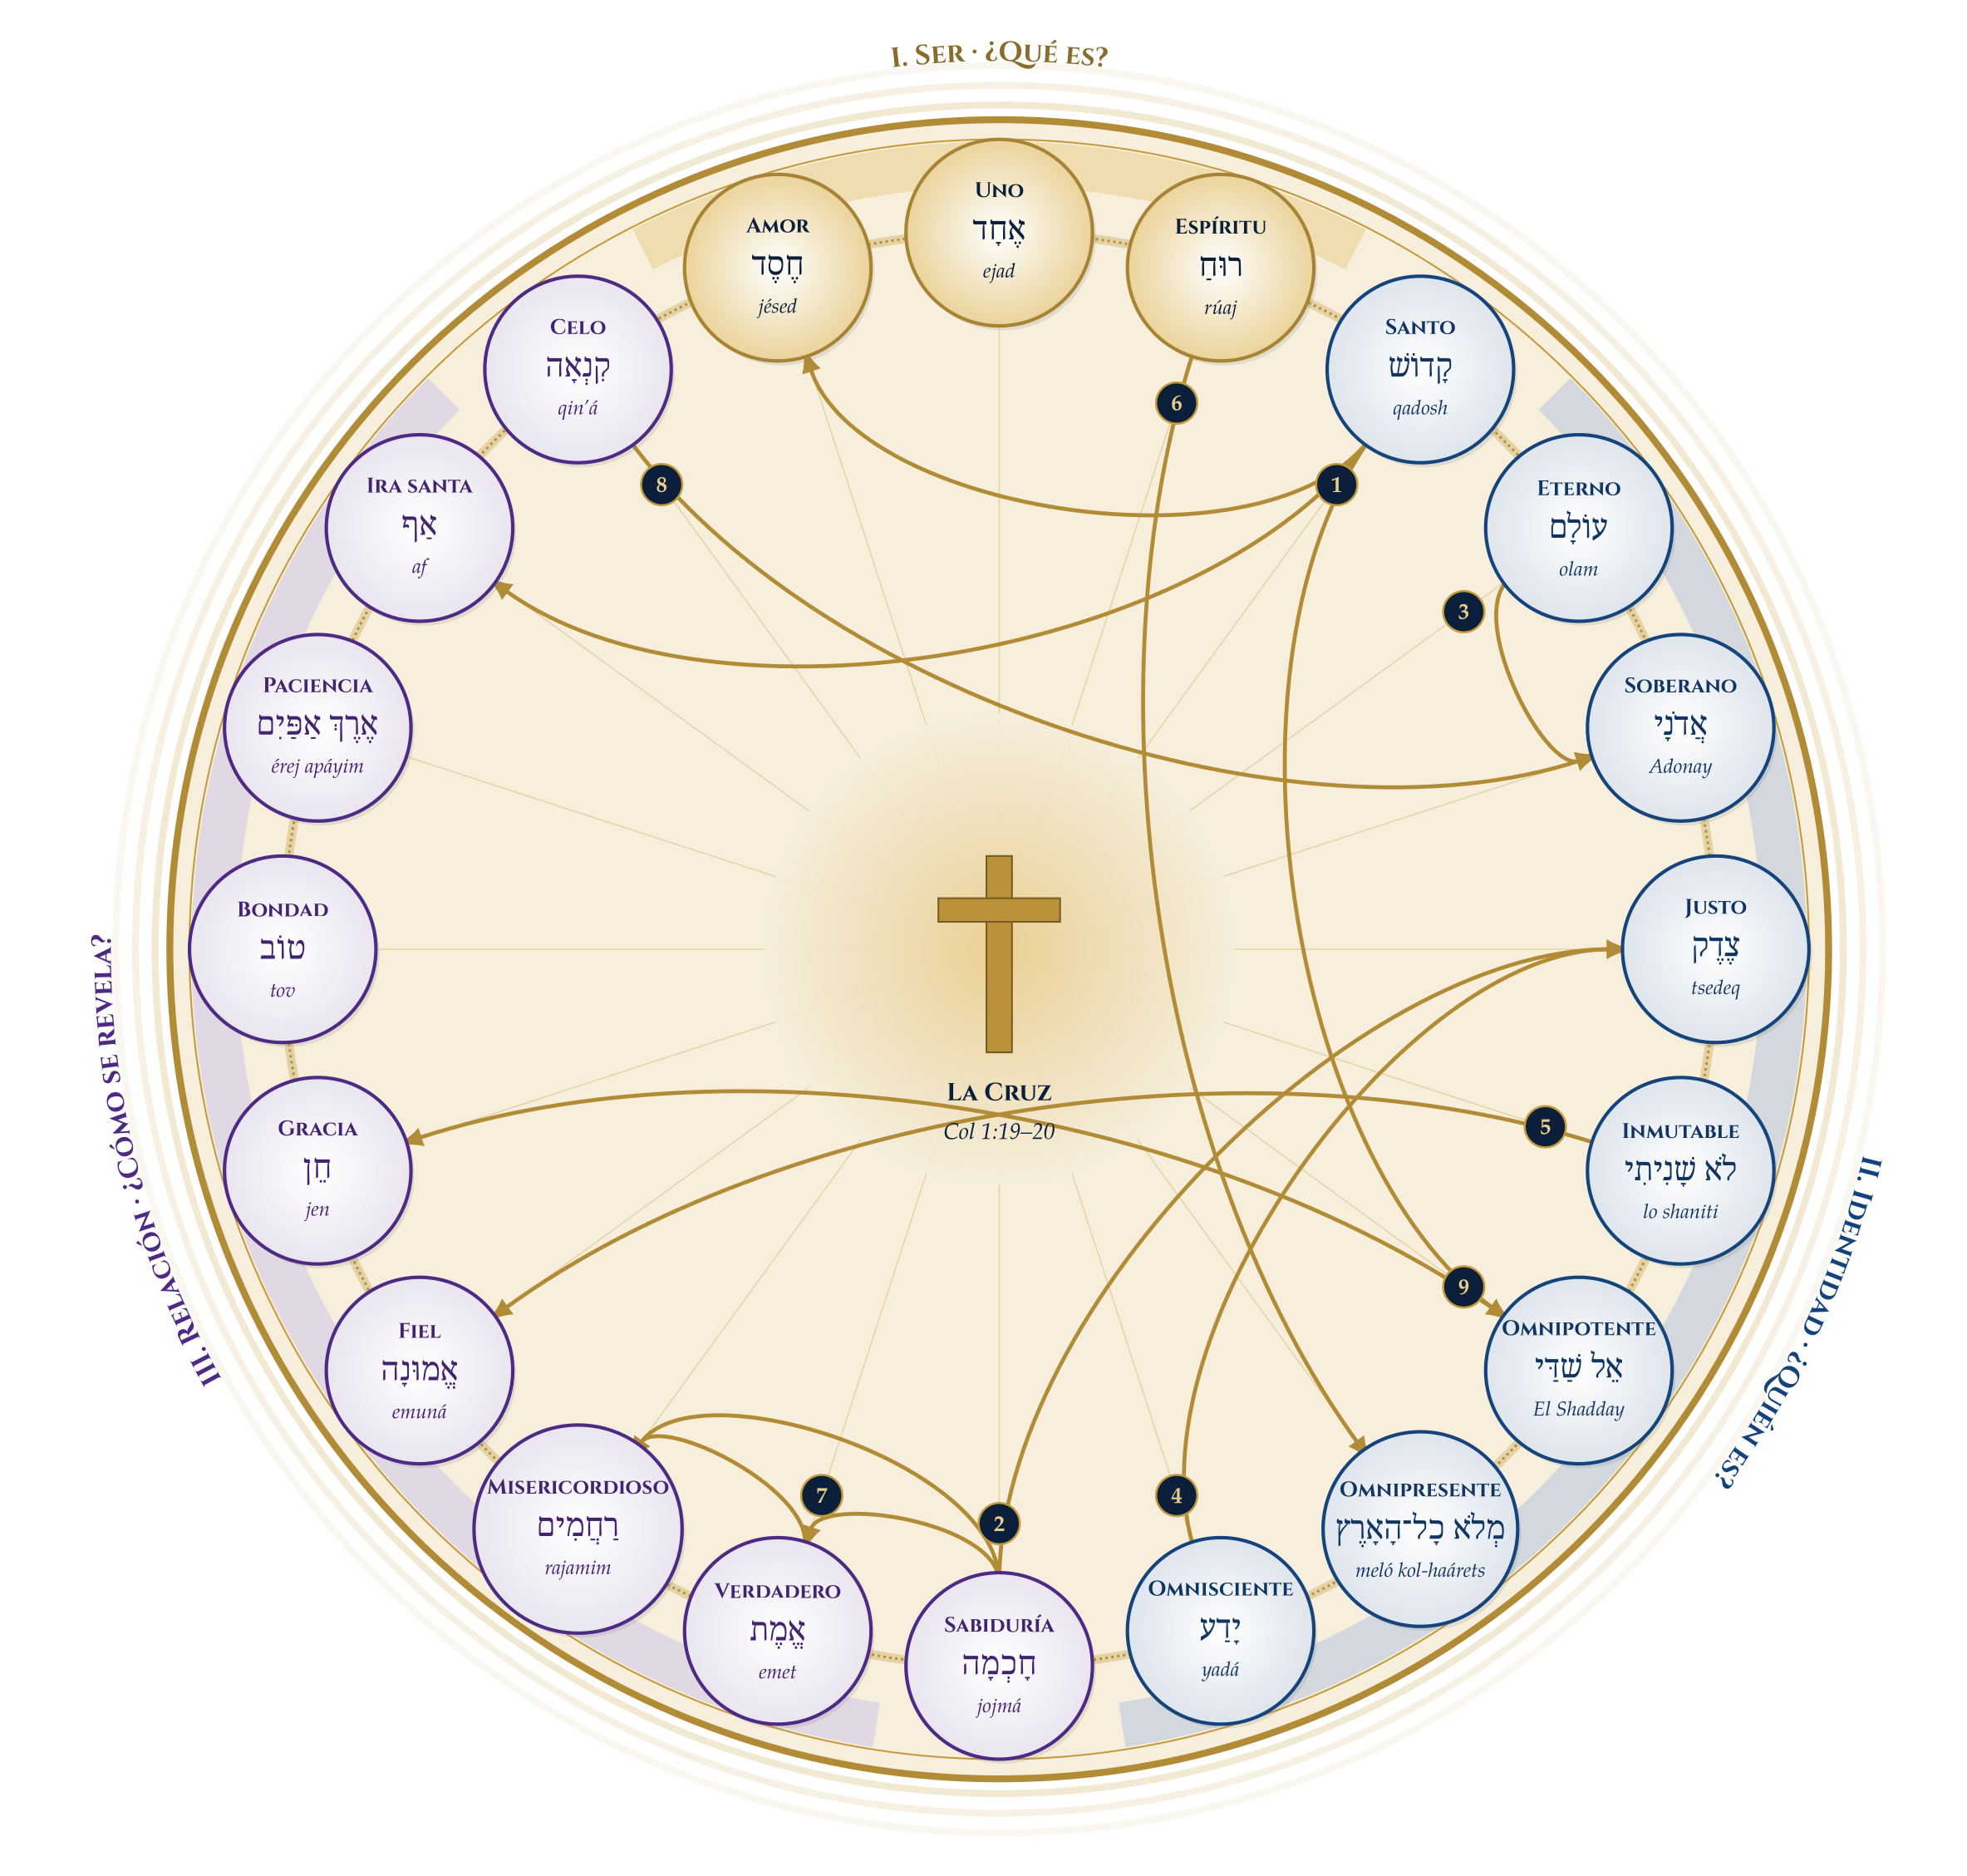
\includegraphics[width=0.80\linewidth]{img/sincronia_rosa_sinleyenda.png}};\end{tikzpicture}
\caption{Sincronía perfecta: cada atributo asegura a otro y todos convergen en la Cruz}\label{fig:sincronia-rosa}
\par{\footnotesize\color{gris}\textit{Nota.} Esquema del autor. Las flechas doradas van del atributo que asegura al atributo asegurado (números de la Tabla~\ref{tab:sincronia}); el anillo punteado es la unidad de Dios (Dt 6:4); los rayos indican la convergencia en Cristo (Col 1:19--20).}
\end{figure}

\begin{center}
\begin{tikzpicture}
\node[draw=azul,line width=0.8pt,rounded corners=3pt,inner sep=8pt,fill=white] (q)
  {\qrcode[height=2.6cm,level=M]{https://danilo-ds7.github.io/primera-linea/sincronia/}};
\node[anchor=west,text width=8.4cm,align=left,font=\small] at ([xshift=4mm]q.east)
  {\textbf{Diagrama interactivo.} Escanee el código para recorrer la sincronía: al tocar cada atributo se ve qué asegura, quién lo asegura y el texto bíblico que lo respalda.\\[3pt]
  {\footnotesize\color{gris}danilo-ds7.github.io/primera-linea/sincronia}};
\end{tikzpicture}
\end{center}

\subsection{Punto de convergencia: la Cruz}

Todo el cuadro desemboca en un solo acto. Pablo lo dice en el himno de Colosenses.

\par\smallskip{\centering\large\grc{ὅτι ἐν αὐτῷ εὐδόκησεν πᾶν τὸ πλήρωμα κατοικῆσαι καὶ δι᾽ αὐτοῦ ἀποκαταλλάξαι τὰ πάντα εἰς αὐτόν}\par}\smallskip

\begin{verso}{Colosenses 1:19–20}
por cuanto agradó al Padre que en él habitase toda plenitud, y por medio de él reconciliar consigo todas las cosas, así las que están en la tierra como las que están en los cielos, haciendo la paz mediante la sangre de su cruz.
\end{verso}

\begin{filologia}{Col 1:19--20}
\grc{πᾶν τὸ πλήρωμα} \emph{pan to plérōma} & \grc{πληρόω} & ``Toda la plenitud'': la totalidad de lo que Dios es; en 2:9, ``toda la plenitud de la Deidad''. \\
\grc{κατοικῆσαι} \emph{katoikēsai} & \grc{οἰκέω} & ``Habitar'' de modo permanente, establecerse; no una visita. \\
\grc{ἀποκαταλλάξαι} \emph{apokatalláxai} & \grc{ἀλλάσσω} & ``Reconciliar plenamente'': doble prefijo (\grc{ἀπο-}, \grc{κατα-}) sobre el verbo del canje de Ro 1:23. \\
\grc{εἰρηνοποιήσας} \emph{eirēnopoiésas} & \grc{εἰρήνη} & ``Haciendo la paz'': el \emph{shalom} de Sal 85:10 hecho en la sangre de la cruz. \\
\end{filologia}

En la Cruz los atributos que parecían opuestos actúan juntos. La ira fue satisfecha, porque Dios puso a Cristo ``como propiciación por medio de la fe en su sangre, para manifestar su justicia'' (Ro 3:25). La justicia fue honrada: Dios es ``el justo, y el que justifica al que es de la fe de Jesús'' (Ro 3:26). La misericordia fue derramada: ``siendo enemigos, fuimos reconciliados con Dios por la muerte de su Hijo'' (Ro 5:10). La santidad fue vindicada, porque el pecado no se ignoró, se juzgó. Y todo esto resultó en salvación para la humanidad y trajo la imagen visible del Dios invisible: ``El es la imagen del Dios invisible, el primogénito de toda creación'' (Col 1:15).

\precision{la correspondencia entre cada atributo y lo ocurrido en la Cruz es síntesis del autor sobre los textos citados.}

%===================================================================
\section{Síntesis}

Moisés pidió ver la gloria de Dios, y Dios le respondió haciendo pasar todo su bien y proclamando su Nombre: misericordioso, piadoso, tardo para la ira, grande en misericordia y verdad, justo (Éx 33:18--34:7). Eso es la gloria: el peso de todo lo que Dios es, la comunión de sus atributos. En la Torá se mostró en la nube, en el fuego del Sinaí y en la gloria que llenó el tabernáculo; en la historia de Israel se fue con el arca (Icabod) y con el templo (Ezequiel), y fue prometida de vuelta (Hag 2:9). Los Salmos la cantaron en la creación y en la Torá, la pidieron sobre toda la tierra y la dieron ``por tu misericordia, por tu verdad''. Los profetas la vieron santa, exclusiva y universal. En Jesús, el Verbo puso su tienda entre nosotros, ``lleno de gracia y de verdad'', y su gloria se vio en las señales, en el monte y, sobre todo, en la cruz. Pablo la reconoció en ``la faz de Jesucristo'', en quien ``habita corporalmente toda la plenitud de la Deidad''. Y los que lo contemplan son transformados ``de gloria en gloria'' hasta ser semejantes a Él.

\begin{tcolorbox}[enhanced,colback=papiro,colframe=azul,boxrule=1pt,arc=3pt,title={La gloria de Dios},fonttitle=\bfseries,colbacktitle=azul,coltitle=white]
La gloria de Dios es la comunión perfecta de todos sus atributos: el \emph{kavod}, el peso infinito de lo que Dios es (Éx 33:18--34:7). Se manifiesta en la creación (Sal 19:1; Ro 1:20), en la historia de Israel (Éx 40:34; Ez 43:2) y, en plenitud, en Jesucristo, en quien ``habita corporalmente toda la plenitud de la Deidad'' (Col 2:9) y en cuyo rostro brilla ``el conocimiento de la gloria de Dios'' (2 Co 4:6). No se comparte con los ídolos (Is 42:8), pero se comunica a los que están en Cristo, que son transformados ``de gloria en gloria'' (2 Co 3:18; Ro 8:30). Al ser humano le corresponde reconocerla: ``No a nosotros\ldots{} sino a tu nombre da gloria'' (Sal 115:1).
\end{tcolorbox}

\begin{figure}[htbp]
\centering
\begin{tikzpicture}\node[inner sep=0pt]{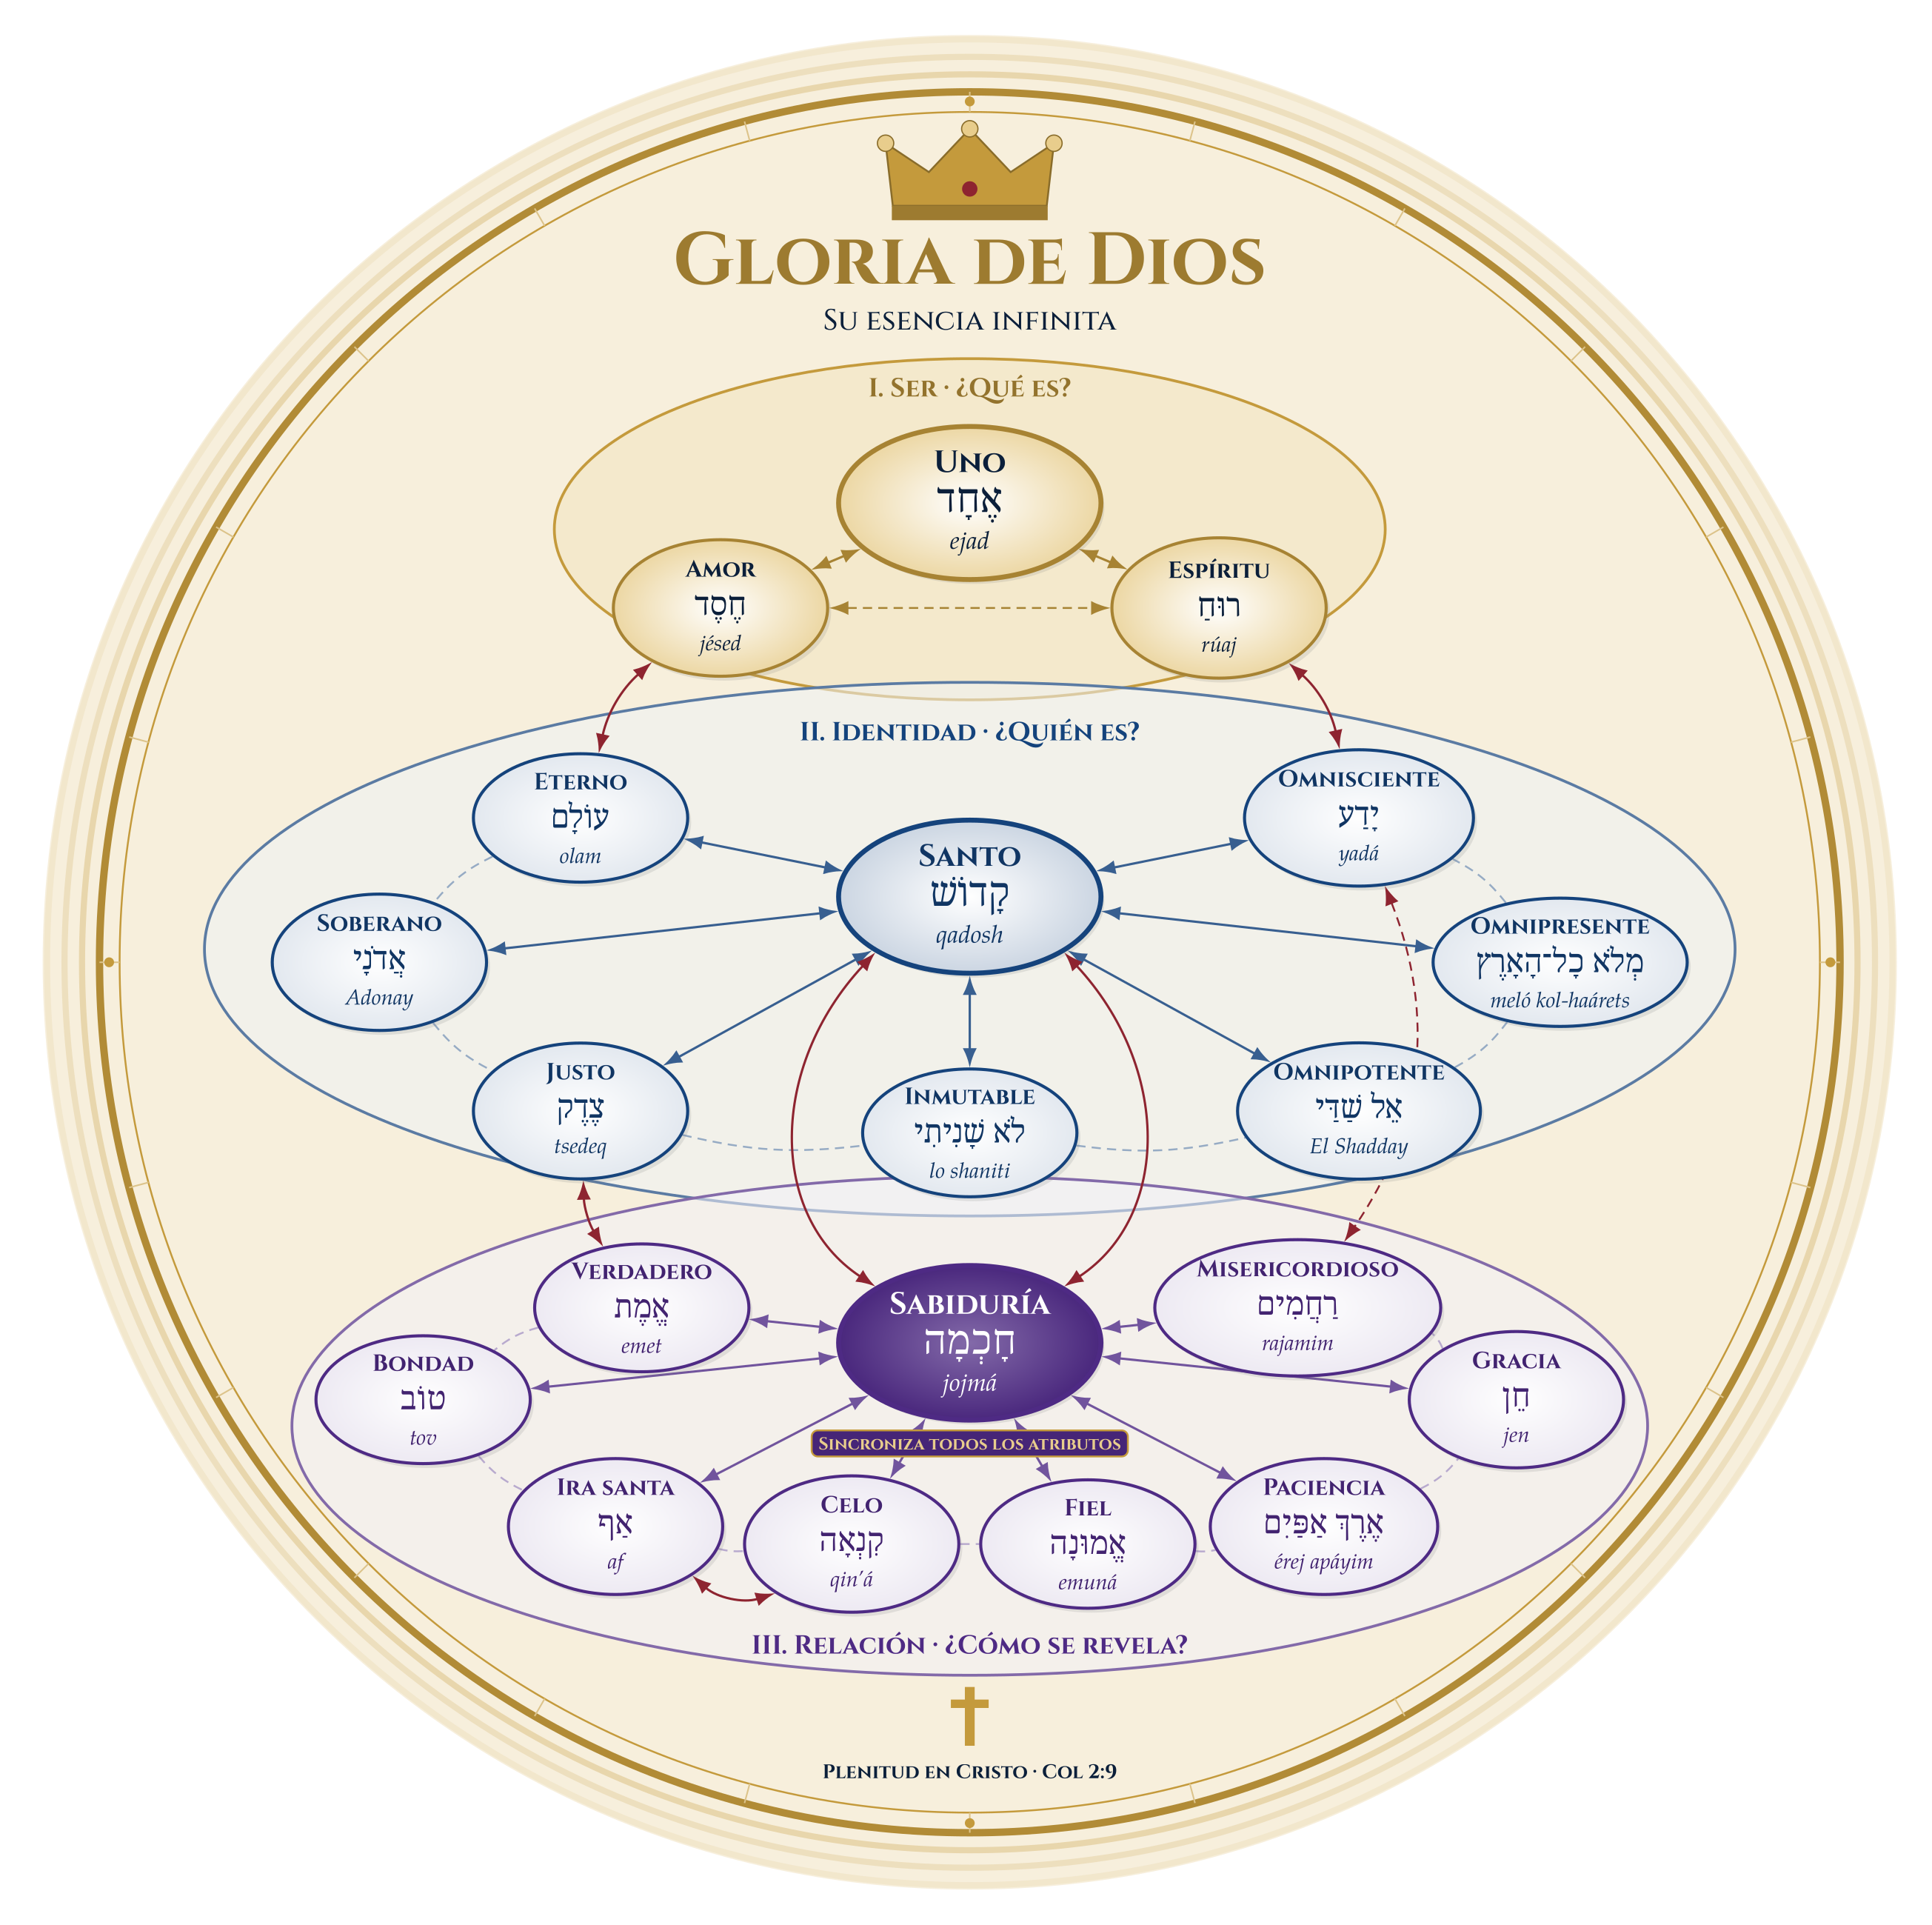
\includegraphics[width=0.80\linewidth]{img/gloria_esquema.png}};\end{tikzpicture}
\caption{Gloria de Dios: su esencia infinita}\label{fig:gloria-tikz}
\par{\footnotesize\color{gris}\textit{Nota.} Esquema del autor de la serie: los atributos del Ser, de la Identidad y de la Relación, sincronizados por la sabiduría. Uno es la base, Santo permea la identidad y todo converge en Cristo (Col 2:9).}
\end{figure}

\begin{center}\small\renewcommand{\arraystretch}{1.18}
\begin{tabular}{@{}L{2.4cm}L{11.4cm}@{}}
\toprule
\textbf{Mirada} & \textbf{Aporte a la gloria} \\ \midrule
Hebrea & \emph{kavod}, ``peso'': riqueza, honra, el yo, el resplandor; la gloria que reposa, llena y se va; Elí ``pesado'' e Icabod; el Nombre como gloria proclamada (Éx 34:6--7). \\
Judía & La Shejiná que acompaña al pueblo en el exilio (\emph{Meguilá} 29a); el segundo templo sin Shejiná (\emph{Yomá} 21b); todo creado para su gloria (\emph{Avot} 6:11); la \emph{Qedushá}; los atributos de acción (Maimónides). \\
Pink & La gloria esencial no aumenta ni disminuye; lo que crece es la manifiesta y su reconocimiento; ``el nombre es la colección de sus atributos''. \\
Paulina & La creación y la cruz (Ro 1; 3); ``gloríese en el Señor'' (Jer 9:24 en 1 Co 1:31); ``de gloria en gloria'' (2 Co 3:18); ``eterno peso de gloria''; toda la plenitud en Cristo (Col 1:19; 2:9). \\
\bottomrule
\end{tabular}\end{center}

El libro empezó con Jeremías 9:24 y termina con él. ``Mas alábese en esto el que se hubiere de alabar: en entenderme y conocerme, que yo soy \SENOR, que hago misericordia, juicio y justicia en la tierra''. Conocer a Dios en sus atributos no es un ejercicio académico: es la única gloria que no aplasta al que la lleva. Todo lo demás, sabiduría, fuerza, riqueza o fama, termina siendo demasiado liviano o demasiado pesado. La gloria de Dios, en cambio, es un peso que levanta: ``Mas tú, \SENOR, eres escudo alrededor de mí; mi gloria, y el que levanta mi cabeza'' (Sal 3:3).

En la Cruz no vemos a los atributos de Dios compitiendo entre sí, sino convergiendo en una sincronía perfecta. Allí la ira de Dios fue satisfecha, la justicia fue honrada, la misericordia fue derramada y la santidad fue vindicada. El celo del \SENOR{} revirtió el canje de Romanos 1 para devolvernos la imagen del Dios invisible, revelando que nuestro Dios es, hoy y siempre, soberana y perfectamente Uno (\heb{אֶחָד}, \emph{ejad}).

\begin{verso}{Romanos 11:36}
Porque de él, y por él, y para él, son todas las cosas. A él sea la gloria por los siglos. Amén.
\end{verso}

%===================================================================
\section*{Glosario del capítulo}
\begin{description}\setlength{\itemsep}{2pt}
\item[\emph{Allassō}] (\grc{ἀλλάσσω}). Cambiar, alterar; el verbo del canje de la gloria (Ro 1:23).
\item[\emph{Apokatallassō}] (\grc{ἀποκαταλλάσσω}). Reconciliar plenamente (Col 1:20); compuesto de la misma raíz.
\item[\emph{Aspaqlaria}] (\heb{אַסְפַּקְלַרְיָא}). ``Espejo, vidrio''; en el Talmud, la visión de los profetas (\emph{Yevamot} 49b).
\item[\emph{Doxa}] (\grc{δόξα}). ``Opinión, reputación'' en el griego clásico; ``gloria, resplandor'' en la Septuaginta y el Nuevo Testamento.
\item[\emph{Doxazō}] (\grc{δοξάζω}). Glorificar, honrar, hacer visible la gloria (Jn 12:28; Ro 8:30).
\item[\emph{Eskēnōsen}] (\grc{ἐσκήνωσεν}). ``Puso su tienda, habitó'' (Jn 1:14); de \grc{σκηνή}, tabernáculo.
\item[\emph{Hithalel}] (\heb{הִתְהַלֵּל}). Gloriarse, alabarse (Jer 9:23--24); en griego, \grc{καυχάομαι}.
\item[\emph{Icabod}] (\heb{אִי־כָבוֹד}). ``¿Dónde está la gloria?'' o ``sin gloria'' (1 S 4:21).
\item[\emph{Kaved}] (\heb{כָּבֵד}). Pesado; también ``honrar'' en la forma \emph{kibbed} (Éx 20:12).
\item[\emph{Kavod}] (\heb{כָּבוֹד}). Peso, riqueza, honra, gloria; la presencia manifiesta de Dios.
\item[\emph{Metallassō}] (\grc{μεταλλάσσω}). Intercambiar, dar una cosa por otra (Ro 1:25--26).
\item[\emph{Metamorphoō}] (\grc{μεταμορφόω}). Transformar, transfigurar (Mt 17:2; Ro 12:2; 2 Co 3:18).
\item[\emph{Mishkán}] (\heb{מִשְׁכָּן}). Morada, tabernáculo; de \heb{שָׁכַן}, habitar.
\item[\emph{Plērōma}] (\grc{πλήρωμα}). Plenitud (Col 1:19; 2:9).
\item[\emph{Qedushá}] (\heb{קְדֻשָּׁה}). Oración de la sinagoga que une Is 6:3 y Ez 3:12.
\item[\emph{Shejiná}] (\heb{שְׁכִינָה}). La presencia de Dios que habita; término posbíblico (targumes, Talmud).
\item[\emph{Theiotēs} / \emph{theotēs}] (\grc{θειότης} / \grc{θεότης}). Cualidad divina (Ro 1:20) / Deidad misma (Col 2:9).
\item[\emph{Tif'éret}] (\heb{תִּפְאֶרֶת}). Hermosura, ornamento, gloria (Éx 28:2).
\item[\emph{Yeqará}] (\heb{יְקָרָא}). ``Honra, lo precioso''; con ella traduce Ónkelos el \emph{kavod} de Dios.
\end{description}

